%%%%%%%%%%%%%%%%%%%%%%%%%%%%%%%%%%%%%%%%%%%%%%%%%%%%%%%%%%%%%%%%%%%%%%%%%%%%%%%%%%%%%%%%%%%%%%%%%%%%%%%
%%													%%
%% 	DIPLOMOVÁ PRÁCE -  Návrh webového administrátorského rozhraní pro platformu GIS.lab			%%
%% 				 David Zahradník							%%
%%													%%
%% pro formátování využita šablona: http://geo3.fsv.cvut.cz/kurzy/mod/resource/view.php?id=775 	%%
%%													%%
%%%%%%%%%%%%%%%%%%%%%%%%%%%%%%%%%%%%%%%%%%%%%%%%%%%%%%%%%%%%%%%%%%%%%%%%%%%%%%%%%%%%%%%%%%%%%%%%%%%%%%% 

\documentclass[%
  12pt,         			% Velikost základního písma je 12 bodů
  a4paper,      			% Formát papíru je A4
  oneside,       			% Oboustranný tisk
  pdftex,				    % překlad bude proveden programem 'pdftex' do PDF
%%%  draft
]{report}       			% Dokument třídy 'zpráva'
%

\newcommand{\Fbox}[1]{\fbox{\strut#1}}

\usepackage[czech, english]{babel}	% použití češtiny, angličtiny
\usepackage[utf8]{inputenc}		% Kódování zdrojových souborů je UTF8

\usepackage[square,sort,comma,numbers]{natbib}

\usepackage{caption}
\usepackage{subcaption}
\captionsetup{font=small}
\usepackage{enumitem} 
\setlist{leftmargin=*} % bez odsazení

\makeatletter
\setlength{\@fptop}{0pt}
\setlength{\@fpbot}{0pt plus 1fil}
\makeatletter

\usepackage[dvips]{graphicx}   
\usepackage{color}
\usepackage{transparent}
\usepackage{wrapfig}
\usepackage{float} 

\usepackage{cmap}           
\usepackage[T1]{fontenc}    

\usepackage{textcomp}
\usepackage[compact]{titlesec}
\usepackage{amsmath}
\addtolength{\jot}{1em} 

\usepackage{chngcntr}
\counterwithout{footnote}{chapter}

\usepackage{acronym}

\usepackage[
    unicode,                
    breaklinks=true,        
    hypertexnames=false,
    colorlinks=true, % true for print version
    citecolor=black,
    filecolor=black,
    linkcolor=black,
    urlcolor=black
]{hyperref}         

\usepackage{url}
\usepackage{fancyhdr}
%\usepackage{algorithmic}
\usepackage{algorithm}
\usepackage{algcompatible}
\renewcommand{\ALG@name}{Pseudokód}% Update algorithm name
\def\ALG@name{Pseudokód}

\usepackage[
  cvutstyle,          
  diploma           
]{thesiscvut}


\newif\ifweb
\ifx\ifHtml\undefined % Mimo HTML.
    \webfalse
\else % V HTML.
    \webtrue
\fi 

\renewcommand{\figurename}{Obrázek}
\def\figurename{Obrázek}

%%%%%%%%%%%%%%%%%%%%%%%%%%%%%%%%%%%%%%%%%%%%%%%%%%%%%%%%%%%%%%%%%
%%%%%%%%%%% Definice informací o dokumentu  %%%%%%%%%%%%%%%%%%%%%
%%%%%%%%%%%%%%%%%%%%%%%%%%%%%%%%%%%%%%%%%%%%%%%%%%%%%%%%%%%%%%%%%

%% Název práce
\nazev{Konstrukce bezpilotního letadla pro geodetické práce}
{sdgfdg}


%% Jméno a příjmení autora
\autor{Bc. David}{Zahradník}

%% Jméno a příjmení vedoucího práce včetně titulů
\garant{Ing.~Zdeněk~Vyskočil,~Ph.D.}

%% Označení programu studia
\programstudia{Geodézie a~kartografie}{}

%% Označení oboru studia
\oborstudia{Geomatika}{}

%% Označení ústavu
\ustav{Katedra geomatiky}{}

%% Rok obhajoby
\rok{2019}

%Mesic obhajoby
\mesic{červen}

%% Místo obhajoby
\misto{Praha}

%% Abstrakt
\abstrakt {Tato diplomová práce se konstrukcí bezpilotního letadla pro geodetické účely na platformě Arduino s Arduino periferiemi}  {This thesis describes construction of unmanned uerial vehicle for surveying jobs using Arduino platform and Arduino moduls.}

%% Klíčová slova
\klicovaslova
{bezpilotní letadlo, dron, Arduino, Android,}
{UAV, dron, Arduino, Android}

%%%%%%%%%%%%%%%%%%%%%%%%%%%%%%%%%%%%%%%%%%%%%%%%%%%%%%%%%%%%%%%%%%%%%%%%

%%%%%%%%%%%%%%%%%%%%%%%%%%%%%%%%%%%%%%%%%%%%%%%%%%%%%%%%%%%%%%%%%%%%%%%%
%% Nastavení polí ve Vlastnostech dokumentu PDF
%%%%%%%%%%%%%%%%%%%%%%%%%%%%%%%%%%%%%%%%%%%%%%%%%%%%%%%%%%%%%%%%%%%%%%%%
\nastavenipdf
%%%%%%%%%%%%%%%%%%%%%%%%%%%%%%%%%%%%%%%%%%%%%%%%%%%%%%%%%%%%%%%%%%%%%%%

%%% Začátek dokumentu
\begin{document}

\catcode`\-=12  % pro vypnuti aktivniho znaku '-' pouzivaneho napr. v \cline 

% aktivace záhlaví
\zahlavi

% předefinování vzhledu záhlaví
\renewcommand{\chaptermark}[1]{%
	\markboth{\MakeUppercase
	{%
	\thechapter.%
	\ #1}}{}}

% Vysázení přebalu práce
%\vytvorobalku

% Vysázení titulní stránky práce
\vytvortitulku {}

% Vysázení listu zadani
\stranka{}%
	{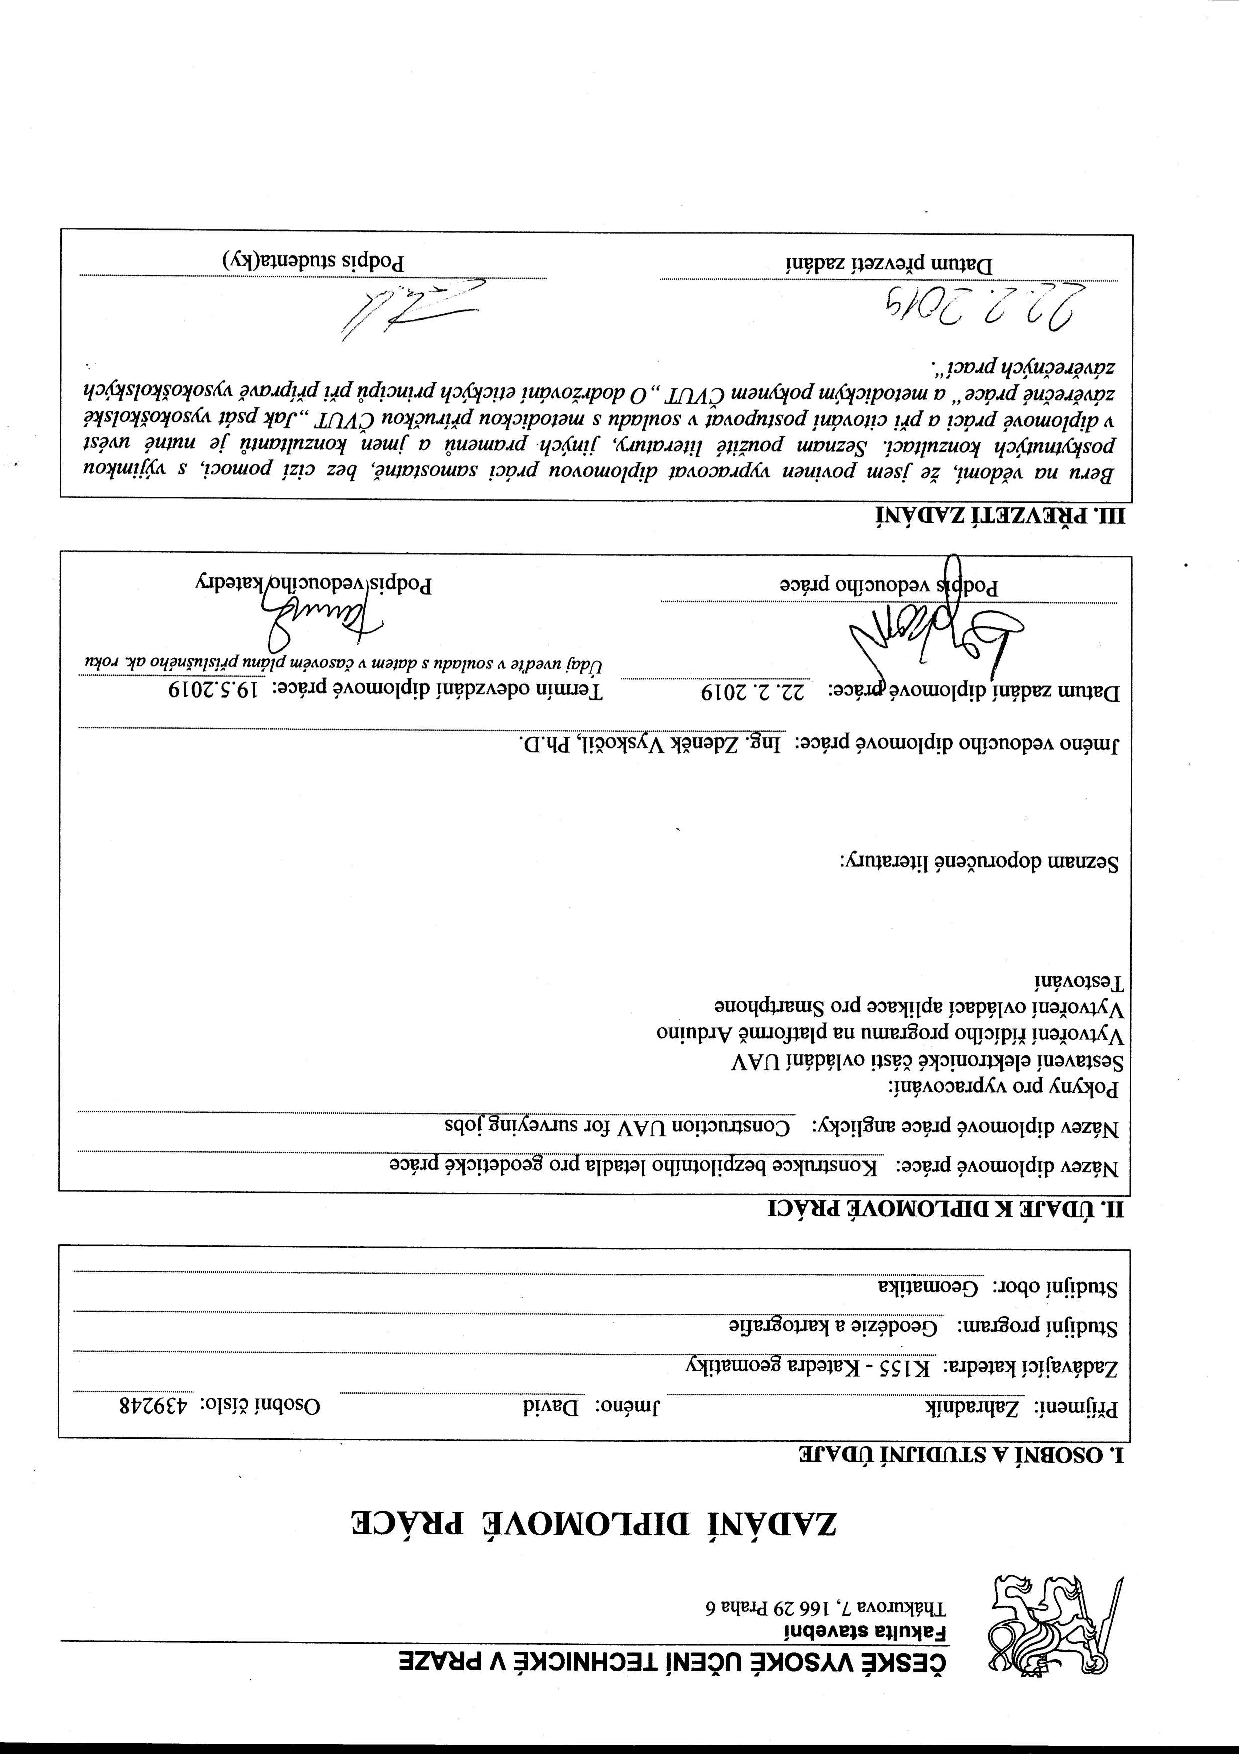
\includegraphics[scale=0.7,angle=180]{./pictures/zadani.pdf}
	}%\sffamily\Huge\centering\ }%ZDE VLOŽIT LIST ZADÁNÍ}%
	%{\sffamily\centering Z~důvodu správného číslování stránek}

% Vysázení stránky s abstraktem
\vytvorabstrakt

% Vysázení prohlaseni o samostatnosti
\vytvorprohlaseni

% Vysázení poděkování
\stranka{%nahore
       }{%uprostred
       }{%dole
       \sffamily
	\begin{flushleft}
		\large
		\MakeUppercase{Poděkování}
	\end{flushleft}
	\vspace{1em}
		%\noindent
	\par\hspace{2ex}
	{Chtěl bych poděkovat Ing. Zdeňku Vyskočilovi Ph.D. za pomoc a rady při zpracování diplomové práce. Dále bych rád poděkoval Lukáši Černému za poskytnuté rady a vysvětlení témat týkajících se elektrotechniky.}
}

% Vysázení obsahu
\obsah

% Vysázení seznamu obrázků
\seznamobrazku

% Vysázení seznamu tabulek
\seznamtabulek

% jednotlivé kapitoly
\chapter{Úvod}
\label{0-uvod}


Bezpilotní letadla neboli drony jsou rychle vyvíjeným odvětvím v zeměměřičství. Nedostatek kvalitní pracovní síly nahrává automatizaci sběru dat, tedy dronům a skenerům.\\
V dnešní době dron plní funkci nosiče fotogrammetrické kamery nebo skeneru. Využívá se pro sběr objemných dat za velmi krátkou dobu. Výsledky po zpracování jsou ortofota, fotoplány, mračna bodů a z nich 3D modely.\\
V této diplomové práci je popisována stavba dronu na platformě Aurduino, který by mohl nahradit výtyčku při různých zeměměřičských pracích.\\
Pokud by se na dron implementovala GNSS aparatura s podporou metody RTK, dal by se dron využít pro vytyčování. Po zadání souřadnic uživatelem, by dron přeletěl na zadané místo a přistál by. Po příchodu uživatele by dron vzletěl, držel by pozici zadaných souřadnic a uživatel by stabilizoval bod podle laserové stopy.\\
Další možností by bylo připevnění laserového dálkoměru na dron a implementaci automatického cílení dle hranolu drženého uživatelem na zemi, dron by držel pozici nad hranolem. Využití by se našlo v nepříznivých oblastech pro GNSS aparatury (vysoké objekty: stromy, budovy). Dron s GNSS aparaturou by létal nad vysokými objekty s ideální konfigurací satelitů a uživatel by s hranolem na zemi měřil polohu přes GNSS na dronu.\\
Pokud by dron dokázal komunikovat s totální stanicí, získali bychom přesné souřadnice letu dronu, které by se daly použít pro přesné definování letové dráhy. Využití by se našlo při měření skal, mostů a sloupů.\\
Pro uskutečnění nápadů je potřeba znát problematiku letu dronu, proto se diplomová práce zabývá konstrukcí dronu. V práci se čtenář dozví o teorii letu dronů, použitých komponent pro stavbu a následném sestavování.\\

%V úvodu práce se čtenář dozví něco málo o teorii létání dronů. V následující kapitole jsou uvedeny komponenty a jejich popis. V kapitole Konstrukce jsou prvně vysvětleny dílčí kroky a následně celkový přehled o propojení komponent a popis algoritmu, který ovládá dron. Pro ovládání byla vytvořena aplikace pro mobilní operační systém Android, její uživatelský manuál je popsán v Ovládání.\\
\chapter{Rešerše}
\label{1-reserse}

Bezpilotní letadla/drony jsou fenoménem dnešního stolení, zabývá se jimi spousta článku a projektů. \\
Projekt YMFC-32\\
%http://www.brokking.net/

Projekt popisuje stavbu drona/quadrocoptéry ovládaného přes RC soupravu. Pro ovládání motorů na dronu byla použita platforma Arduino a periferie Arduina (IMU, Bluetooth).\\

Univerzální software pro ovládání RC modelu\\
%http://www.multiwii.com/
Software je používán pro stavbu drona na platformě Arduino. Software má předdefinované různé typy dronů a Arduino periferíí.\\

Projekt Arduino quadrocopter\\
%http://mydronelab.com/blog/arduino-quadcopter.html
Projekt se zabývá stavbou quadrokopéry na platformě Arduino s využitím softwaru  Multiwii.\\

%https://www.geobusiness.cz/soutez-dronapp-2018/
\chapter{Teorie}
\label{2-teorie}

Nejdůležitějšími prvky dronu jsou motory s vrtulemi, mikroprocesor a IMU. Motory s vrtulemi fungují jako ventilátory, které ženou vzduch určitým směrem, pokud všechny motory ženou vzduch proti zemi, dron by měl vzlétnout. Proč je tedy potřeba mikroprocesor a IMU? Bohužel rozložení hmotnosti dronu a drobné mechanické rozdíly v motorech, zapříčiní různé tahy jednotlivých motorů. Díky ovládání motorů podle mikroprocesoru, dokážeme vliv různých tahů vyrovnat a dron může létat.\\
Jakým způsobem vykonává dron pohyb? Let dronu v určitém směru je způsoben snížením výkonu motorů ve směru letu a zvýšením výkonu motorů v opačném směru letu, viz obrázek č. 3.1. Rotace dronu je uskutečněna zvýšením výkonu motorů s různými typy vrtulí, směrem hodinových ručiček a proti (CW a CCW orientace). Zvýšením výkonu na motorech s vrtulemi s orientací CW se dron otáčí po směru hodinových ručiček, s orientací CCW proti směru hodinových ručiček, viz obrázek 3.2.\\
%https://www.wired.com/2017/05/the-physics-of-drones/

\begin{figure}[H]
	\centering
	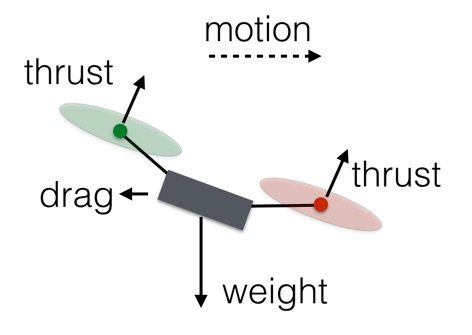
\includegraphics[width=7cm]{pictures/dronfly.jpg}
	\caption{Let určitým směrem(motion-směr, thrust/drag-tah, weigth-váha)}
	\cite{physicdrone}
\end{figure}
%https://devusa.djicdn.com/images/flightController-concepts/altitude-7e757661b6.png

\begin{figure}[H]
	\centering
	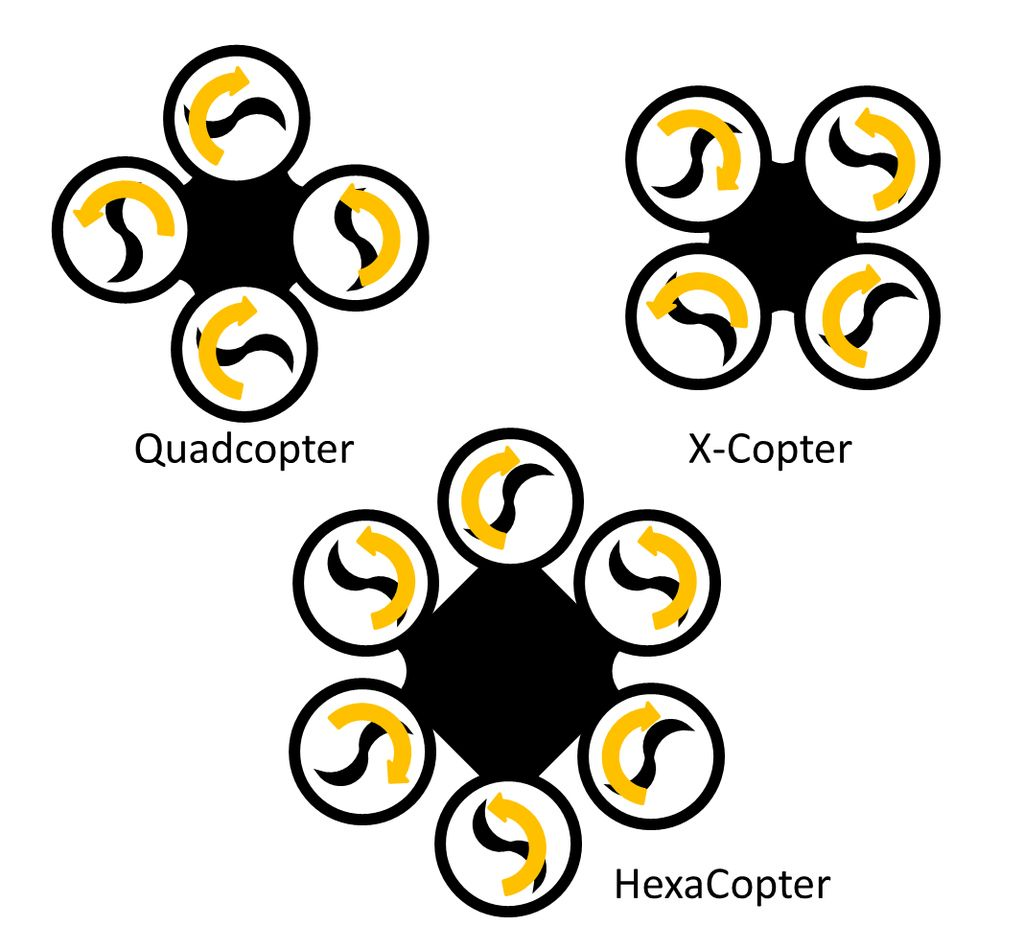
\includegraphics[width=10cm]{pictures/dronrot.png}
	\caption{Přehled vtrulí se CW a CCW orientací}
	\cite{rotdrone}
\end{figure} 
Důležitou roli při letu dronu hraje IMU jednotka, která určuje úhly rotace. Roll je úhel rotace kolem osy X, pitch je úhel rotace kolem osy Y a yaw je úhel rotace kolem osy Z. Souřadný systém má střed v težišti dronu. Osa X směřuje do směru letu, osa Y je na ni kolmá a osa Z je totožná s tížnicí, viz obrázek 3.3.\\
Řízení dronu probíhá přes jmenované úhly pitch, roll a yaw. Uživatel zadává úhly a mikrokprocesor podle IMU zadané úhly nastavuje. Nastavení úhlu vzniká pomocí zvyšování a snižování výkonu na jednotlivých motorech. Popis řízení dronu je podrobněji vysvětlen v kapitole Ovládání jednotlivých elektronických částí u Letového kontroléru.\\
Existuje vícero překladů úhlů pitch, roll a yaw (např. vybočení, klonění a  klopení, nebo příčný náklon, podélný sklon a zatáčení), pro zjednodušení bude v textu ponecháno pojmenování v anglickém jazyce.\\
%Source: https://www.instructables.com/id/Design-Build-and-Improve-a-Quadcopter/

\begin{figure}[H]
	\centering
	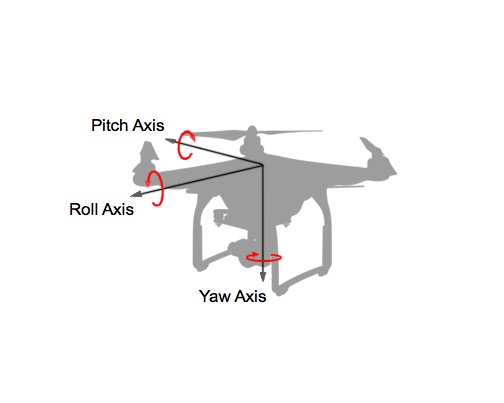
\includegraphics[width=10cm]{pictures/rotangle.png}
	\caption{Úhly rotace (Axis - Osa)}
	\cite{diffdrone}
\end{figure} 

\chapter{Komponenty}
\label{3-soucastky}

Při stavbě dronu je potřeba rozmyslet jeho účel, nosnost a délku letu. Od těchto myšlenek (potřeb) se odvíjí dílčí součástky a jejich parametry. Základními součástky jsou kostra, baterie, vrtule, motory, regulátory otáček, IMU, komunikační zařízení a řídící jednotka.\\
Důležitým faktorem je počet vrtulí/motorů. Podle počtu vrtulí dělíme drony na trikoptéry (3), quadrokopéry (4), hexakoptéry (6), a octokoptéry (8). Obecně platí, čím více má dron vrtulí, tím více je stabilnější, dokáže létat i při selhání z jednoho motorů (hexakoptéra a octokoptéra). Zároveň stavba dronu s vyšší počtem vrtulí je dražší a náročnější.\\
V této diplomové práci je popisována stavba hexakoptéry, jejíž kostra a motory byly použity z nefunkčního dronu of firmy Microkopter zapůjčeného z laboratoře fotogrammetrie.\\

\section{Kostra} 
Kostra by měla být lehká a pevná, nejčastěji se používá karbon a hliník pro stavbu dronu s vyšší nosností a plast pro ostatní drony. Kostra se skládá z centra, ramen, stojánku a držáků pro motory.\\
Jak už bylo zmíněno, byla použita kostra od firmy Microkopter. Stojánek je vyroben z karbonu, centrum z plastu, ramena a držáky motorů z hliníku.\\


\section{Baterie} 
Výběrovým kritériem pro baterie jsou kapacita, výstupní napětí, maximální vybíjecí proud.
Nejpoužívanějšími bateriemi pro stavbu dronu jsou LiPo baterie, které nejsou těžké, nemají paměťový efekt, při správném zacházení mají dlouhou životnost a vysoký vybíjecí proud.\\
Výstupní napětí ovlivňuje množství článků baterie. Jeden článek má hodnotu nominálního napětí 3.7V, při plném nabití článku 4.2V. Maximální vybíjecí proud je dán konstantou C. Je-li konstanta C rovna 25 a kapacita baterie je 6750 mA, lze bezpečně odebírat proud o velikosti cca 168 Ampérů. Maximální odběr nesmí být větší, může dojít k poškození baterie.\\
\begin{eqnarray*} 
	6.75A * 25C & = & 168.75A\\
\end{eqnarray*} 

\textbf{Parametry použité baterie}\\
%https://www.peckamodel.cz/ta-25c-6750-4s1p-gens-ace-lipo-tattu-serie-4s-6750-mah-25c\\
Počet článků: 4 (4S)\\
Napětí: 14.8V\\
Kapacita baterie: 6750mA\\
Maximální proudové zatížení: 25C (168.75A)\\
Maximální vybíjecí proud: 50C (337.5A)\\
Hmotnost: 605 g\\
Cena: 2500 Kč\\
\cite{baterie}\\

\textbf{Rady pro zacházení s LiPo bateriemi}\\
Nabíjet baterie proudem s 1C, tedy baterii s kapacitou 6750mA dobíjet proudem o velikkosti 6.75A.\\
Nepřebíjet baterie nad hodnotu napětí 4.2V na článek.\\
Nepodbíjet baterie pod napětí 2.7V.\\
Při delším skladování vybít na hodnotu napětí 3.3V na článek.\\
Pro podrobnější instrukce je potřeba si přečíst příbalový leták.\\

\section{Distribuční deska} 
Distribuční deska PCB neboli napájecí deska slouží k zapojení všech  komponent na baterii. Jednotlivá napájená místa jsou zapojena paralelně, aby při zkratu jednoho ze zařízení, ostatní zařízení fungovala. K desce lze připojit i zařízení s jiným vstupním napětím než je napětí baterie (5V, 12V).\\

\textbf{Parametry distribuční desky}\\
Matek PDB-XT60\\
Množství LiPo článků: 3S-4S\\
Vstup VCC, GND\\
Výstup, 6x + a -, 12V, 5V, 2x -\\
Cena: 130 Kč\\
\cite{pdb}\\
%https://www.rotorama.cz/prislusenstvi/matek-pdb-s-5v-12v

\begin{figure}[H]
	\centering
	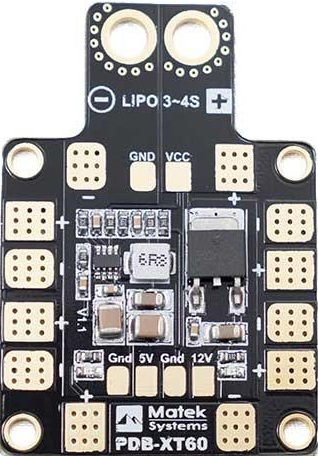
\includegraphics[width=3cm]{pictures/pdb.jpg}
	\caption{Distribuční deska - Matek PDB-XT60}
\end{figure}

\section{Vrtule} 
Vrtule generují tah dronu. Při stavbě dronu jsou potřeba dva typy vrtulí, se směrem hodinových ručiček a proti. Dva typy vrtulí jsou potřeba pro rotaci dronu kolem svislé osy. Další parametry jsou průměr a rozteč, nejčastěji uvedená v palcích. Materiál použivaný na výrobu vrtulí je plast nebo karbon. Doporučuji při stavbě dronu a jeho testování používat plastové vrtule, jsou cenově méně náročné.\\

\textbf{Parametry použitých vrtulí}\\
Materiál: plast\\
Průměr: 12 palců\\
Rozteč: 3.8 palce\\
Cena: 6 x 100 Kč\\

\section{Bezkartáčové motory} 
%https://www.youtube.com/watch?v=bCEiOnuODac
%learnengineering
%https://www.mikrocontroller.com/index.php?main_page=product_info&cPath=73&products_id=887&zenid=e5f2c8d548f2a39747a4ed06d306a37f
%motor
BLDC motory mají výhodu především v dlouhé životnosti a v plynulém kroku. Motor se skládá z rotoru a statoru. Rotor je permanentní magnet, stator je prstenec uspořádaných cívek. Postupným pouštění proudu do cívek (vytvářením magnetického pole) se rotor začne pohybovat.\\
Cívky jsou rozdělené do skupiny A, B, C, což jsou i vstupní piny motorů.  Nedílnou součástí motorů je regulátor otáček ESC, který řídí vstupní proud přes piny A, B a C a tím ovlivňuje rychlost motoru. Prohozením pinů A a C určíme směr otáčení motoru, možnost otáčení lze změnit i při kalibraci regulátoru otáček.\cite{learnengineering}\\
Výběr motorů je závislý na konstatně Kv, parametrech baterie a parametrech regulátoru otáček. Hodnota Kv neboli rpm/V je konstanta, která popisuje rychlost otáčení motoru v závislosti na napětí baterie. Platí úměra, čím menší je hodnota Kv, tím větší je tah motoru  a menší rychlost otáčení. Naopak čím  větší je hodnota Kv, tím je menší tah a větší rychlost otáčení. V závodní dronech se používají motory s větší hodnotou Kv, pro fotogrammetrii motory s menší hodnotou Kv.\cite{kv} \cite{siieefpv}\\

%http://learningrc.com/motor-kv/
%kn
%https://www.youtube.com/watch?v=y199oKTlwxU
%siieefpv
\textbf{Parametry použitých motorů}\\
Firma: Microkopter\\
Množství LiPo článků: 4S-6S\\
Provozní napětí: 25A\\
Maximální provozní napětí 30A\\
Rychlost bez zatížení: 500 rpm/V\\
Nosnost: 2200g\\
Váha: 121g\\
Cena: 6x 1500 Kč\\
\cite{motor}\\

\section{Regulátory otáček} 
Regulátory otáček (ESC) jsou nedílnou součástí BLDC motorů. Regulátor je řídící jednotka motoru, která zajistí plynulý chod. Regulátor se ovládá přes různé komunikační protokoly, které jsou popsány v kapitole Konstrukce.\\

\textbf{Parametry použitých regulátorů otáček}\\
HGLRC BS30A\\
Vnitřní software: BLHeliSuite\\
Vstup: VCC (7.4V - 18.5V) ,GND, -, S\\
Výstup: A, B, C\\
Maximální proud: 30A / 40A max\\
Množství LiPo článků: 2S-5S\\
Použitá knihovna: Servo\\
Cena: 200 Kč\\
\cite{esc}\\
%https://www.rotorama.cz/regulatory/hglrc-bs30a

\begin{figure}[H]
	\centering
	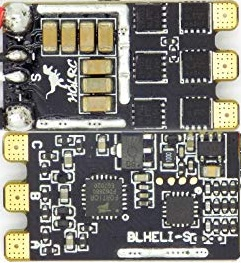
\includegraphics[width=4cm]{pictures/esc.jpg}
	\caption{Regulátor otáček - HGLRC BS30A}
\end{figure}

\begin{figure}[H]
	\centering
	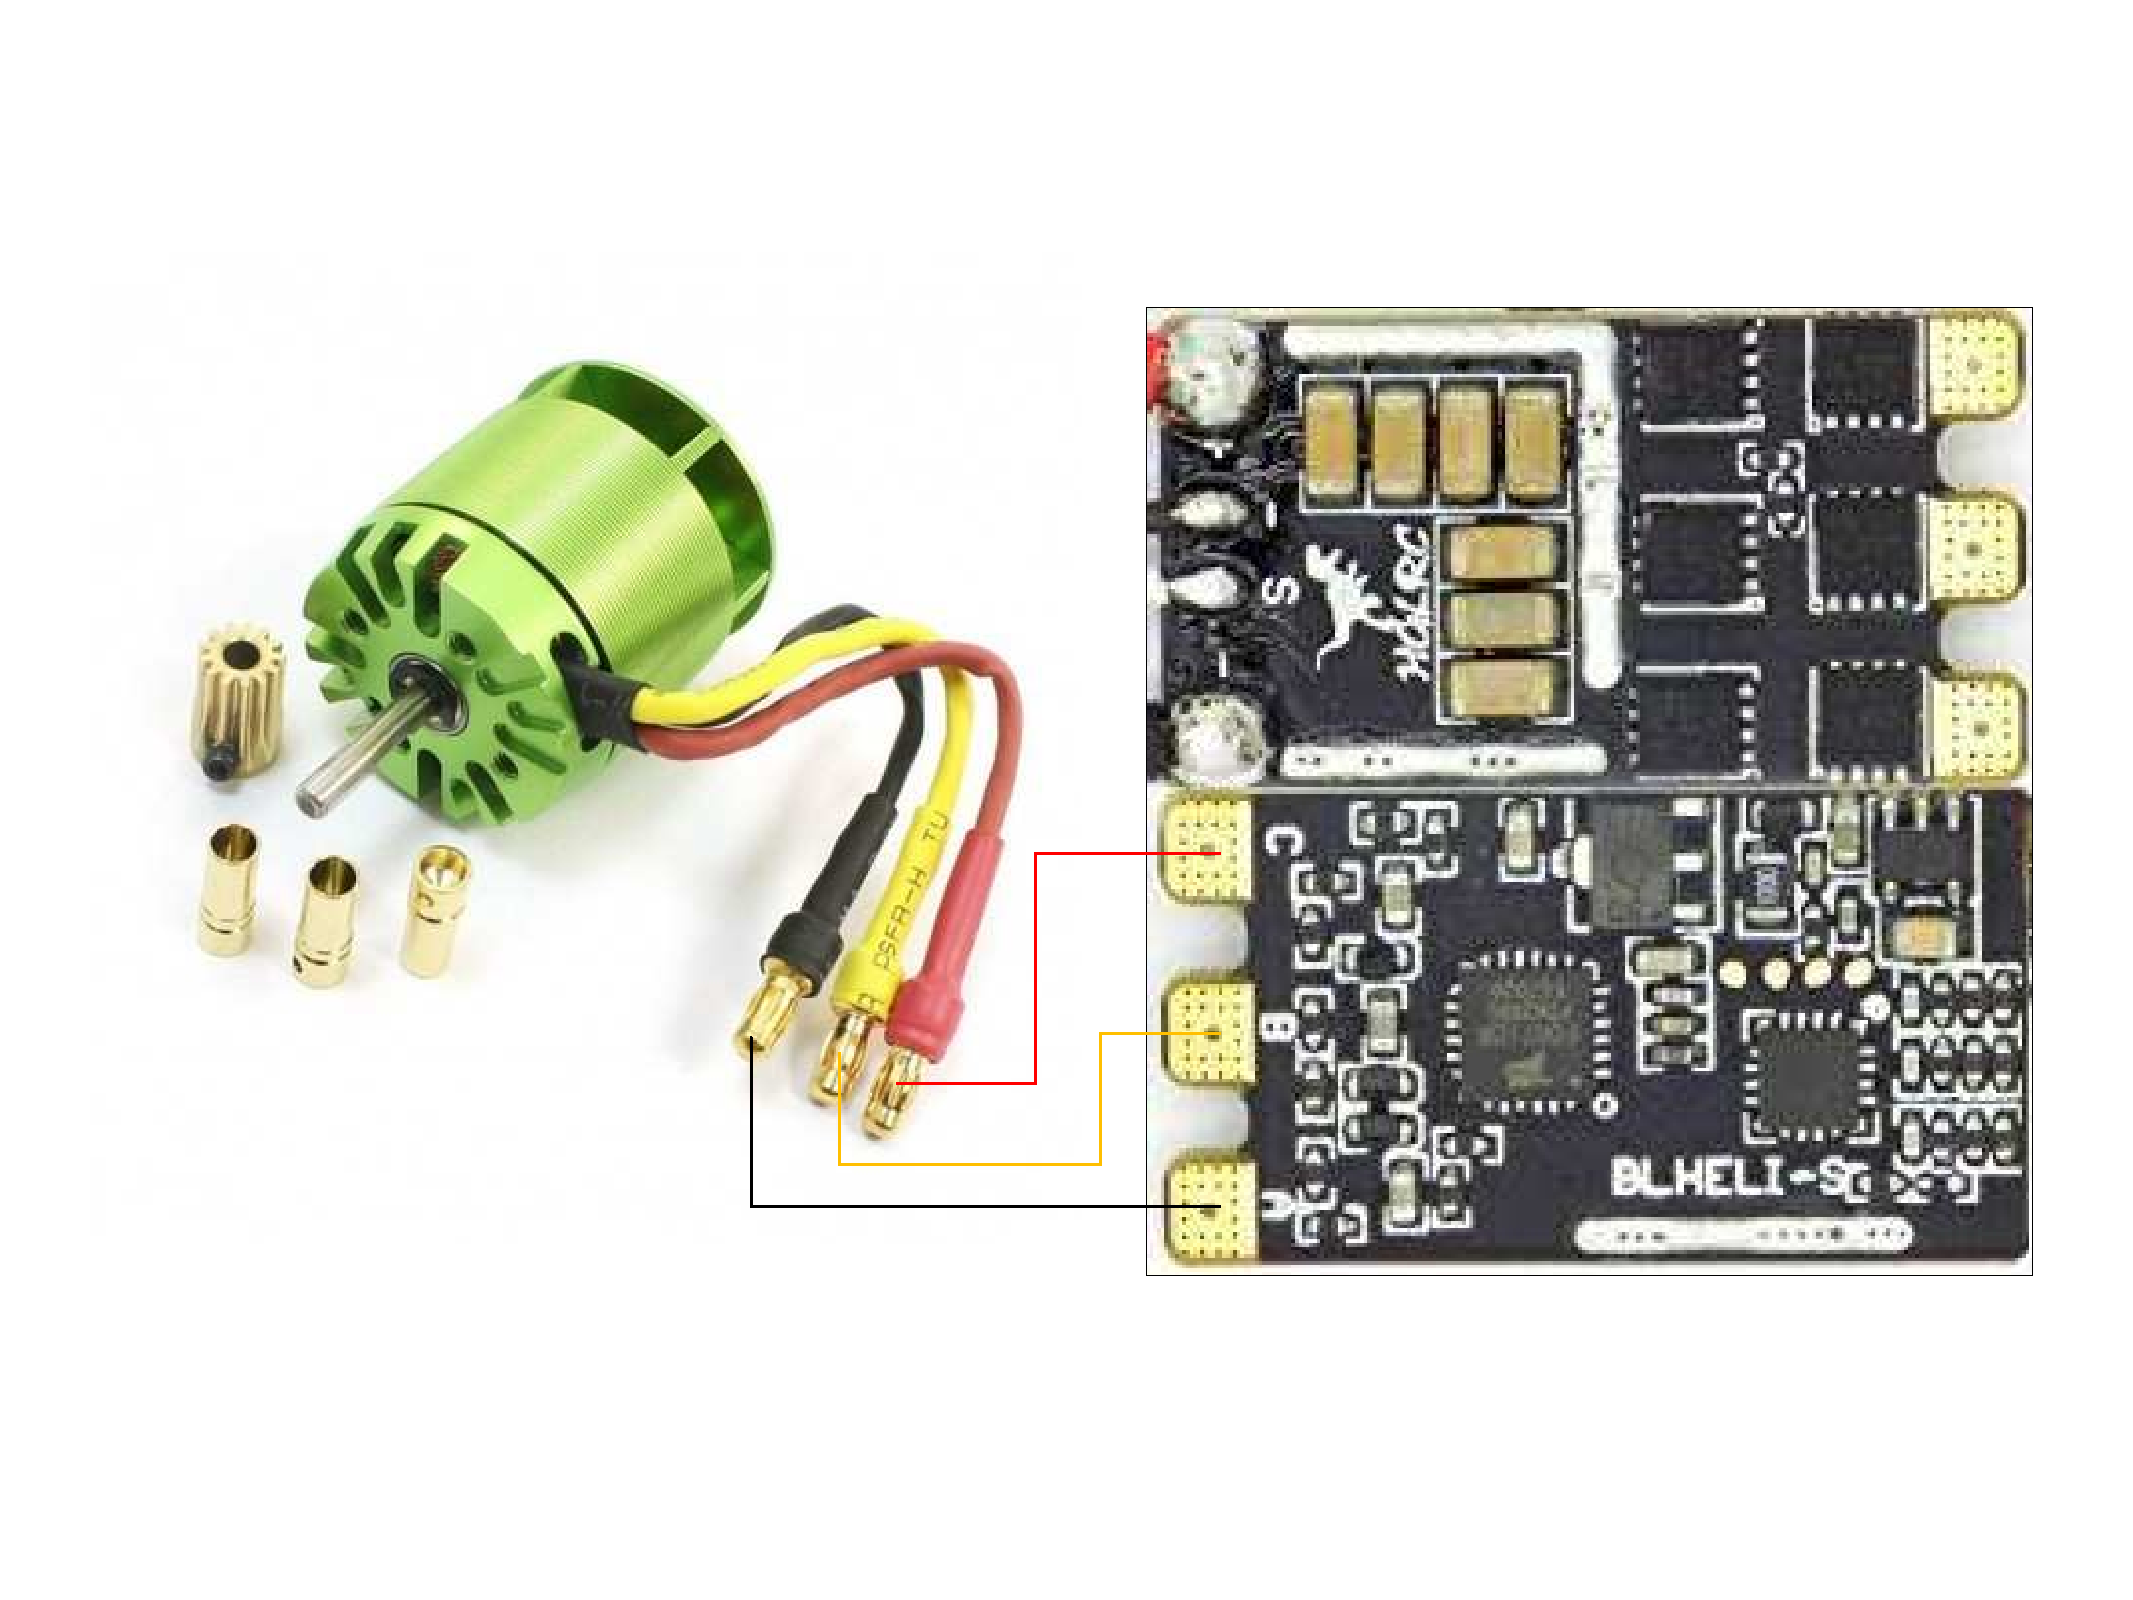
\includegraphics[width=8cm]{pictures/motor.pdf}
	\caption{Schéma zapojení motoru a regulátoru}
\end{figure}

\section{IMU}
IMU je zařízení, které měří úhlové rychlosti, zrychlení a orientaci v magnetickém poli ve třech osách. Skládá se z gyroskopu, akcelerometru  magnetometru. Všechny tři zařízení dohromady tvoří devět stupňů volnosti.  Použité IMU má shodný souřadný systém akcelerometru a gyroskopu, magnetometr má opačnou osu z a prohozené osy x a y.\cite{imu}\\

\subsection{Akcelerometr}
Akcelerometr slouží k určování zrychlení. Elektronický akcelerometr měří zrychlení na základě změny odporu mezi pevnou částí a pohyblivou částí akcelerometru. \\

\subsection{Gyroskop}
Gyroskop slouží k měření úhlové rychlosti.  Elektronický gyroskop měří úhlové rychlosti také na základě změny odporu, ale změnu měří ve dvou směrech na sobě kolmých. Z těchto dvou změn se vypočte úhel stočení.\\

\subsection{Magnetometr}
Magnetometr slouží k určování sil magnetického pole Země. Elektronický magnetometr využívá Hallův efekt, kdy vodivý plát je zasazen do elektronického obvodu. Při vlivu magnetického pole se na stranách plánu hromadí elektrony a protony, tomuto jevu se říká Hallův. Měřené napětí na stranách plátu je úměrné k síle magnetického pole.\\

%https://www.youtube.com/watch?v=eqZgxR6eRjo&t=149s

\textbf{Parametry použité IMU jednotky}\\
Arduino modul MPU9250\\
Obsahuje: akcelerometr, gyroskop, magnetometr\\
Komunikace: I2C, SPI\\
Vstup: VCC (5V), GND\\
Výstup: SDA, SCL (I2C)\\
Cena: 300 Kč\\
\cite{mpu9250}\\
%https://www.invensense.com/wp-content/uploads/2015/02/PS-MPU-9250A-01-v1.1.pdf
%mpu9250
\begin{figure}[H]
	\centering
	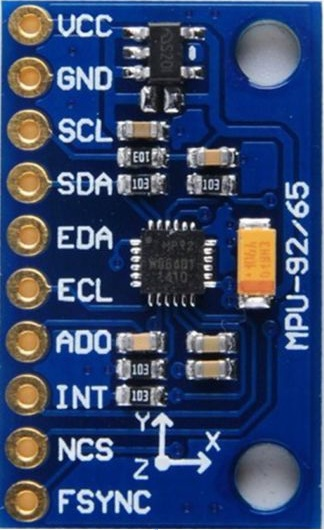
\includegraphics[width=3cm]{pictures/imu.jpg}
	\caption{IMU - MPU9250}
\end{figure}
 
\section{Komunikační zařízení} 
Pro bezdrátové ovládání dronu byl použit radiový modul a bluetooth.\\
\subsection{Radio} 
Radiový modul je používán pro zvětšení dosahu ovládání dronu. Pro stavbu byl použit bezdrátový modul XBee od firmy Digi. Modul plní funkce koncového zařízení, routeru nebo koordinátoru. Komunikace s XBee probíhá přes seriové rozhraní UART. Modul lze použít i pro čtení analogových a digitálních signálů různých senzorů.\\

\textbf{Parametry použitého Radiového zařízení}\\
XBEE PRO SS\\
Provozní napětí: 3.3V\\
Provozní frekvence: 2.4GHz\\
Komunikační protokol: ZB ZigBee\\
Dosah:1.5 km\\
\cite{xbee}\\

%https://www.proto-pic.co.uk/user/products/large/08665-03-L__99538__33841.jpg
\begin{figure}[H]
	\centering
	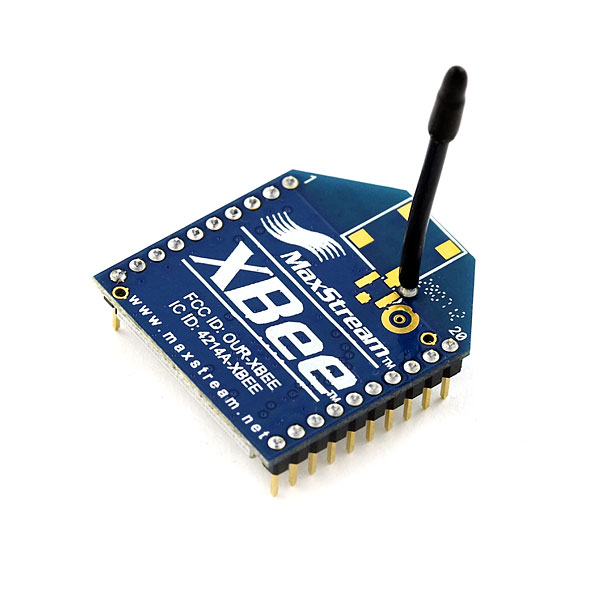
\includegraphics[width=5cm]{pictures/xbee.jpg}
	\caption{XBee}
\end{figure}

\subsection{Bluetooth} 
Pro bezdrátovou komunikaci s telefonem byl použit Arduino Bluetooth modul. Bluetooth modul využívá seriové rozhraní UART.\\

\textbf{Parametry použitého Bluetooth zařízení}\\
HC-05\\
Bluetooth verze: 2.0\\
Výchozí rychlost komunikace: 9600 baudů\\
Vstup: VCC (5V), GND, RX, EN\\
Výstup: TX, STATE\\
Použitá knihovna: SoftwareSerial\\
Cena: 200 Kč\\

\begin{figure}[H]
	\centering
	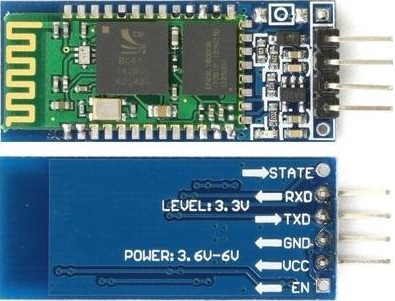
\includegraphics[width=5cm]{pictures/blue.jpg}
	\caption{Bluetooth - HC-05}
\end{figure}

\section{Řídící jednotka} 
Pro ovládání všech kompoment byla použita platforma Arduino.

\subsection{Arduino} 
Arduino je otevřená vývojová platforma, která využívá mikroprocesory od firmy Atmel. Programovat Arduino lze přes jazyk C nebo C++. Pro začínající uživatele byla vytvořena knihovna Wiring, která je velmi rozšířená. Knihovna je integrovaná do vývojového prostředí Arduino IDE. Na trhu existuje spousta typů desek např. Uno, Nano, Mega, Due. \\
Arduino lze napájet přes 12V konektor, USB nebo VIN, vstupní napětí je v rozsahu 5V - 12V. Vstupy Arduina jsou analogové, nebo digitální. Rozsah analogových vstupů je 0-1023. Digitální vstupy mají hodnotu LOW nebo HIGH, přenos dat probíhá přes PWM, I2C, SPI nebo UART komunikaci. Pro každou komunikaci jsou definovány určité digitální piny.\\

\textbf{Použité desky Arduino}\\
Arduino Uno\\
Arduino Nano\\
Arduino Due\\
Cena: 200 - 1000 Kč\\

\begin{figure}[H]
	\centering
	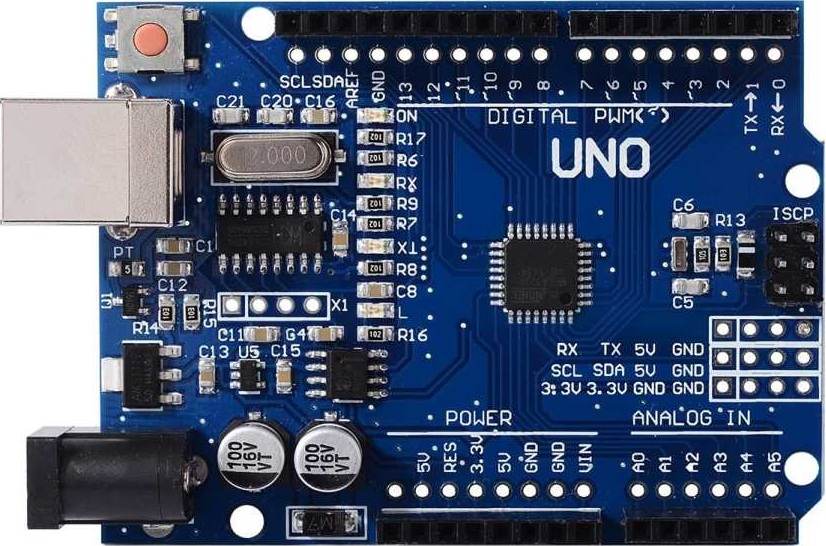
\includegraphics[width=5cm]{pictures/uno.jpg}
	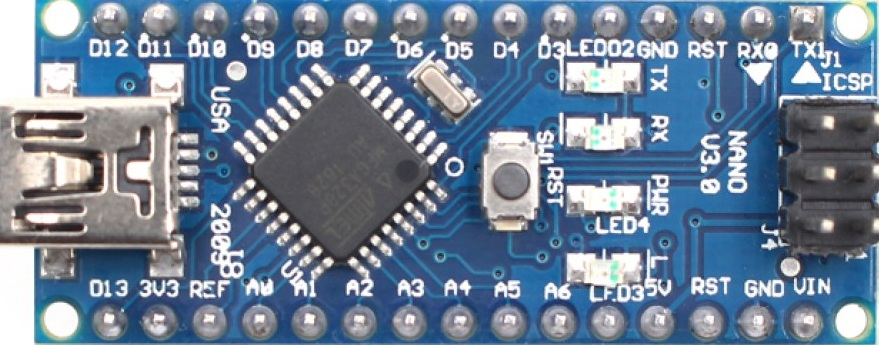
\includegraphics[width=5cm]{pictures/nano.jpg}
	\caption{Arduino UNO a Nano}
\end{figure}

\section{GNSS}
Při konstrukci měla být použita GNSS aparatura s podporou RTK z diplomové práce Štěpána Hodíka. Bohužel vzhledem problémům není GNSS aparatura zatím implementována.


\section{Výškoměr}
Pro funkci výškoměru byla požita dvě zařízení: barometr a GNSS.

\subsection{Barometr}
Barometrem měříme tlak a z rozdílů tlaků na starotvním místě a ve vzduchu lze zpočítat výška letu dronu.\\

\textbf{Použitý barometr}\\
BMP280\\
Vstup: VCC (3.3V), GND,\\
Výstup: SDA, SCL, SDO, CSB\\
Měřící rozsah teploty:-40 až +85 stupňů\\
Měřící rozsah tlaku:300 až 1100 hPa\\
Přesnost měření teploty: +- 1 stupeň\\
Přesnost měření tlaku:  +- 100 Pa\\
Použitá knihovna: Adafruit BMP280\\
Cena: 80 Kč\\
\cite{bpm}\\
%https://github.com/adafruit/Adafruit_BMP280_Library

\begin{figure}[H]
	\centering
	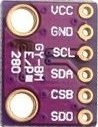
\includegraphics[width=2cm]{pictures/baro.jpg}
	\caption{Barometr - BMP280}
\end{figure}

\section{Laserový dálkoměr}
Pro automatizaci je důležité opatřit dron senzory měřící vzdálenosti pro detekci překážek. Senzory byly připevněny na ramena vrtulí pro měření vzdáleností ve vodorovné rovině a pro měření ve svislém směru pro přistávání a detekce objektů pod dronem. Použitý laserový dálkoměr měří vzdálenost pomocí tranzitního času.\\

\textbf{Použíty laserový modul}\\
laserový modul Vl53l0x\\
Vstup: VCC (5V), GND, XSHUT, GPIO1\\
Výstup: SDA, SCL (I2C)\\
vlnová délka: 940 nm\\
měřící rozsah: 0 - 1200 mm\\
přesnost: 3 procenta měřené délky\\
Použitá knihovna: VL53L0X\\
Cena: 230 Kč\\
\cite{laser}\\
%https://github.com/pololu/vl53l0x-arduino

\begin{figure}[H]
	\centering
	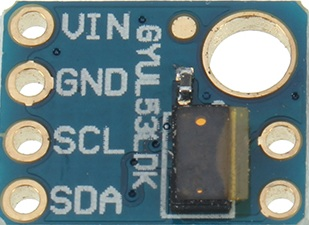
\includegraphics[width=2cm]{pictures/laser.jpg}
	\caption{Laserový modul - Vl53l0x}
\end{figure}

Při používání pouze jednoho modulu stačí propojit pouze 4 pin VIN, GND, SCL, SDA. Pro více modulů je potřeba zapojit pin XSHUT na některý z digitálních pinů. Pin XSHUT slouží k přepnutí modulu do stan-by režimu, pro definování adresy, přes I2C komunikaci, na používaném modulu.

\section{Kamera}
Pro obrazový vjem letu dronu byl nainstalován systém FPV. FPV se skládá z kamery, vysílače, přijímače a obrazového media. Kamera předává obrazová data radiovému vysílači, který je na určité frekvenci posílá přijímači. Přijímač signál dekóduje a zobrazí na mediu.\\

\textbf{Použítá kamera}\\
Eachine TX02\\
Vstup: VCC (5V), GND\\
Výstup: radiový signál s frekvencí 5.8GHz\\
Zorné pole: 120 stupňů\\
Rozlišení: 600TVL\\
Použitá Android aplikace: FPViewer\\
Cena: 800 Kč\\

\begin{figure}[H]
	\centering
	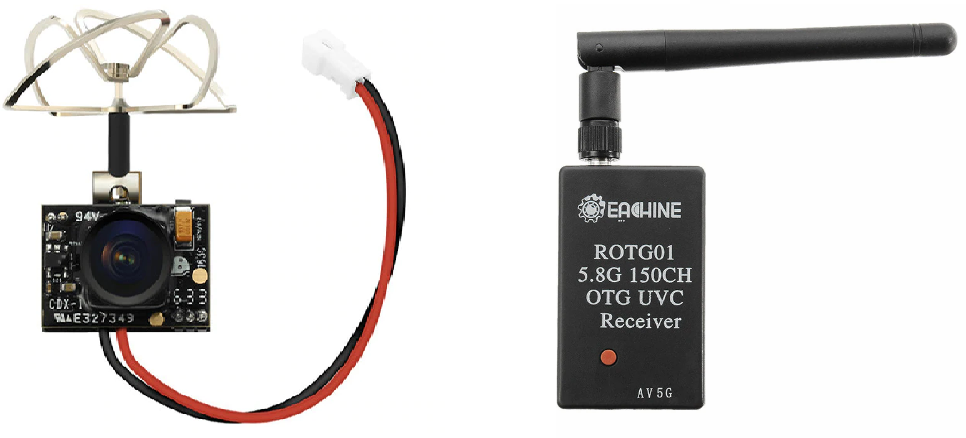
\includegraphics[width=10cm]{pictures/camera.png}
	\caption{Kamera TX02 s přijímačem pro smartphone}
\end{figure}
%\chapter{Stavba}
\label{4-stavba}
\chapter{Konstrukce}
\label{4-algoritmus}

\section{Ovládání ESC (regulátorů otáček)}
Regulátor je ovládán přes různé komunikační protokoly. Komunikační protokoly jsou buď analogové nebo digitální. Mezi analogové protokoly patří standartní PWM signál, OneShot125, OneShot42 a MultiShot, mezi digitální patří  DSHOT300, DSHOT600 a DSHOT1200. \cite{comregul}\\
Standartní PWM signál není klasický PWM signál, kterým se například reguluje výkon žárovky. Standartní PWM signál definuje nulový výkon motoru pro pulz o délce 1ms a maximální výkon o délce 2ms. Teoretická frekvence je 500Hz, lze tedy měnit rychlost motorů 500krát za vteřinu.\\
Ostatní protokoly jsou sice rychlejší, ale nemá smysl je implementovat na platformu Arduino z důvodu malého výkonu platformy.\\ 

\begin{table}[H]
\centering
	\begin{tabular}{|l|l|l|l|}
		\hline
		\textbf{Protokol} & \textbf{Frekvece} & \textbf{Min pulz} & \textbf{Max pulz} \\ \hline
		Standart PWM      & 500 Hz            & 1000 µs            & 2000 µs            \\ \hline
		OneShot125        & 4 kHz             & 125 µs             & 250 µs             \\ \hline
		OneShot42         & 12 kHz            & 42 µs              & 84 µs              \\ \hline
		MultiShot         & 40 kHz            & 12.5 µs            & 25 µs              \\ \hline
	\end{tabular}
\caption{Analogové komunikační protokoly pro regulátory otáček}
\end{table}

\begin{table}[H]
	\centering
	\begin{tabular}{|l|l|}
		\hline
		\textbf{Protokol} & \textbf{Rychlost komunikace} \\ \hline
		DSHOT150          & 150 000 bps                  \\ \hline
		DSHOT300          & 300 000 bps                  \\ \hline
		DSHOT600          & 600 000 bps                  \\ \hline
		DSHOT1200         & 1200 000 bps                 \\ \hline
	\end{tabular}
\caption{Digitální komunikační protokoly pro regulátory otáček}
\end{table}

\textbf{PWM}\\
PWM modulace je určená pro přenos analogového signálu pomocí dvou hodnot (Low a High), přenos probíhá na digitálních pinech. Přenášená hodnota je zaimplementována do poměru High/Low. Poměr se nazývá střída a nabývá hodnot 0-100 procent. Hodnoty Low a High se zapisují v cyklu.\cite{pwmwiki}\\


%http://1oomzzme3s617r8yzr8qutjk-wpengine.netdna-ssl.com/wp-content/uploads/2017/04/Fig-1-pwm.gif
%pwm
\begin{figure}[H]
	\centering
	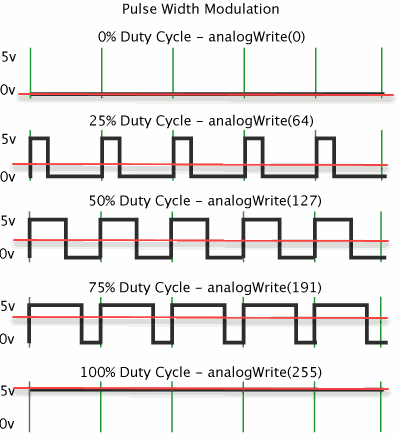
\includegraphics[width=10cm]{pictures/pwm.png}
	\caption{Ukázka PWM}
	\cite{pwm}\\
\end{figure}


\section{Kalibrace regulátorů otáček}
%https://www.youtube.com/watch?v=61bjFxJyOLU&t=52s
%blheli
Kalibrace regulátorů je nutná pro definování komunikačního protokolu a různých funkcí.\\
Pro kalibraci je potřeba kalibrovaný regulátor, propojovací dráty a Arduino Nano. V programu BLHeliSuite lze kalibrovat i s jinou platformou Arduino, bohužel kalibrace se podařila pouze s deskou typu Nano. Zapojení regulátoru se provede přes schéma na obrázku 5.2.\\
Po zapojení komponent a nastavení šablony se vybere sériový port pro komunikaci mezi počítačem a Arduinem. Přes tlačítko Read Setup se načte tovární nastavení regulátoru.\cite{blheli}\\
\begin{figure}[H]
	\centering
	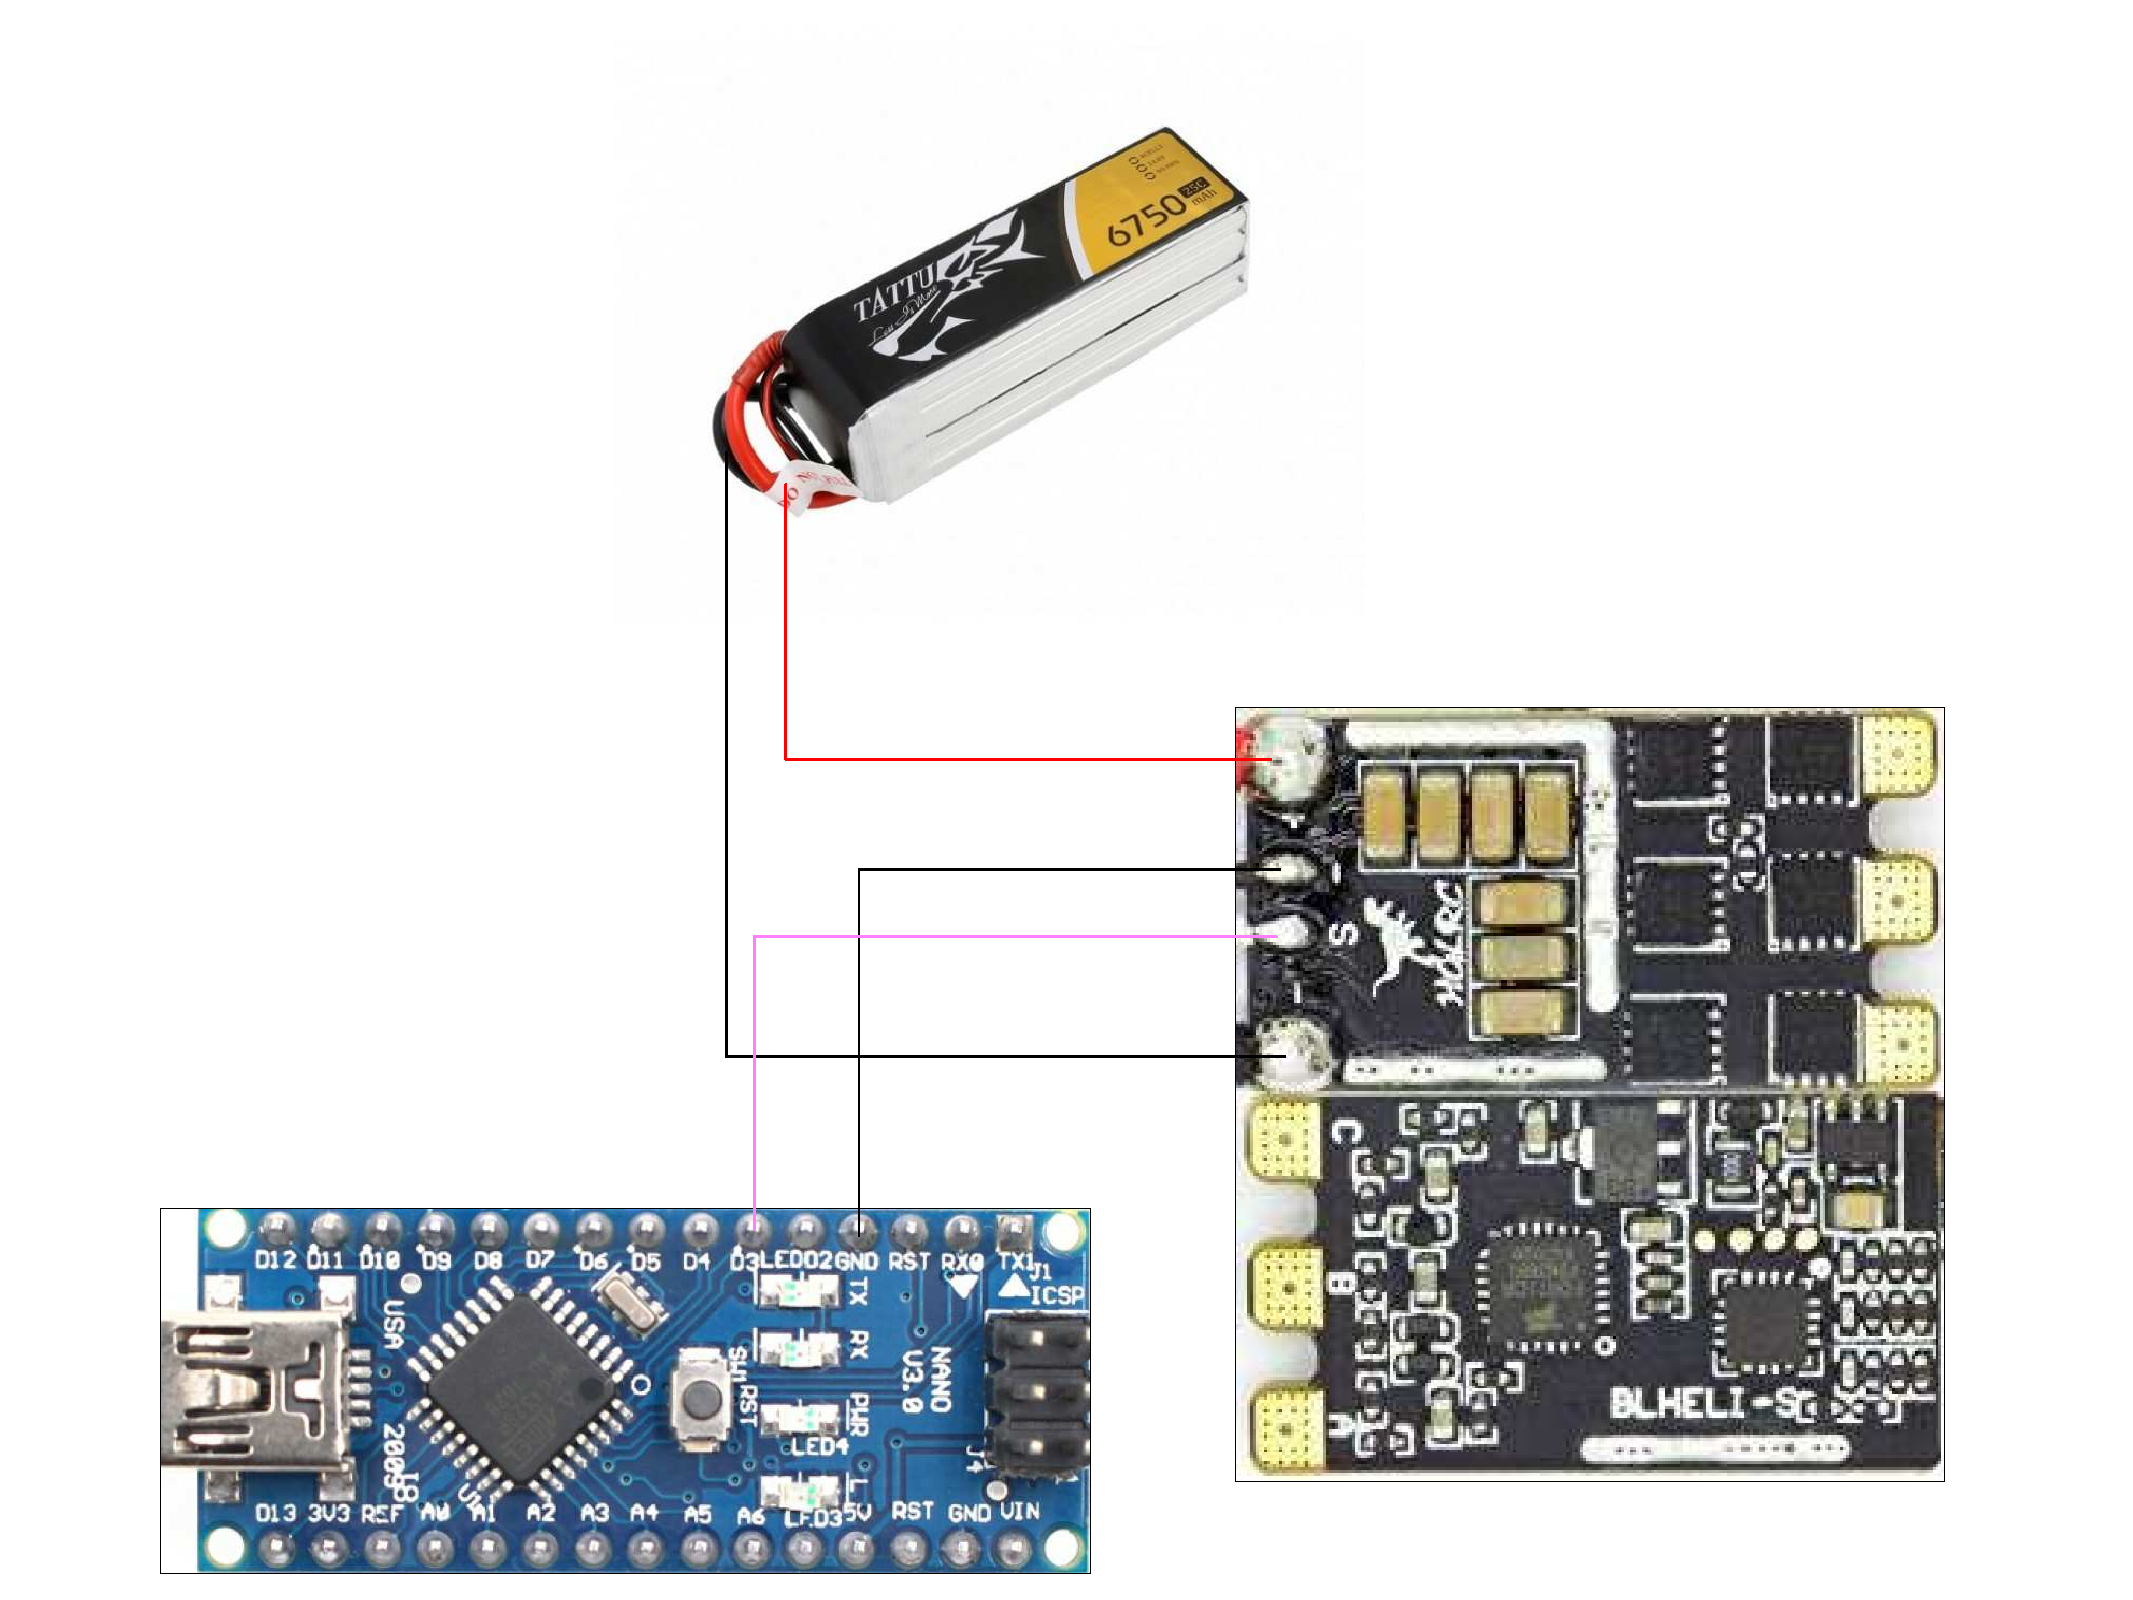
\includegraphics[width=12cm]{pictures/esc_calib.pdf}
	\caption{Schéma zapojení pro kalibraci regulátoru otáček}
\end{figure}
Nastaví se PPM Min Throttle hodnota na 1000, PPM Max Throttle na 2000 a PPM Center Throttle na 1500. Zapíše se hodnota do regulátoru. Výsledkem jsou zkalibrované vstupní hodnoty pulzu do intervalu <1000;2000>. PPM je jiný typ modulace než PWM, k ovládání regulátorů otáček stačí znát pouze PWM modulaci.\\

\begin{figure}[H]
	\centering
	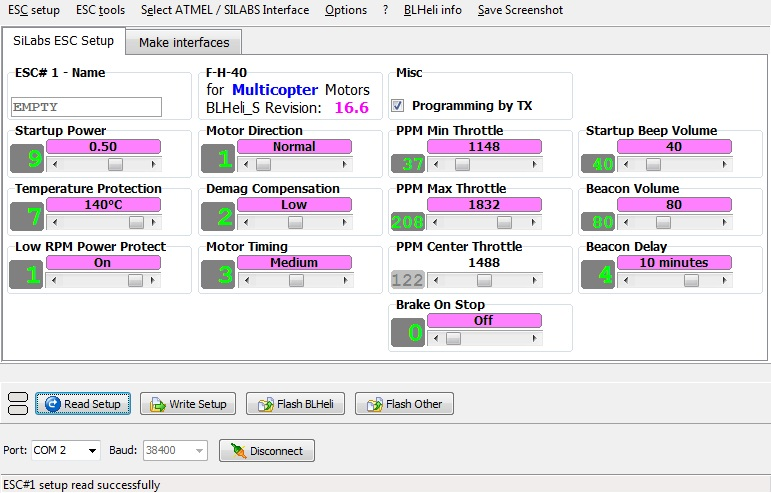
\includegraphics[width=12cm]{pictures/esc_calib5.jpg}
	\caption{Ukázka kalibrace v programu HLBeliSuite před kalibrací}
\end{figure}

\begin{figure}[H]
	\centering
	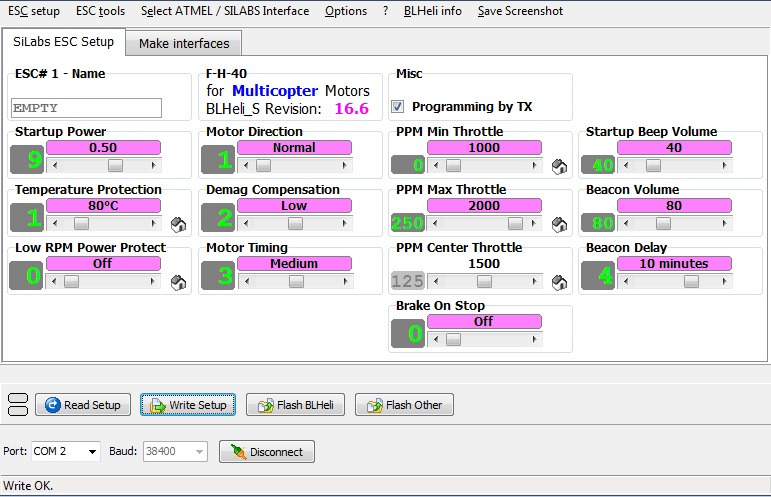
\includegraphics[width=12cm]{pictures/esc_calib6.jpg}
	\caption{Ukázka kalibrace v programu HLBeliSuite po kalibraci}
\end{figure}

\section{Filtrace dat IMU}
\textbf{Výpočet úhlů pitch a roll z dat akcelerometru.}\\
\begin{eqnarray*} 
	pitchAcc & = & atan2 (yAcc , \sqrt{xAcc^{2} + zAcc^{2}})\\
	rollAcc & = & atan2 (xAcc , \sqrt{yAcc^{2} + zAcc^{2}})\\
\end{eqnarray*} 
\textbf{Výpočet úhlů pitch a roll z dat gyroskopu}\\
Jelikož gyroskop měří úhlovou rychlost, úhly pitch a roll jsou určeny integrací z počátečního stavu. Pokud IMU jednotka nebude v počátečním stavu ve vodorovné poloze, úhly pitch a roll nebudou absolutní.\\
\begin{eqnarray*} 
	pitchGyro & = & pitchGyro + xGyro * dt\\
	rollGyro & = & rollGyro + yGyro * dt\\
	yawGyro & = & yawGyro + zGyro * dt\\
\end{eqnarray*} 
\textbf{Výpočet úhlů yaw z dat magnetometru.}\\
Při výpočtu úhlu yaw z dat magnetometru je nutné zahrnout magnetickou deklinaci, které je závislá na zeměpisných souřadnicích. \cite{declination}\\
\begin{eqnarray*} 
	yawMag & = & atan2(yMag, xMag)+ declinationMag\\
\end{eqnarray*} 

Surová data ze všech tří senzorů nejsou použitelná pro výpočet úhlů náklonu, obsahují nepřesnosti a šum, proto je potřebná filtrace.\\

%https://aip.scitation.org/doi/pdf/10.1063/1.5018520

\subsection{Komplementární filtr}
Komplementární filtr je nejjednodušší z uvedených filtrů. Využívá data z akcelerometru a gyroskopu. \\
Z dlouhodobého hlediska data z gyroskopu konvergují. Z krátkodobého hlediska jsou přesná, proto je potřeba použít High Pass filtr.\\
Opakem toho jsou data z akcelerometru, data jsou ovlivňována malými silami, které ruší výsledné zrychlení. Z dlouhodobého hlediska jsou data z akcelerometru přesná, proto je potřeba použít Low Pass filtr.\\
Kombinací High Pass filtru a Low Pass filtru vzniká komplementární filtr, který je pro ovládání dronu dostačující.\\
\begin{figure}[H]
	\centering
	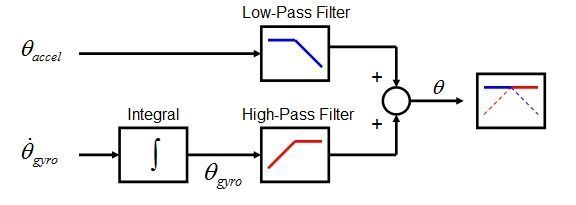
\includegraphics[width=15cm]{pictures/complementary.jpg}
	\caption{Schéma Komplementárního filtru}
	\cite{complementary}
\end{figure}
\begin{eqnarray*} 
	pitch & = & 0.996 * (pitch + xGyro * dt) + 0.004 * pitchAcc\\
	roll & = & 0.996 * (roll + yGyro * dt) + 0.004 * rollAcc\\
\end{eqnarray*}


\subsection{Kalmanův filtr}
Kalmanův filtr je dynamický filtr, který pracuje s predikcí. Pro výpočet je potřeba stanovit model systému, u kterého bude filtr predikovat stavy. Pokud v oblasti predikovaného stavu najdeme skutečný stav, provede se korekce skutečného stavu a oblast predikovaného stavu bude menší/přesnější. Není-li nalezen skutečný stav v oblasti predikovaného stavu, oblast predikovaného stavu se zvětší a tím se zhorší přesnost výpočtu.\\
Bohužel Kalmanův filtr nemohl být použit z důvodu malého výpočetního výkonu platformy Arduino.

\subsection{Mahonyho filtr}
Mahonyho filtr využívá Quaternions, což je čtyř dimenzionální numerický systém využívaný pro popis rotace objektu v počítačové grafice a robotice. Filtr používá data z gyroskopu, akcelerometru a magnetometru, přičemž z nich počítá úhly pitch, roll a yaw. Při výpočtu byla použita knihovna MahonyAHRS. \cite{mahony}\\
%https://github.com/PaulStoffregen/MahonyAHRS
%https://www.youtube.com/watch?v=zjMuIxRvygQ

\section{PID regulátor pro synchronizaci motorů} 
PID regulátor slouží k regulaci požadovaného stavu v nejkratší době a to pomocí zvyšování a snižování vlivu, který napomáhá dostat se do požadovaného stavu.\\
Názorný příklad:
Požadujeme, aby dron držel stabilní polohu. Chceme, aby úhly pitch a roll z IMU byly nulové. Kdybychom měli ideální dron s přesným vyvážením hmotnosti a se stejně fungujícími motory, bylo by to snadné. Pouze by stačilo zapsat stejnou hodnotu na všech motorech a dron by bez problémů vzlétnul. Bohužel ideální dron nemáme, proto motory musí být ovládany individuálně. PID regulátor počítá výkon motoru v závislosti na rozdílu skutečných úhlů od požadovaných.\\
PID regulátor reaguje na tzv. errory (odchylky od požadovaného stavu) a následně přes koeficienty kp, ki a kd spočte hodnoty pro ovládání motorů.
PID regulátor má tři složky: proporcionální (kp), integrační (ki) a derivační (kd).\\
Proporcionální složka ovlivňuje výkon motoru lineárně. Pokud existuje odchylka zvýší se výkon motorů. Pokud je odchylka nulová, proporcioální složka neovlivňuje výkon motorů.\\
Integrační složka ovlivňuje výkon motorů v závislosti na předchozím stavu. Pokud dron není v požadovaném stavu, integrační složka se zvyšuje, dokud není dosažen požadovaný stav.\\
Derivační složka reaguje na změnu rychlosti odchylky. Čím rychleji se bude odchylka měnit, tím větší bude vliv derivační složky. Derivační složka reaguje proti P a I složce.\\
Pro autonomní řízení dronu je potřeba celkem šest PID regulátorů viz obr. 5.7. Základem jsou tři PID regulátory pro úhly pitch, roll a yaw. S těmito třemi regu\-látory, lze létat s dronem přes manuální ovládání. Kontrolu  nad těmito regulátory obstarává letový kontrolér (flying controller).\\
Navigační kontrolér (navigation controller) ovládá další tři regulátory. PID regulátor výkonu (throttle) reaguje na nadmořskou výšku dronu, reguluje konstatní výkon všech motorů pro let ve výšce zadané uživatelem. PID regulátory pro roll a pitch korigují směr letu dronu v závislosti na jeho poloze měřenou GNSS aparaturou.\cite{pid} \cite{hacksterpid}\\
\begin{figure}[H]
	\centering
	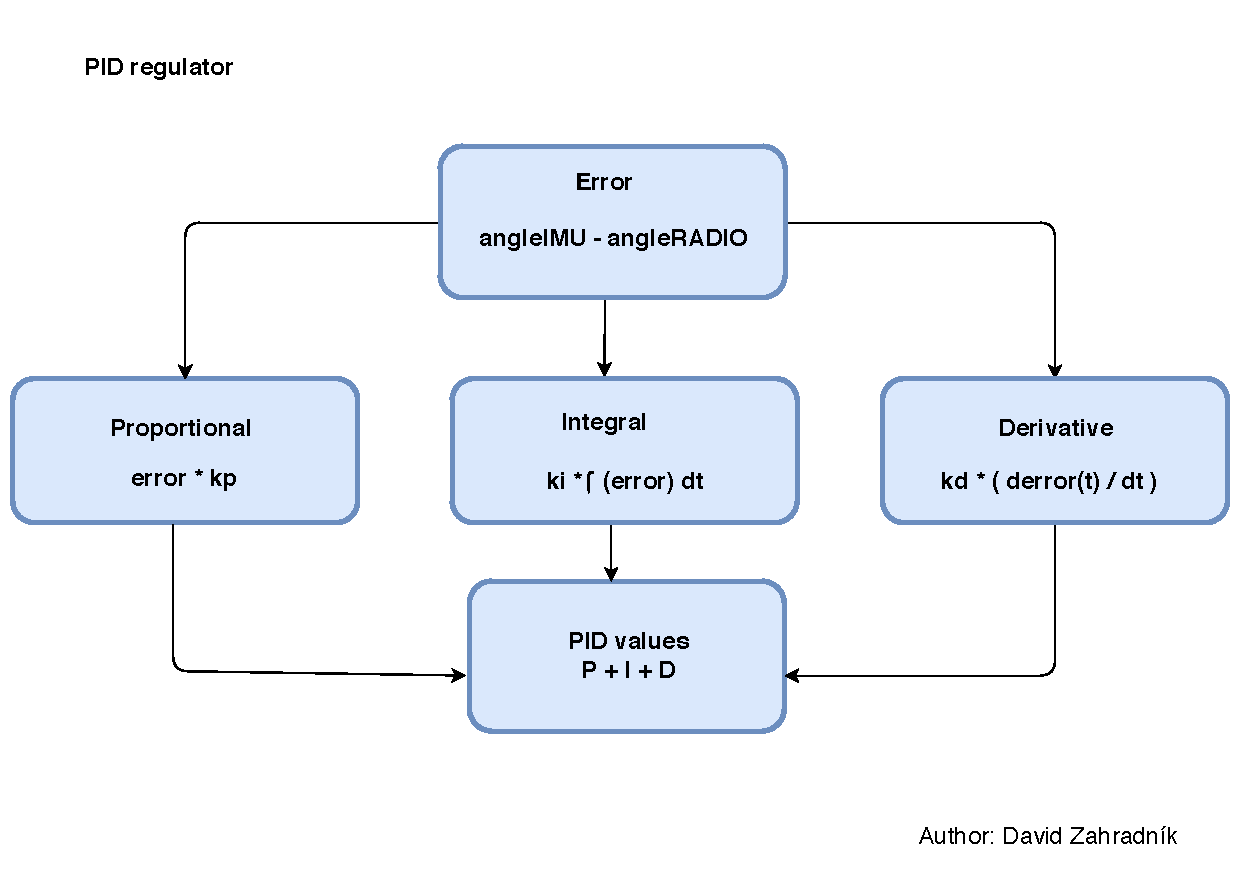
\includegraphics[width=15cm]{pictures/PIDDiagram.pdf}
	\caption{Schéma PID regulátoru}
\end{figure}
\begin{figure}[H]
	\centering
	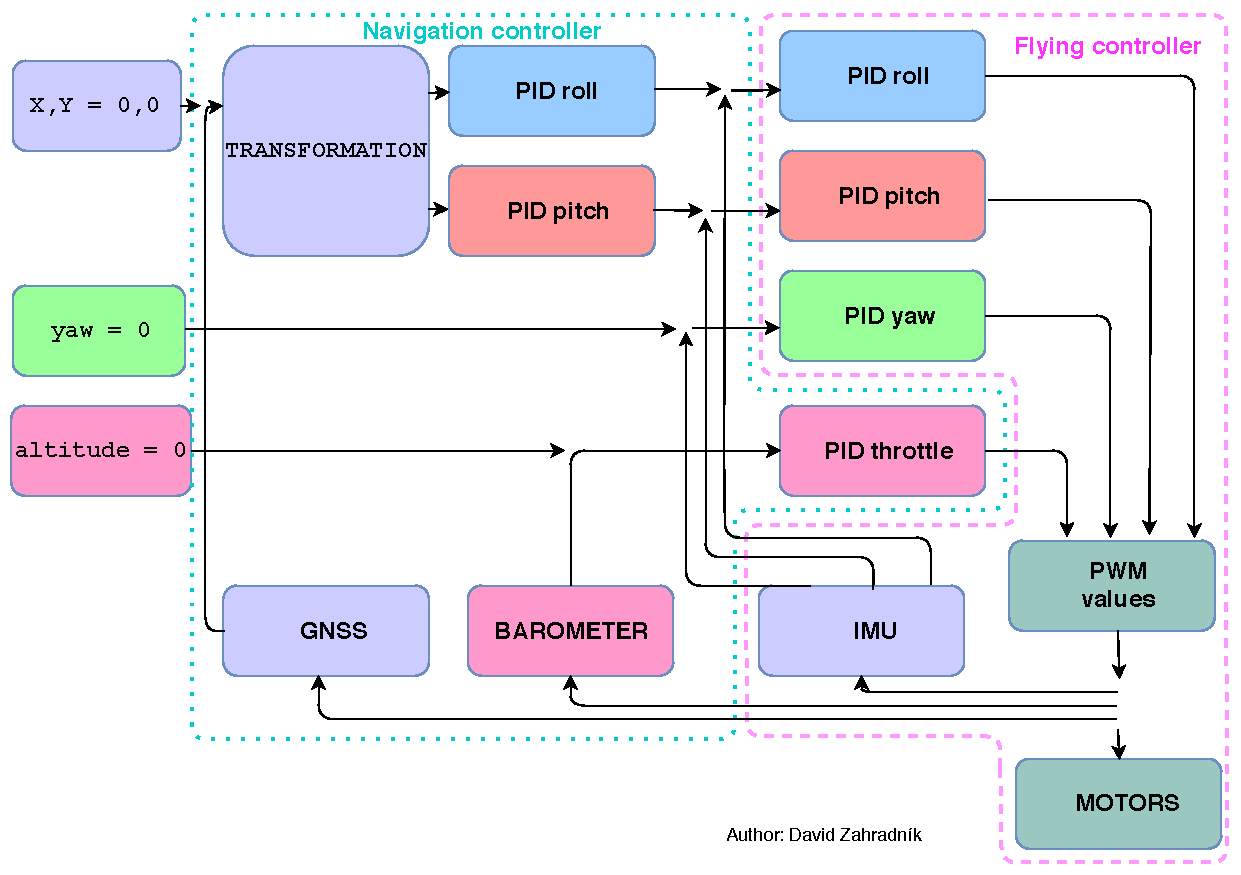
\includegraphics[width=15cm]{pictures/PIDsDiagram.pdf}
	\caption{Schéma všech PID regulátorů při stavbě dronu}
\end{figure}
%https://valter.byl.cz/plynula-regulace-pid
%pid
%http://www.controlengcesko.com/hlavni-menu/artykuly/artykul/article/derivacni-slozka-v-regulaci-pid/

\section{Komunikační protokol}
Pro propojení dronu a smartphonu je použita bluetooth a radiová komunikace. Komunikace je realizována přes sériové rozhraní UART, pro projení se používají piny RX a TX. UART lze implementovat pouze mezi dvěma zařízeními. Pro realizaci komunikace je nutné nastavit stejnou rychlost komunikace (bps).\\
Pro použití rozhraní UART byl vytvořen komunikační protokol pro ovládání dronu. Začátek zprávy je definován znakem < a konec zprávy >. Hodnoty potřebné pro ovládání jsou určeny prvním bytem (znakem) a hodnota následující dvěma byty. Hodnota dána čísly 0-99 se interpoluje do rozsahu uvedeného v tabulce.\\

\begin{table}[H]
	\centering
	\begin{tabular}{|l|l|l|l|}
		\hline
		\textbf{Znak} & \textbf{Typ hodnoty} & \textbf{Od} & \textbf{Do} \\ \hline
		T             & Výkon                & 1000 µS     & 1700 µS     \\ \hline
		P             & Pitch                & -25 $^\circ$        & +25 $^\circ$        \\ \hline
		R             & Roll                 & -25 $^\circ$        & +25 $^\circ$        \\ \hline
		Y             & Yaw                  & 0 $^\circ$          & 360 $^\circ$        \\ \hline
		D             & Stupně               & 48 (12) $^\circ$    & - 52 (15) $^\circ$  \\ \hline
		M             & Minuty               & 0 ´           & 60 ´         \\ \hline
		S             & Sekundy              & 0 ´´          & 60 ´´         \\ \hline
		C             & kalibrace            & null        & null        \\ \hline
		H             & návrat               & null        & null        \\ \hline
		F             & zem. šířka           & null        & null        \\ \hline
		L             & zem. délka           & null        & null        \\ \hline
	\end{tabular}
\caption{Komunikační protokol přes seriové rozhraní UART}
\end{table}

\section{Radiová komunikace XBEE}
Před zahájením komunikace mezi radiovými moduly je nutné provést jejich konfi\-guraci. Ke konfiguraci slouží program XCTU (Linux, Windows) od výrobců mo\-dulů XBEE. Pro propojení počítače a modulu lze použít shield (nadstavbové zařízení k mikrokontrolérům) od firmy Digi, nebo je možné využít platformu Arduino a \mbox{Arduino} XBEE shield.\\
K propojení radiového modulu a počítače s pomocí platformy Arduino, je nutno provést několik kroků. V první řadě je do platformy nahrán jednoduchý kód, který bude mít za úkol číst data z počítače a posílat je radiovému modulu. V kódu je třeba definovat, na kterých pinech bude prováděna komunikace s radiovým mo\-dulem. Druhý krok je nastavení pinů pro komunikaci s radiovým modulem na shieldu. V posledním kroku jsou dílčí součástky spojeny.\\
Nejdůležitějšími nastaveními radiových modulů jsou definování funkce, rychlost komunikace (bps) a ID sítě. V síti radiových modulů je potřeba jeden koordinátor, na počtu routerů a koncových zařízení nezáleží. Koordinátor obstarává inicializaci sítě a umožnuje dalším modulům připojení do sítě. Router funguje jako prostředník při přenosu dat. Koncové zařízení slouží buď k příjmu nebo odesílání zpráv. Rychlost komunikace je dána přenosem bitů za sekundu (bps) a musí být totožná na všech zařízeních v síti. ID sítě slouží k uzavření komunikace jenom mezi určitými radiovými moduly. \cite{xbeetut}\\\\
%https://www.tunnelsup.com/xbee-guide/
%xbeetut

\begin{figure}[H]
	\centering
	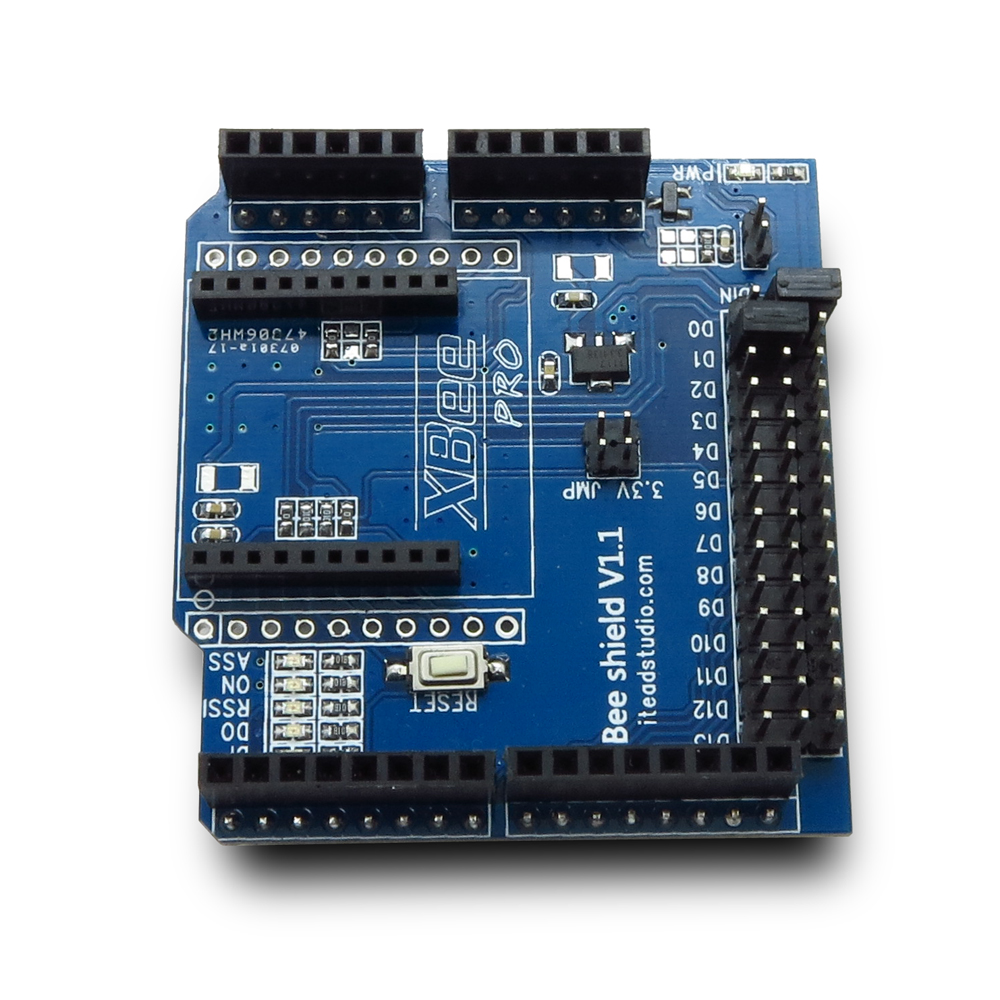
\includegraphics[width=8cm]{pictures/xbeeshield.jpg}
	\caption{XBEE shield}
\end{figure}


\section{Letový kontrolér} 
\textbf{Vstup:} IMU, Navigační kontrolér\\
\textbf{Výstup:} ESC\\
Letový kontrolér slouží k synchronizaci a ovládání motorů dronu. Letový kontrolér zpracovává měření z IMU a porovnává jej s daty z navigačního kontroléru (pitch, roll a yaw). Pokud úhly náklonů nejsou totožné, kontrolér přes PID regulátory změní výkon motorů tak, aby úhly ztotožnil.\\
Při spuštění letový kontrolér provede kalibraci regulátorů otáček zapsáním minimální a maximální hodnoty výkonu.\\
Po kalibraci regulátorů otáček, kontrolér čte data z IMU, probíhá filtrace pomocí komplementárního filtru a počítá úhly pitch, roll a yaw.\\
Z navigačního kontroléru jsou získávána data, která jsou následně separována a interpolována do požadovaných hodnot. Hodnoty jsou rozlišovány prvním bytem, který definuje o jakou hodnotu se jedná. Další dva byty představují číslo od 0 do 99, které je interpolováno na požadovaný rozsah.\\
Hodnota výkonu motoru/throttle se vyinterpoluje pouze do 1700 µS, protože ke konstantnímu výkonu jsou připočítávány údaje z PID regulátoru. Rozsah dat z PID regulátoru je <-300;300>, pokud by se zapsal konstaní výkon větší než 1700 µS, PID regulátor by byl omezen.\\
Hodnota náklonů pitch a roll  může být nejvýše 25 stupňů, kdyby byla hodnota větší, hrozilo by převrácení dronu.\\
Z rozdílu úhlů z IMU a navigačního kontroléru se vypočtou odchylky. Podle odchylek se vyčíslí proporcionální, integrační a derivační složka PID regulátoru každého úhlu. Součet všech tři složek představuje změnu výkonu motoru pro jednotlivý úhel. Dle pohybových rovnic jsou vypočteny výkony motorů.\\
Pro zápis výkonu motorů byl implementován komunikční protokol s frekvencí 250 Hz(viz obrázek 5.10), který výchází ze standartního PWM signálu. První fázi je prováden výpočet komplementárního filtru, výpočet hodnot PID regulátorů a čtení dat za navigačního kontroléru. Ve druhé fázi jsou čtena data z IMU jednotky a zapisovány hodnoty výkonu pro regulátory otáček(ESC). Doba trvání obou fázi jsou čtyči milisekundy, frekvence tedy je 250 Hz. V druhé fázi, kdy zapisování hodnot výkonu trvá jednu až dvě milisekundy, jsou pro úsporu času v první milisekundě čtena data z IMU jednotky.\\
\begin{figure}[H]
	\centering
	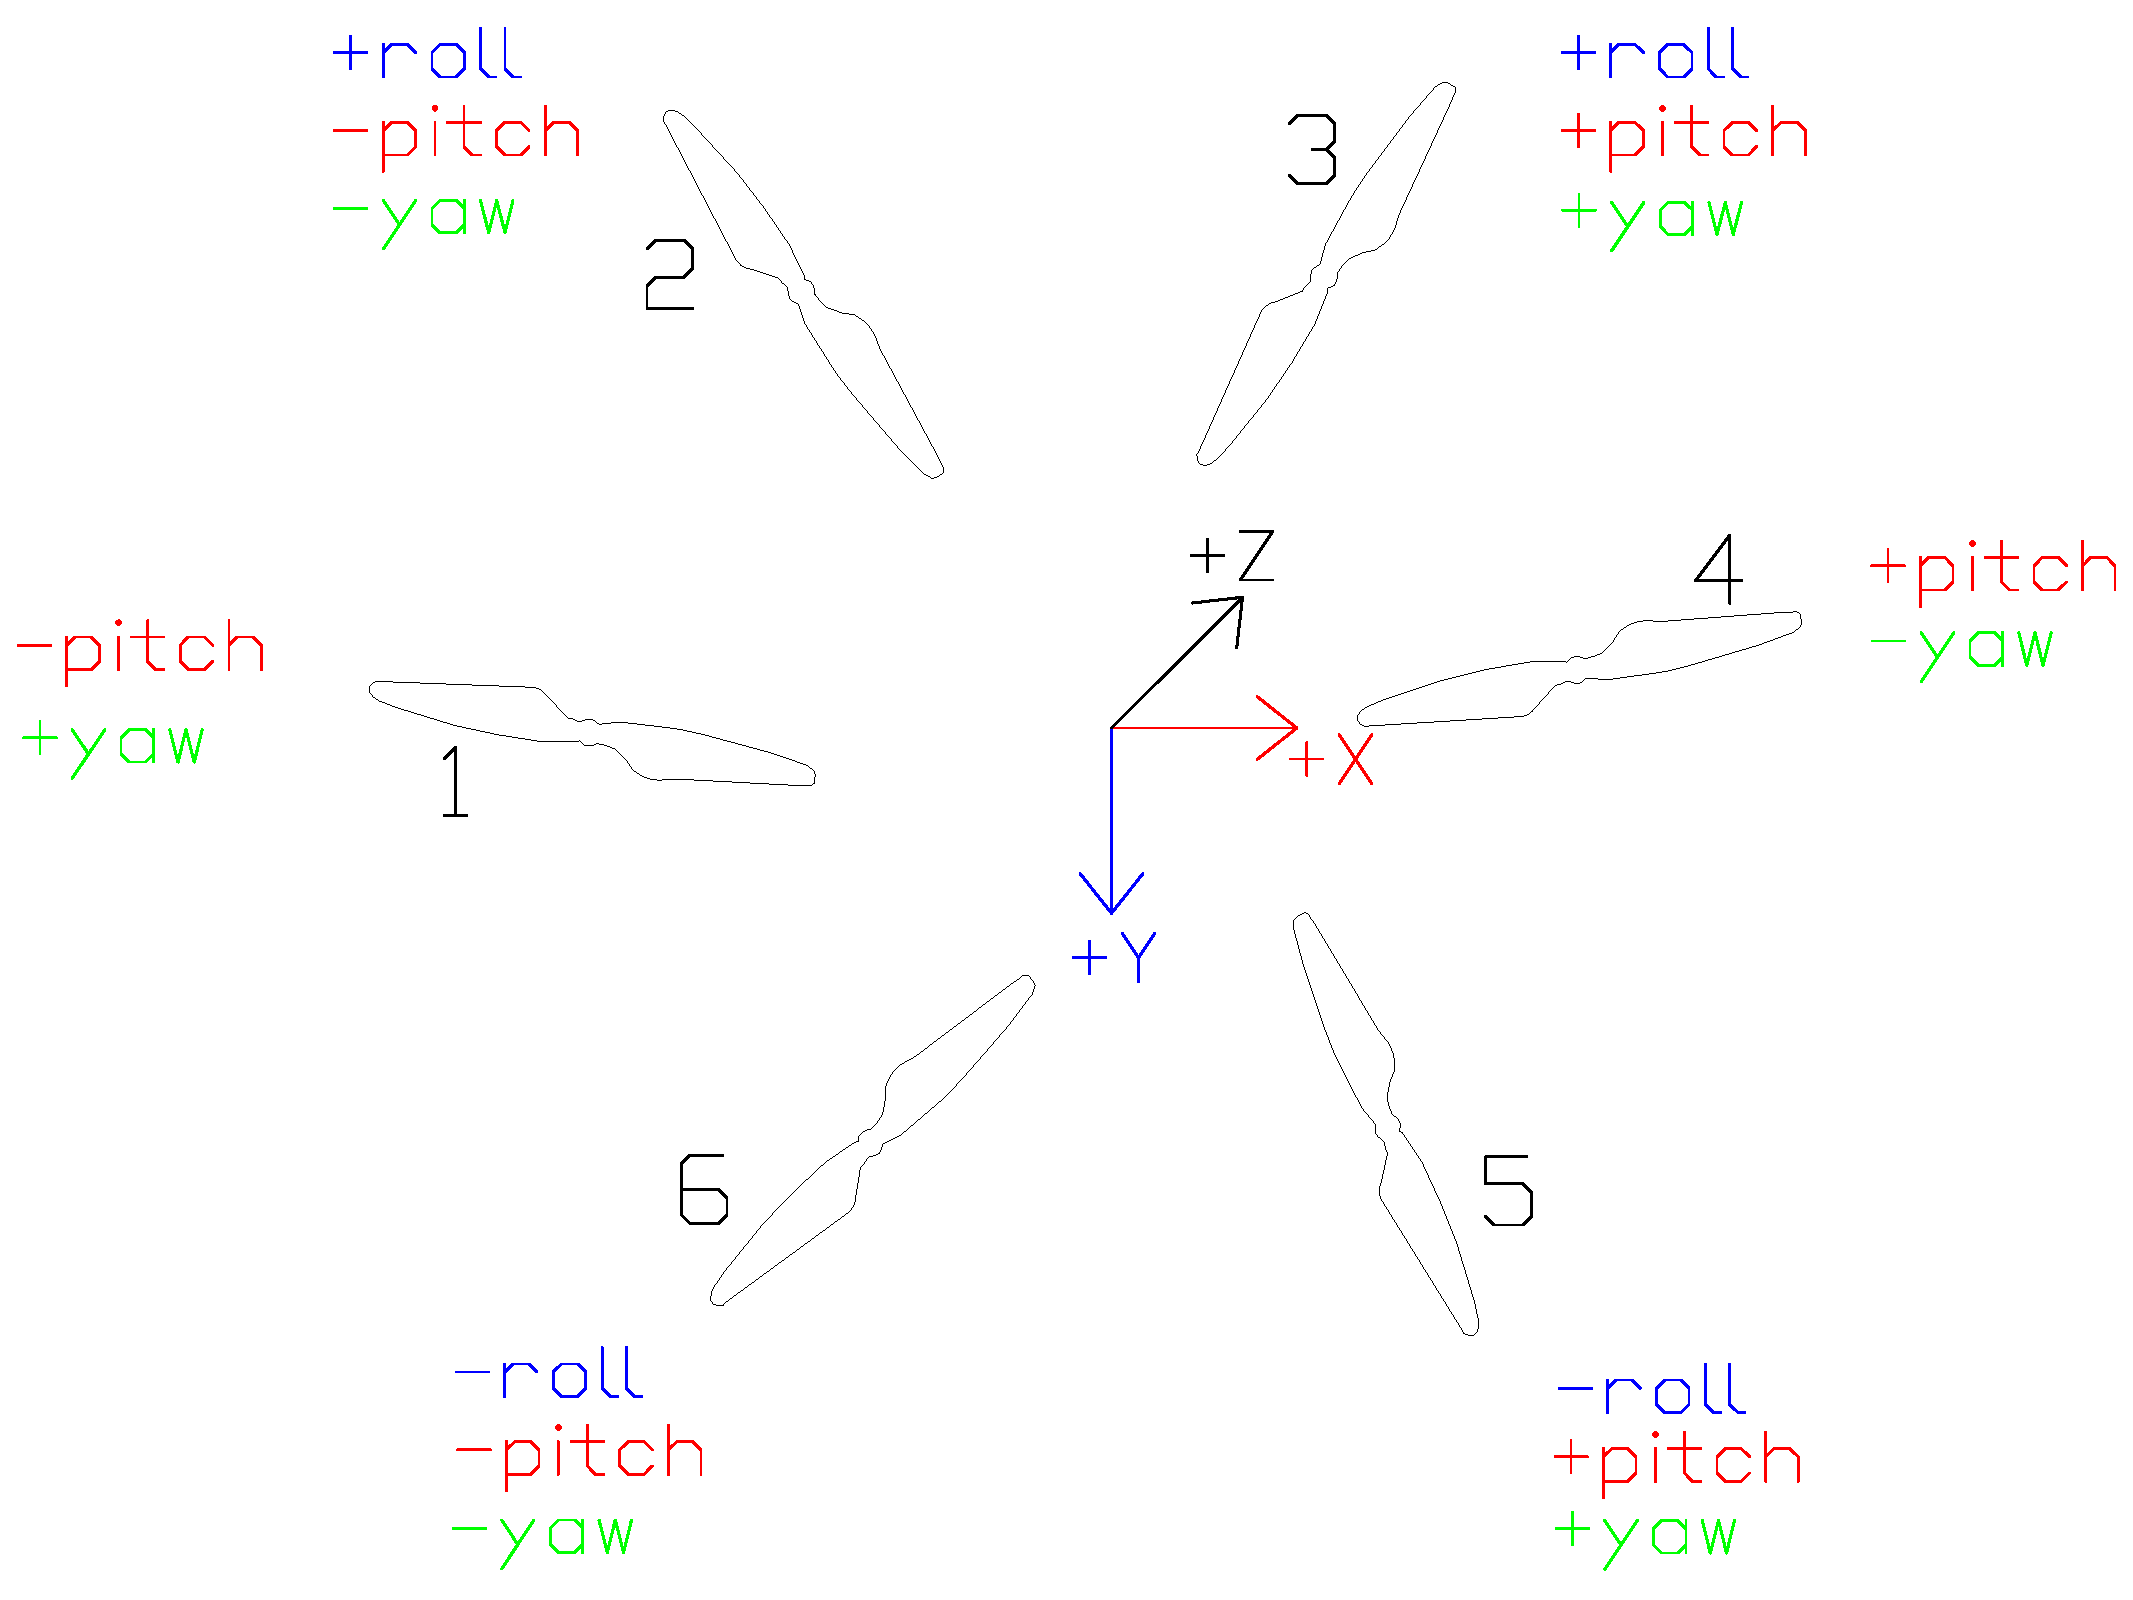
\includegraphics[width=9cm]{pictures/pid.pdf}
	\caption{Schéma ovládání dronu podle úhlu náklonu}
\end{figure}
\textbf{Pohybové rovnice}
\begin{eqnarray*} 
	motor1 & = & throttle - pidPitch           + pidYaw\\
	motor2 & = & throttle - pidPitch + pidRoll - pidYaw\\
	motor3 & = & throttle + pidPitch + pidRoll + pidYaw\\
	motor4 & = & throttle + pidPitch           - pidYaw\\
	motor5 & = & throttle + pidPitch - pidRoll + pidYaw\\
	motor6 & = & throttle - pidPitch - pidRoll - pidYaw\\
\end{eqnarray*} 

\begin{figure}[H]
	\centering
	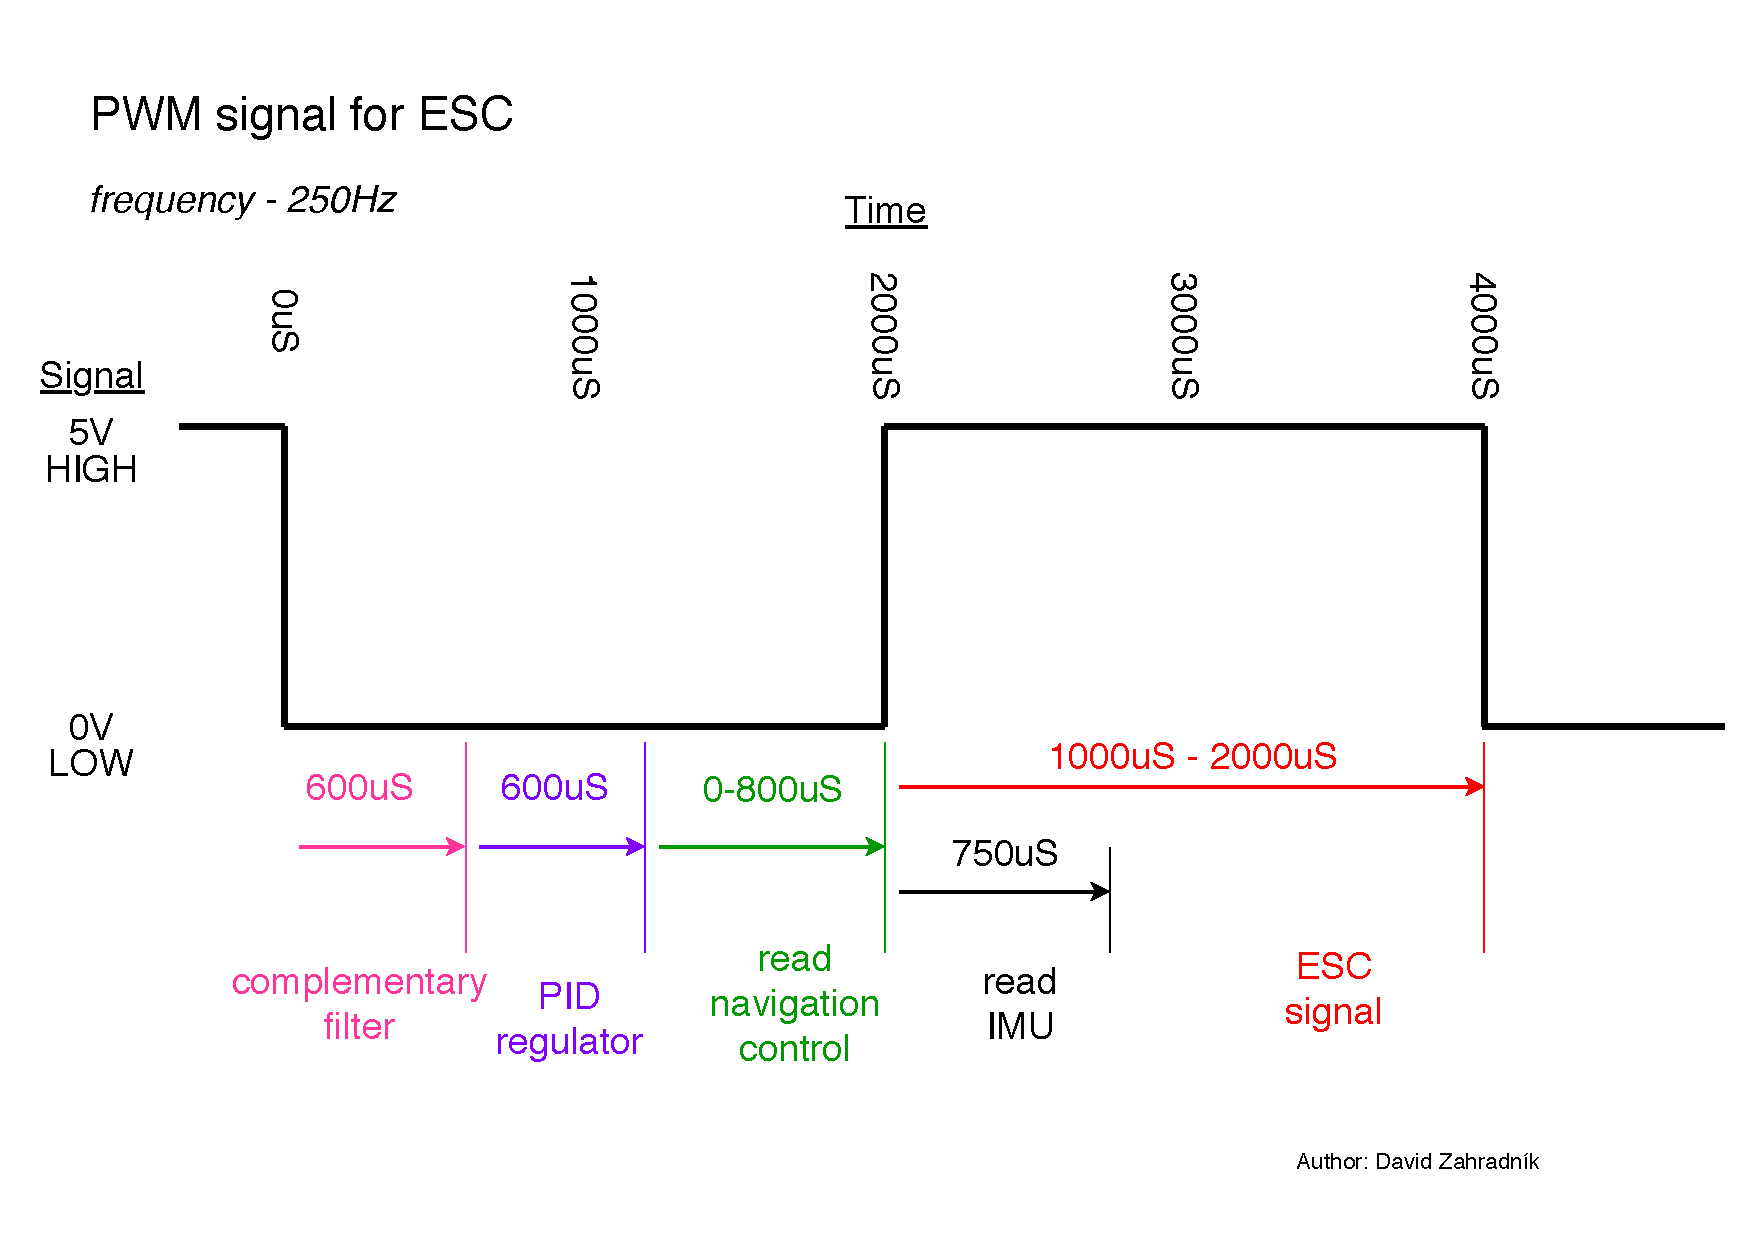
\includegraphics[width=16cm]{pictures/PWMDiagram.pdf}
	\caption{Diagram PWM signálu}
\end{figure}
\begin{figure}[H]
	\centering
	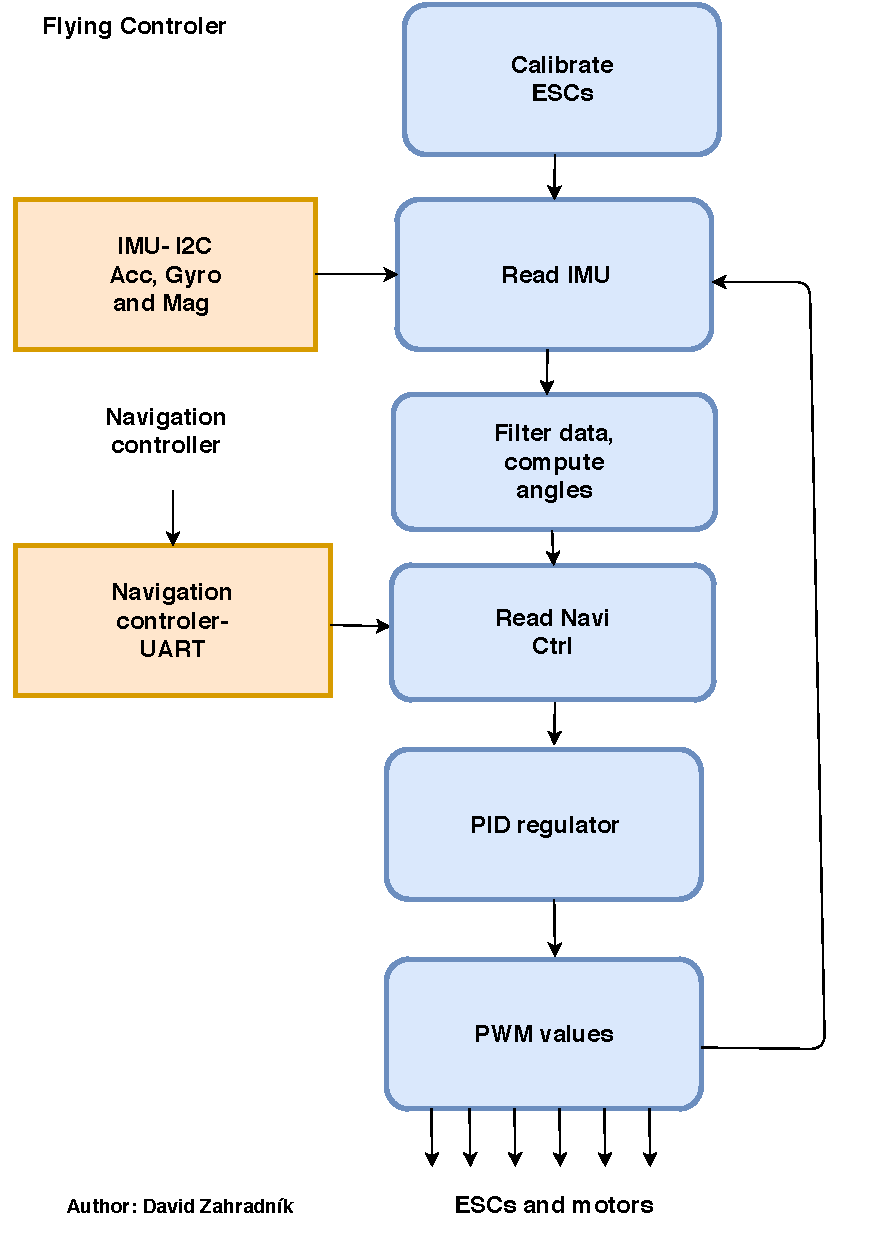
\includegraphics[width=12cm]{pictures/FlyingDiagram.pdf}
	\caption{Diagram algoritmu letového kontroléru}
\end{figure}
\begin{figure}[H]
	\centering
	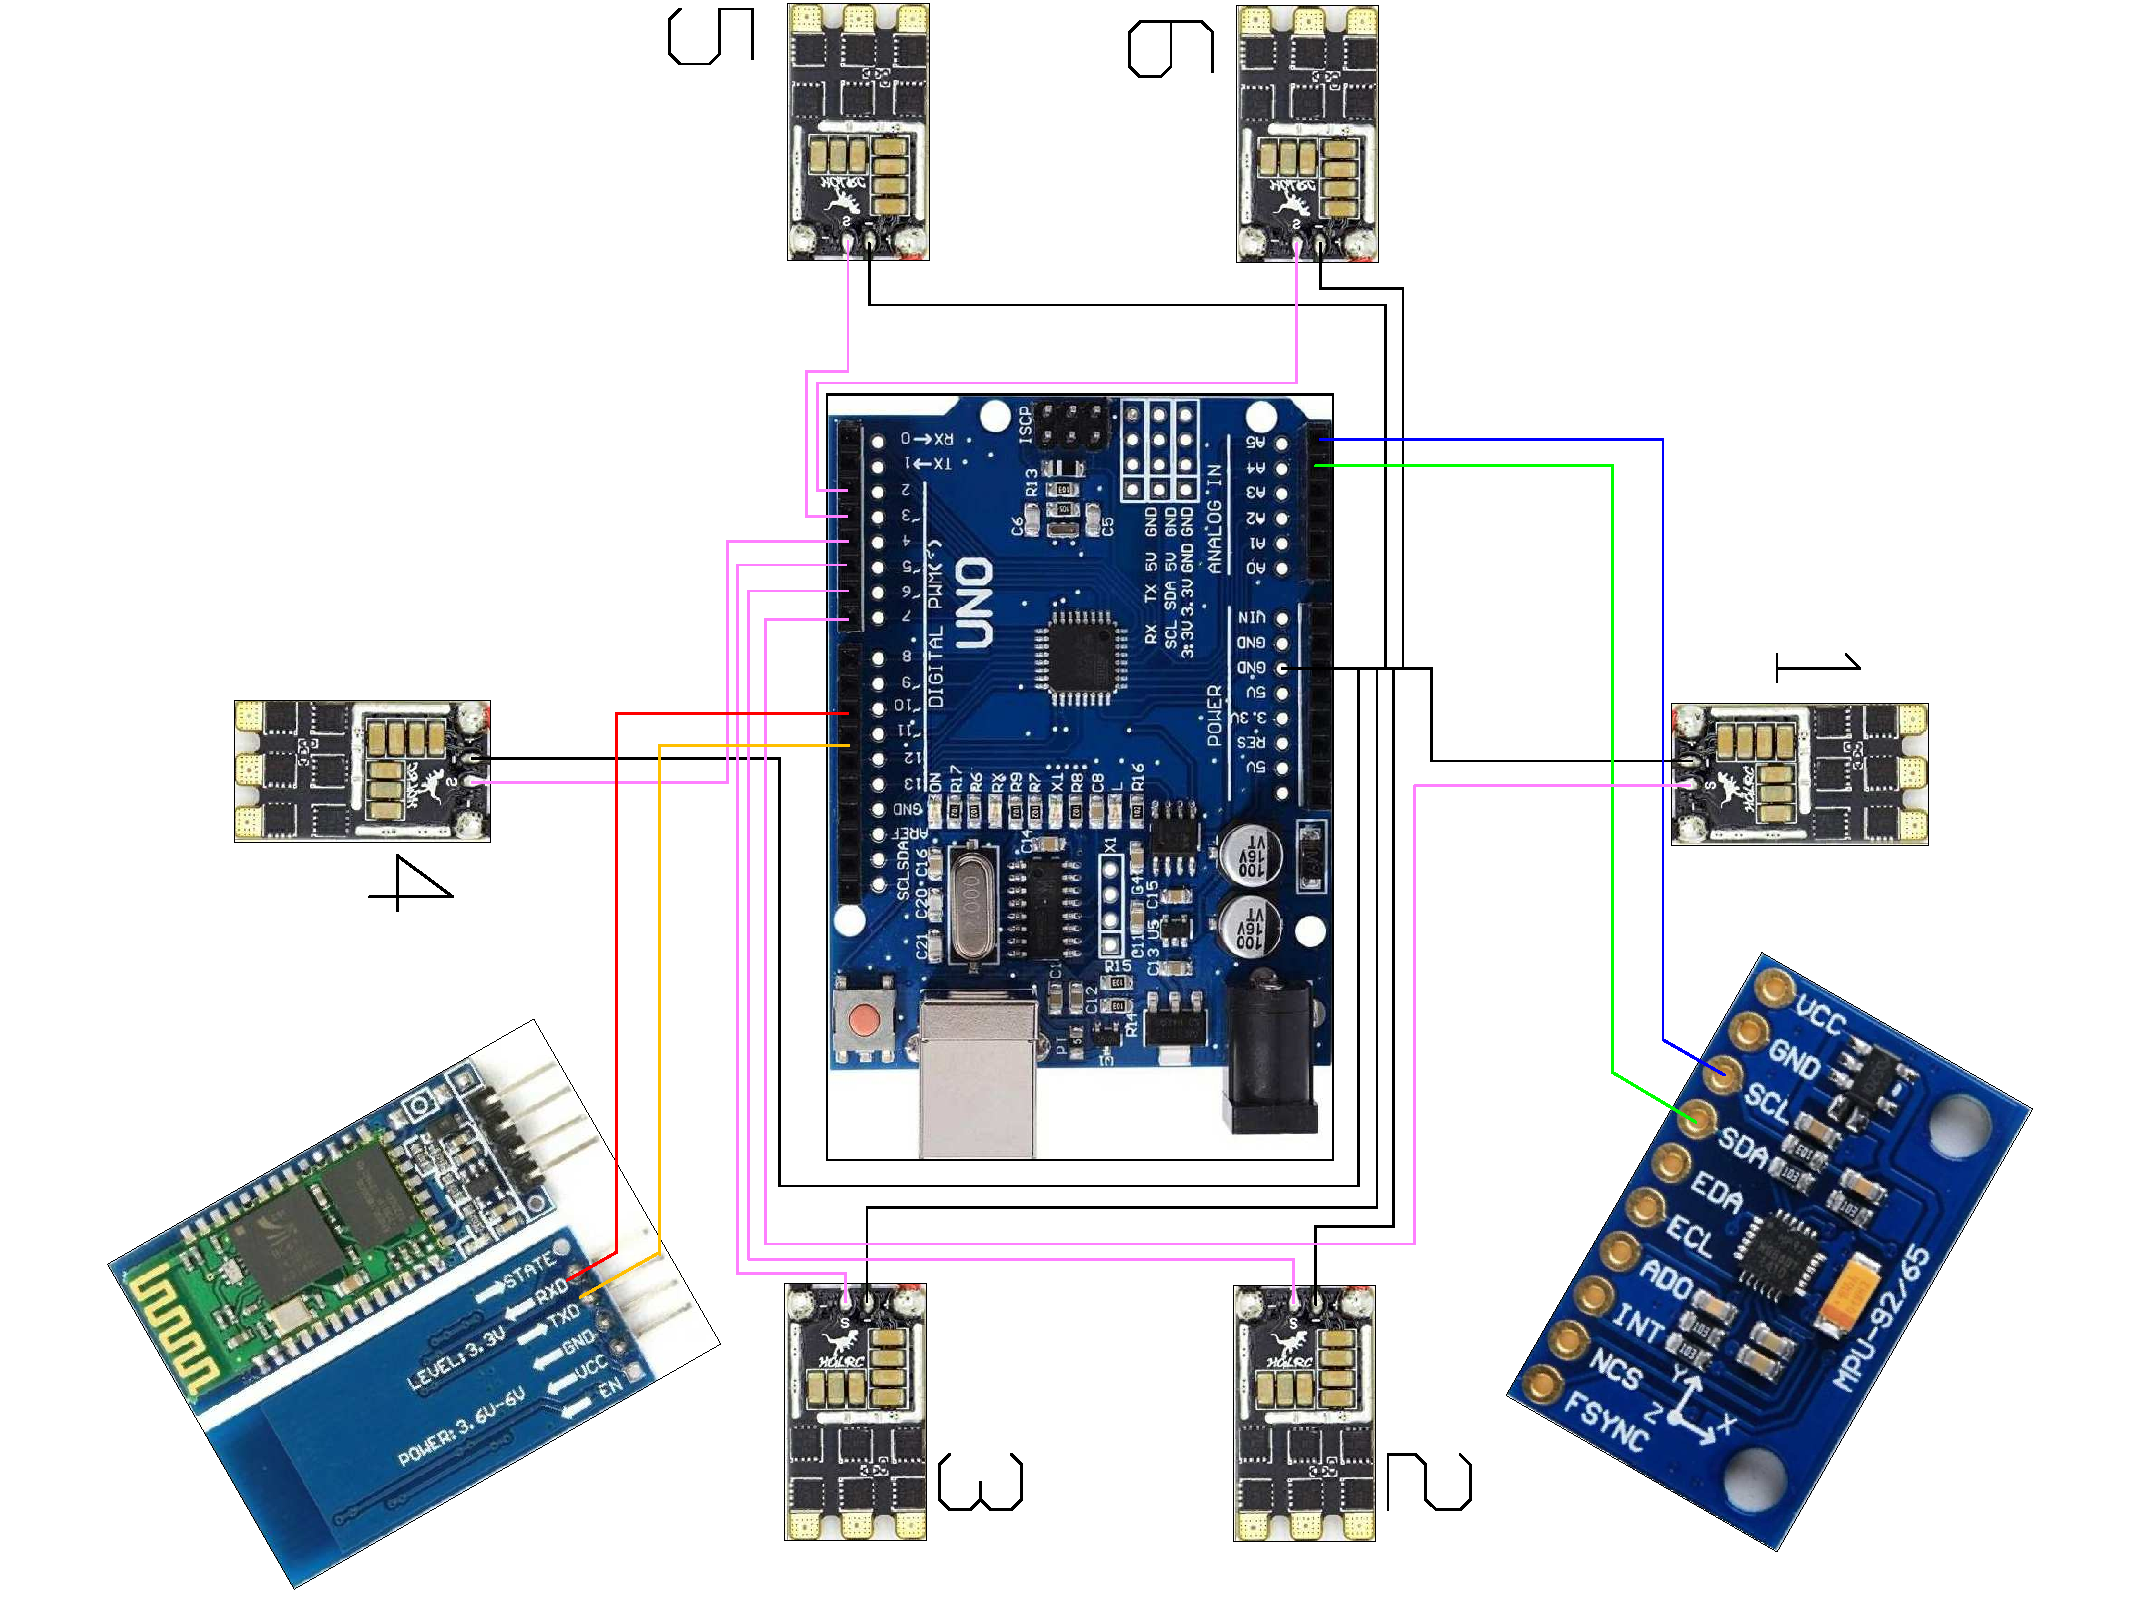
\includegraphics[width=12cm]{pictures/flyctrl.pdf}
	\caption{Schéma zapojení letového kontroléru}
\end{figure}

\section{Překážkový kontrolér} 
\textbf{Vstup:} 7x laserový modul\\
\textbf{Výstup:} Navigační kontrolér\\
Překážkový kontrolér upozorňuje navigační kontrolér o existenci cizího objektu v okolí dronu. Laserové moduly jsou nasměrovány do směrů pohybu podle úhlů pitch, roll a jeden laser je nasměrován po svislici pro přistávání. Lasery jsou nastaveny na kontinuální měření vzdáleností. Pokud se v blízkosti nachází cizí objekt, kontrolér pošle zprávu o překážce navigačnímu kontroléru a její poloze.\\

\begin{figure}[H]
	\centering
	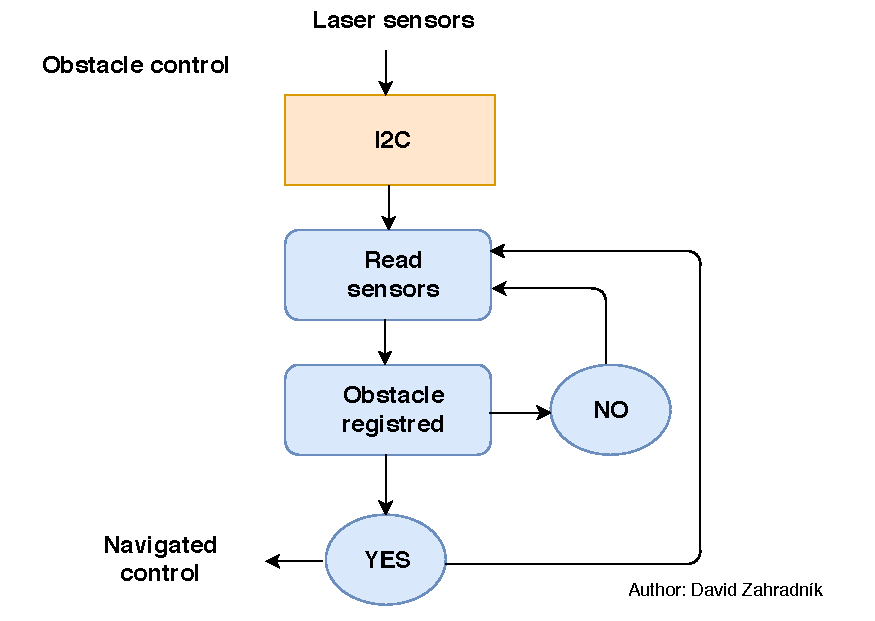
\includegraphics[width=12cm]{pictures/ObstacleDiagram.pdf}
	\caption{Diagram algoritmu překážkového kontroléru}
\end{figure}

\begin{figure}[H]
	\centering
	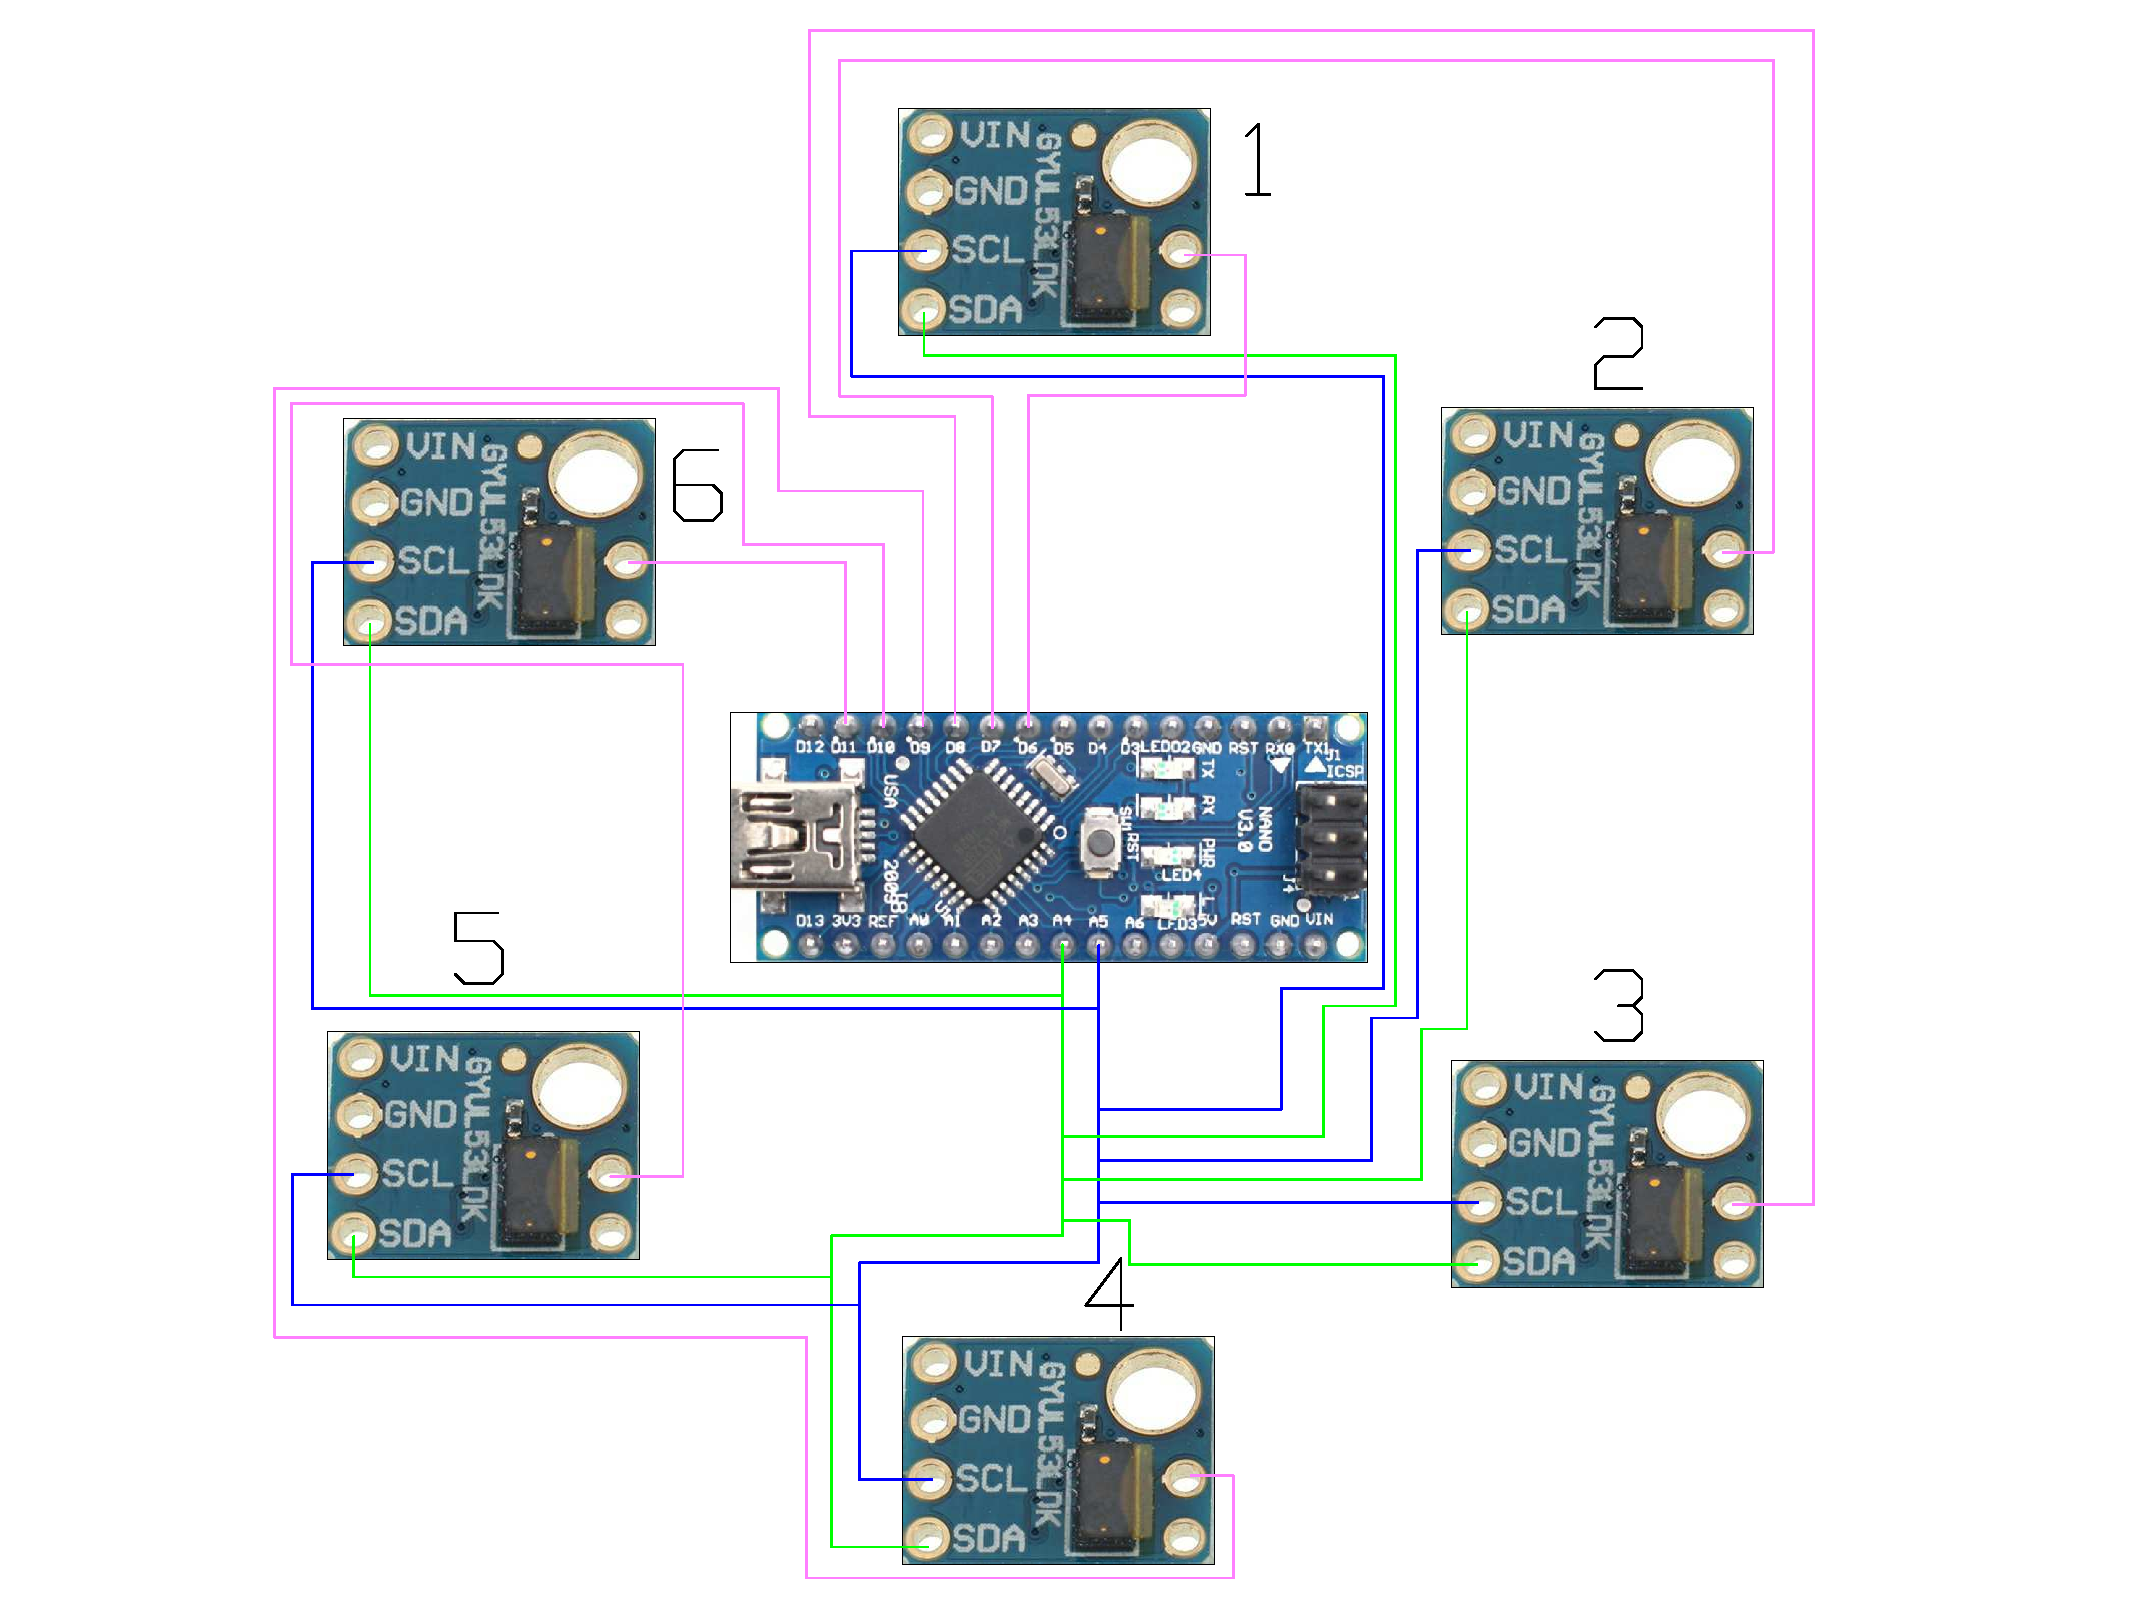
\includegraphics[width=10cm]{pictures/obstacle.pdf}
	\caption{Schéma zapojení Překážkového kontroléru}
\end{figure}

\begin{figure}[H]
	\centering
	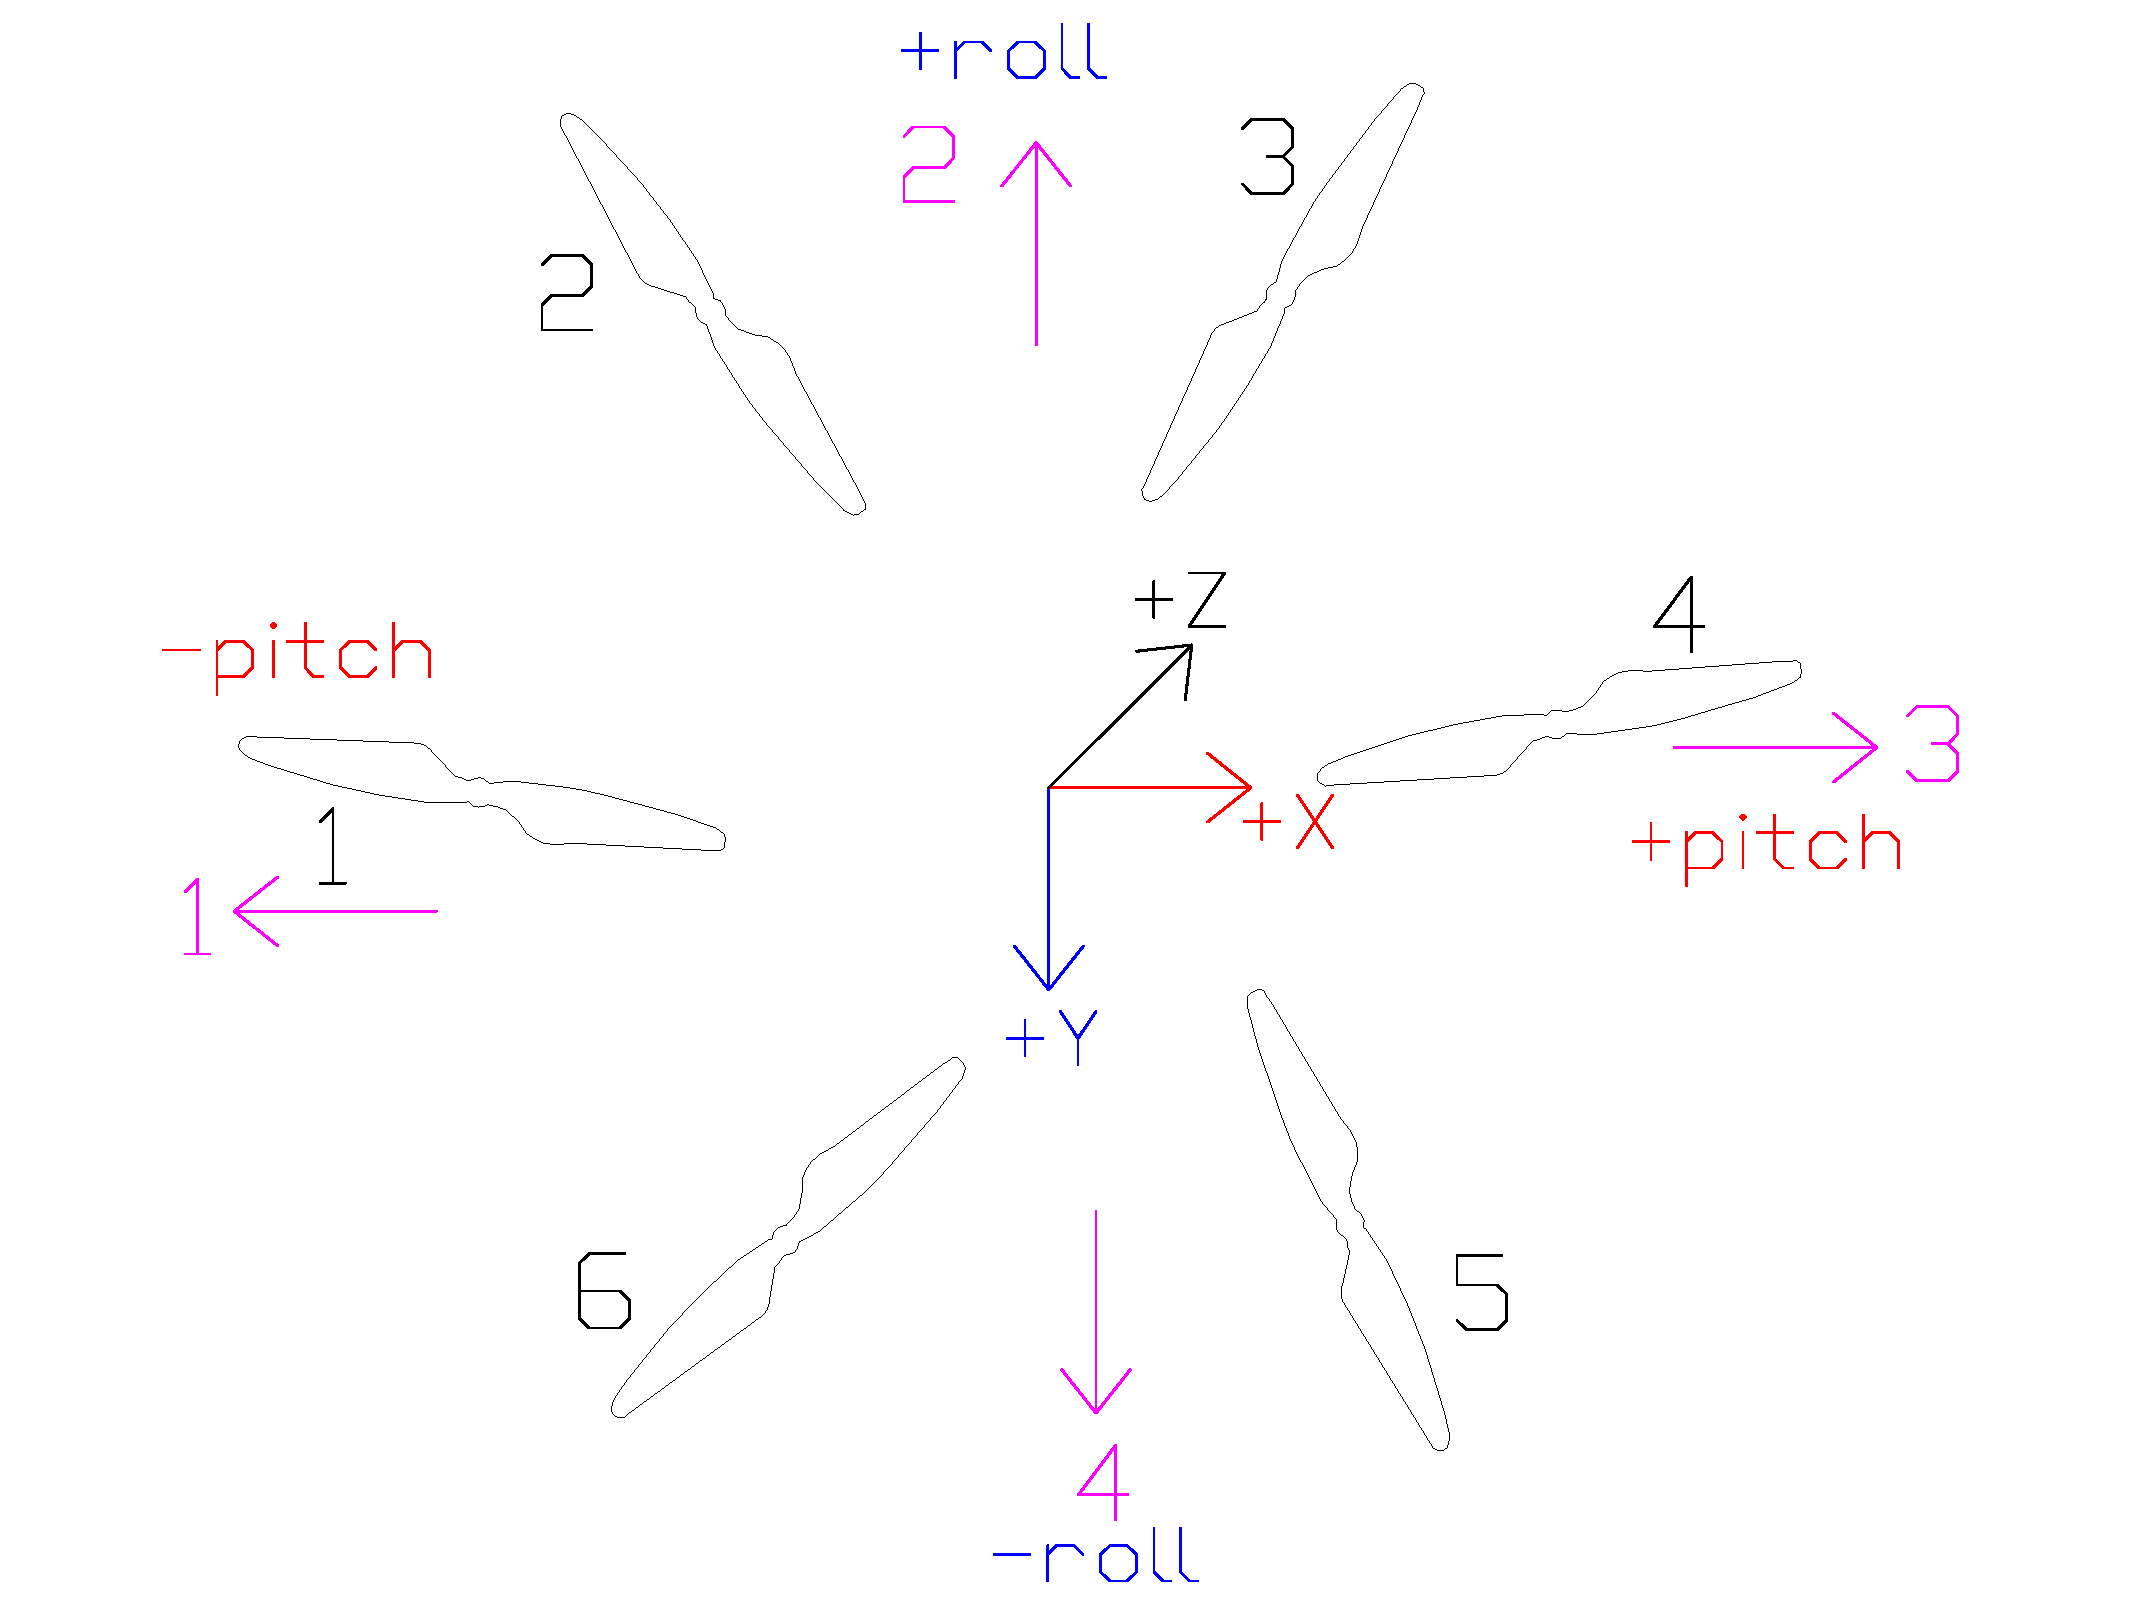
\includegraphics[width=10cm]{pictures/obstacle_teo.pdf}
	\caption{Schéma zpráv o překážce}
\end{figure}

\begin{table}[H]
	\centering
	\begin{tabular}{|l|l|l|}
		\hline
		\textbf{+/-} & \textbf{Úhel} & \textbf{Zpráva} \\ \hline
		+            & roll          & 2               \\ \hline
		-            & roll          & 4               \\ \hline
		-            & pitch         & 3               \\ \hline
		+            & pitch         & 1               \\ \hline
		& down          & 5               \\ \hline
	\end{tabular}
	\caption{Zpráva o překážce}
\end{table}

\section{Navigační kontrolér} 
\textbf{Vstup:} Rádio, Bluetooth, Barometr, GNSS, Překážkový kontrolér\\
\textbf{Výstup:} Letový kontrolér\\
Navigační kontrolér složí ke komunikaci s ovládacím zařízením, sběru dat z gnss, barometru a překážkového kontroléru.\\
Po zapnutí bude kontrolér čekat na zprávu ze smartphonu. Podle typu příchozích dat kontrolér nastaví autonomní nebo manuální řízení.\\
Používá-li uživatel manuální ovládání, navigační kontrolér pouze ověří zda existuje překážka, pokud existuje, zámezí srážce. Neexistuje-li překážka kontrolér pošle data letovému kontroléru.\\
Při autonomním ovládání kontrolér porovná data z GNSS aparatury a zadané souřadnice. Pokud souřadnice nejsou totožné, vypočte se směr a vzdálenost z polohy dronu a zadaných souřadnic. Provede se shodnostní transformace ze souřadnicového systému GNSS aparatury do souřadnicového systému dronu. Vstupní data pro PID regulátor budou souřadnicové rozdíly v souřadnicovém systému dronu a výstupní data budou úhly pitch a roll.\\
Při držení určité nadmořské výšky se zvovu použije PID regulátor. Vstupním datem bude nadmořská výška z GNSS aparatury nebo z barometru, výstupem bude výkon motoru, který bude konstatní pro všechny motory.\\
Bude definována funkce návrat, při které se dron vrátí na startovní místo. Pozice startovního místa bude změřena GNSS aparaturou automaticky před startem dronu.\\

\begin{figure}[H]
	\centering
	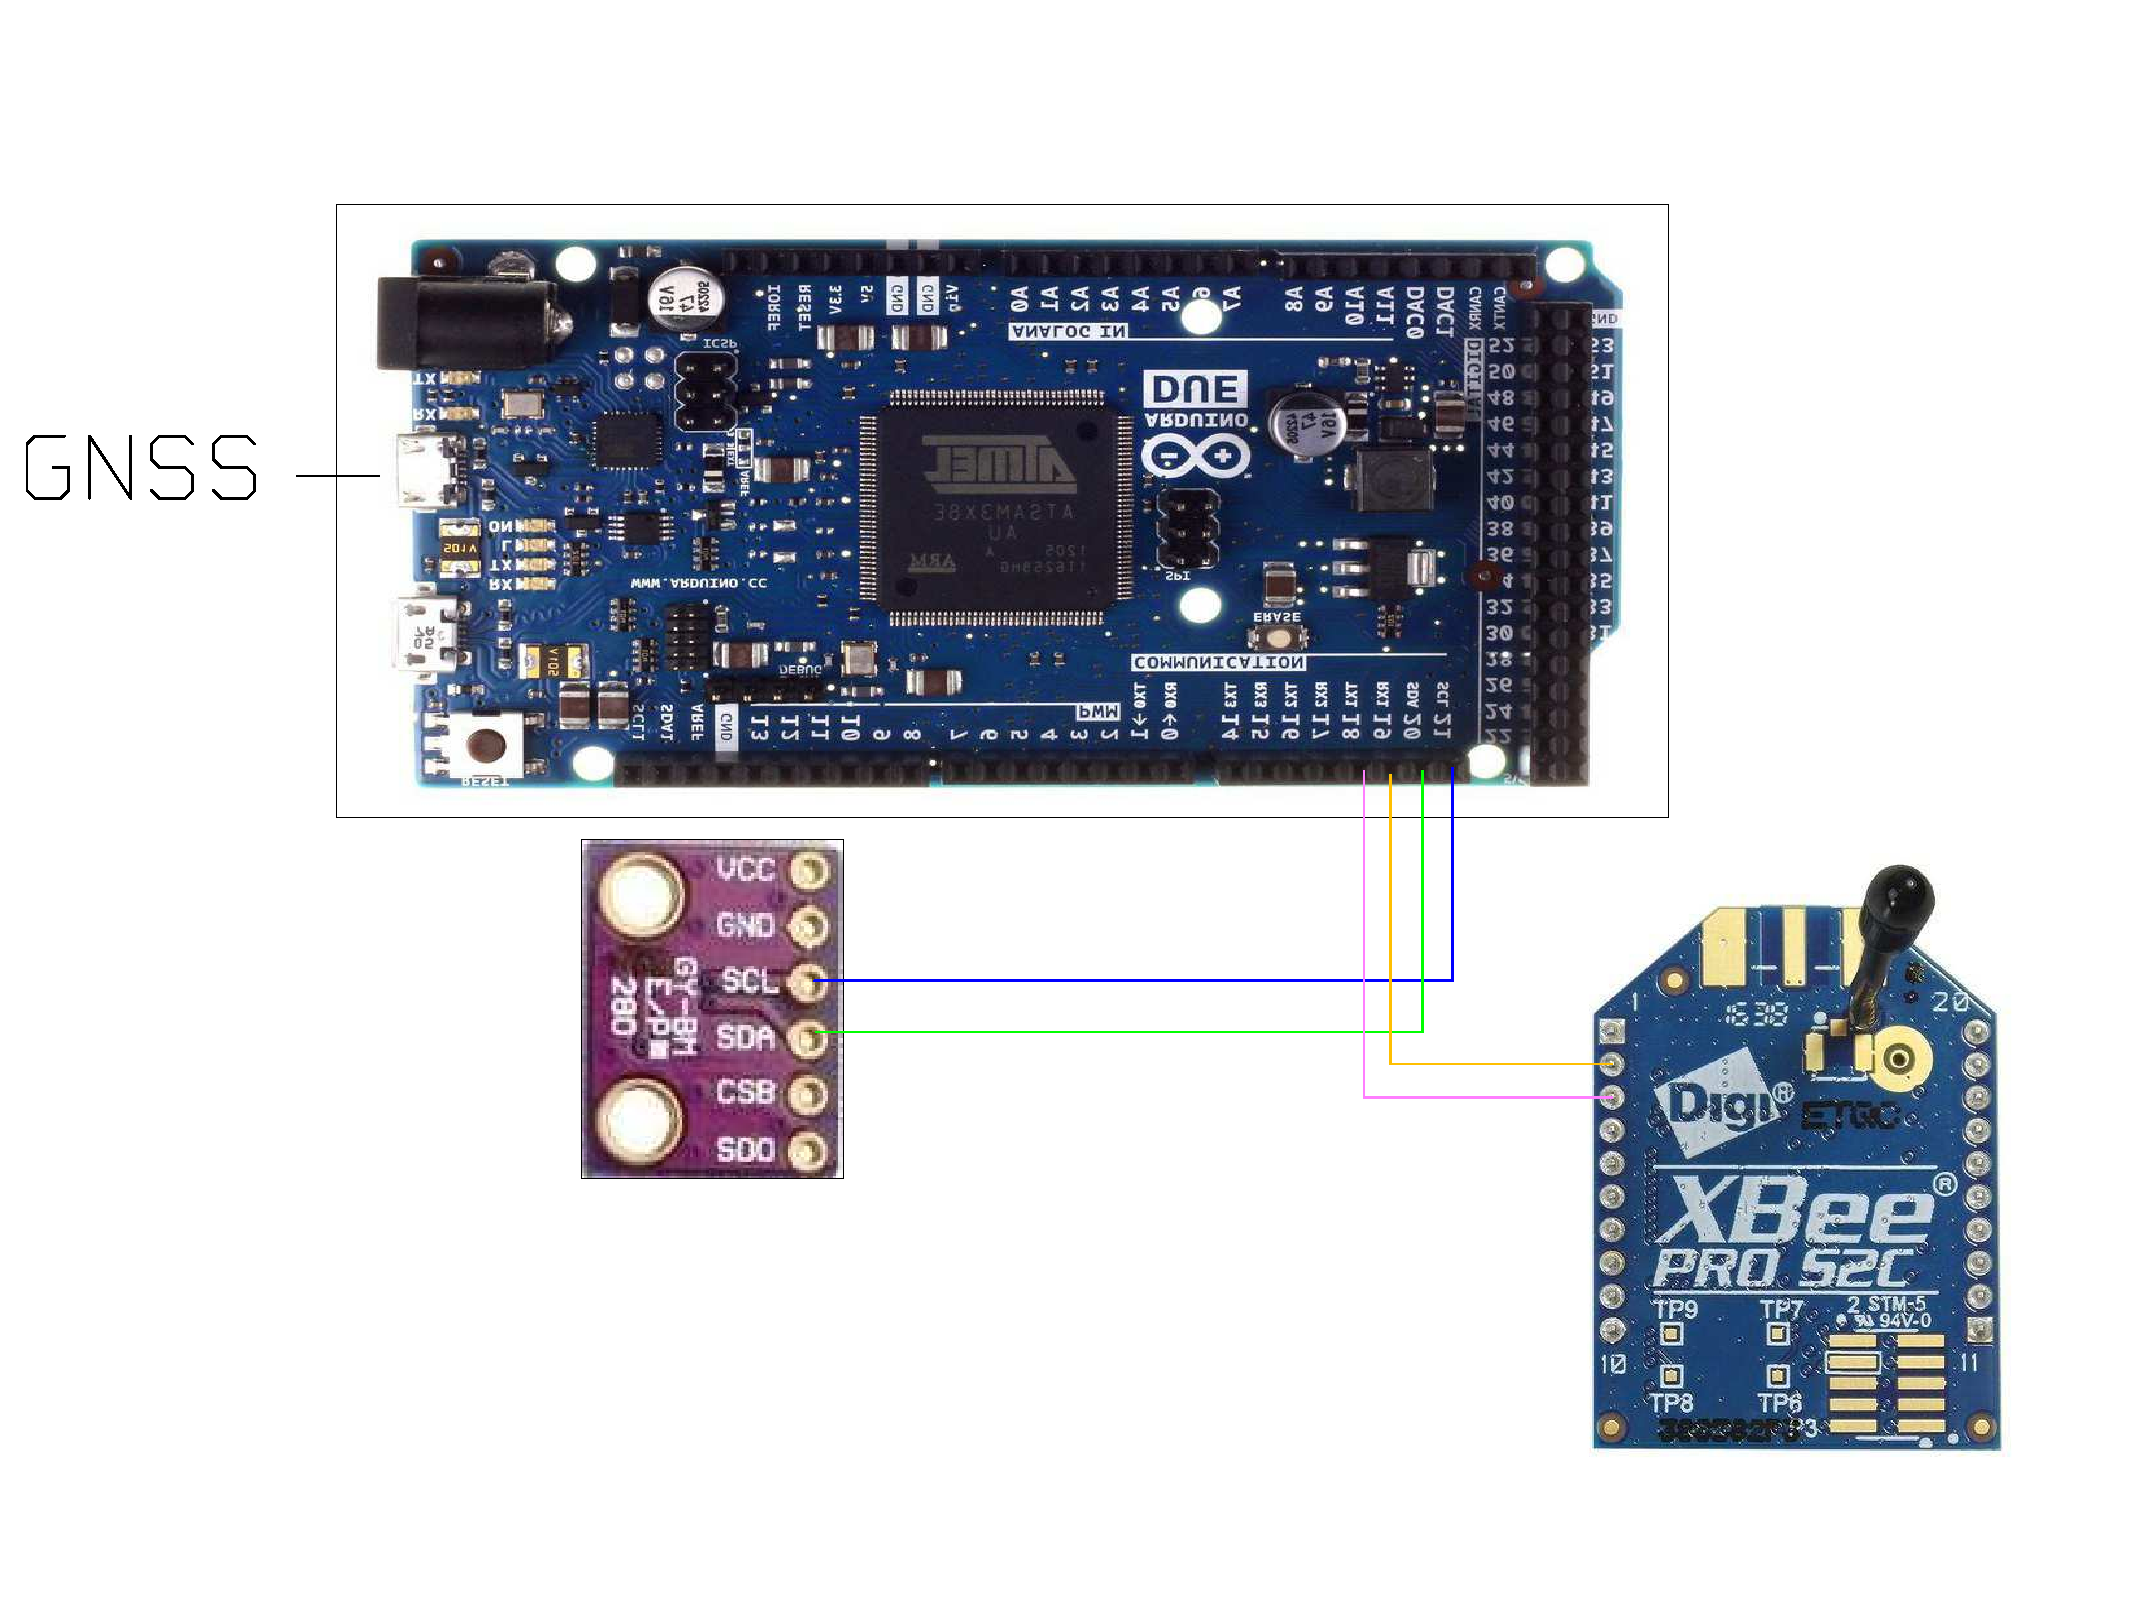
\includegraphics[width=10cm]{pictures/navictrl.pdf}
	\caption{Schéma zapojení Navigačního kontroléru}
\end{figure}
\begin{figure}[H]
	\centering
	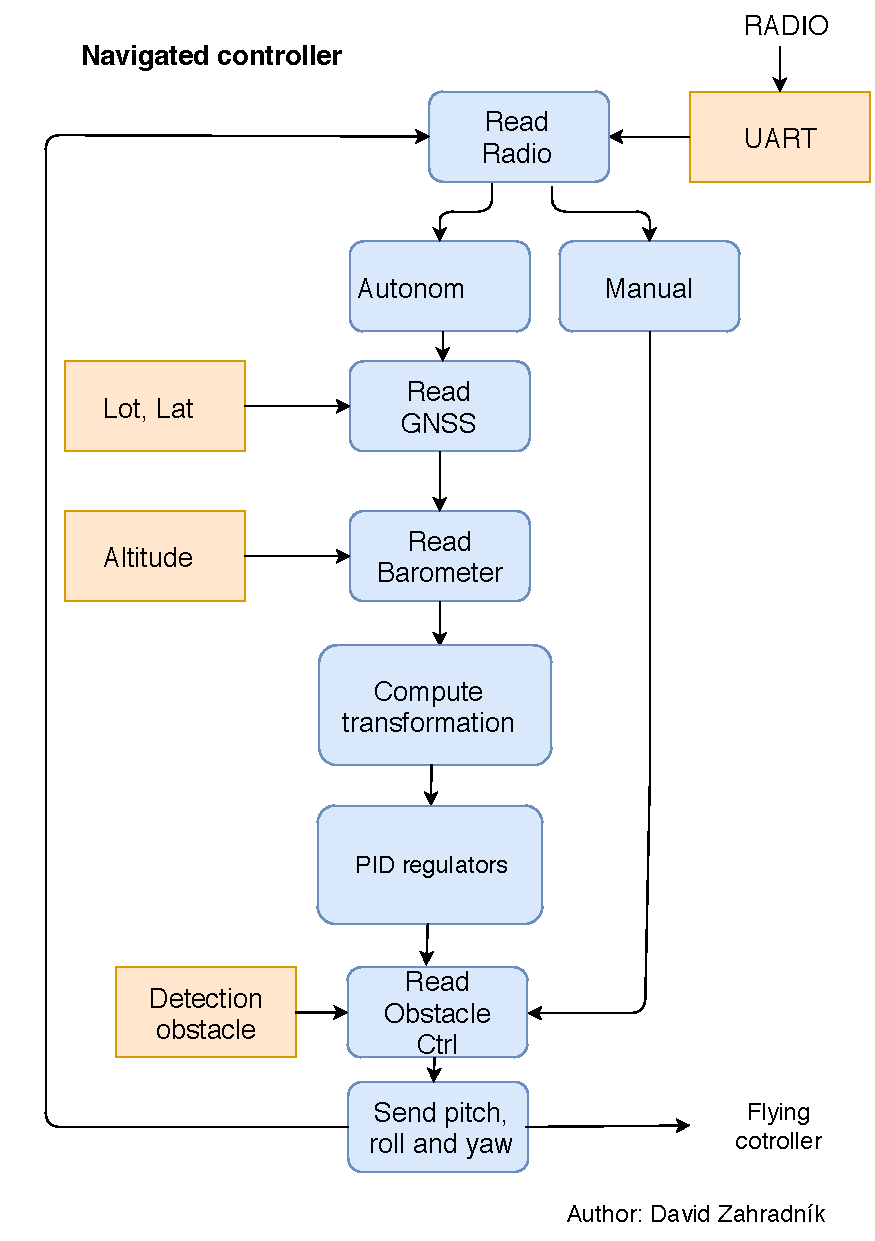
\includegraphics[width=14cm]{pictures/NaviDiagram.pdf}
	\caption{Diagram navigačního kontroléru}
\end{figure}


\section{Finální sestavení}
Z důvodů nízkého výpočetního výkonu platfromy Arduino je komplení ovládání sestaveno ze tří platforem Arduino. Letový kontrolér ovládá jednotlivé motory, překážkový kontrolér detekuje případné překážky a navigační kontrolér komunikuje s ovladačem a řídí let.\\
Distribuční deska s regulátory otáček jsou umístěny ve spodní části dronu pod baterii. Byl zjištěn negativní vliv magnetického pole regulátorů pro ovládací prvky. Magnetické pole bylo tak silné, že ovládací prvky byly neovladatelné. Ovládací prvky jsou umístěné na vrchní části dronu. Barometr a GNSS aparatura jsou vyvýšené nad vrtulemi, aby tlak vzduchu neovlivňoval jejich funkčnost.\\
Dron je ovládán smartphonem přes uzlové zařízení. Uzlové zařízení se skládá z bluetooth a radiového modulu. Tok dat probíhá ze smartphonu přes bluetooth do uzlového zařízení a ze zařízení do navigačního kontroléru přes radiový signál.\\
Kamera posílá data smartphonu nezávisle na ovládání dronu. Kamera obsahuje vlastní radiový vysílač, který vysílá data přijímači připojeného k smartphonu skrze miniUSB. Pro správnou funkci kamery musí smartphone podporovat funkci OTG.\\
Při připevnění IMU jednotky kovovými šrouby na konstrukci dronu, byl zjištěn ne\-gativní vliv kovu na data z IMU, proto všechny řídící komponenty jsou připevněny k nepájivému poli.\\
\begin{figure}[h]
	\centering
	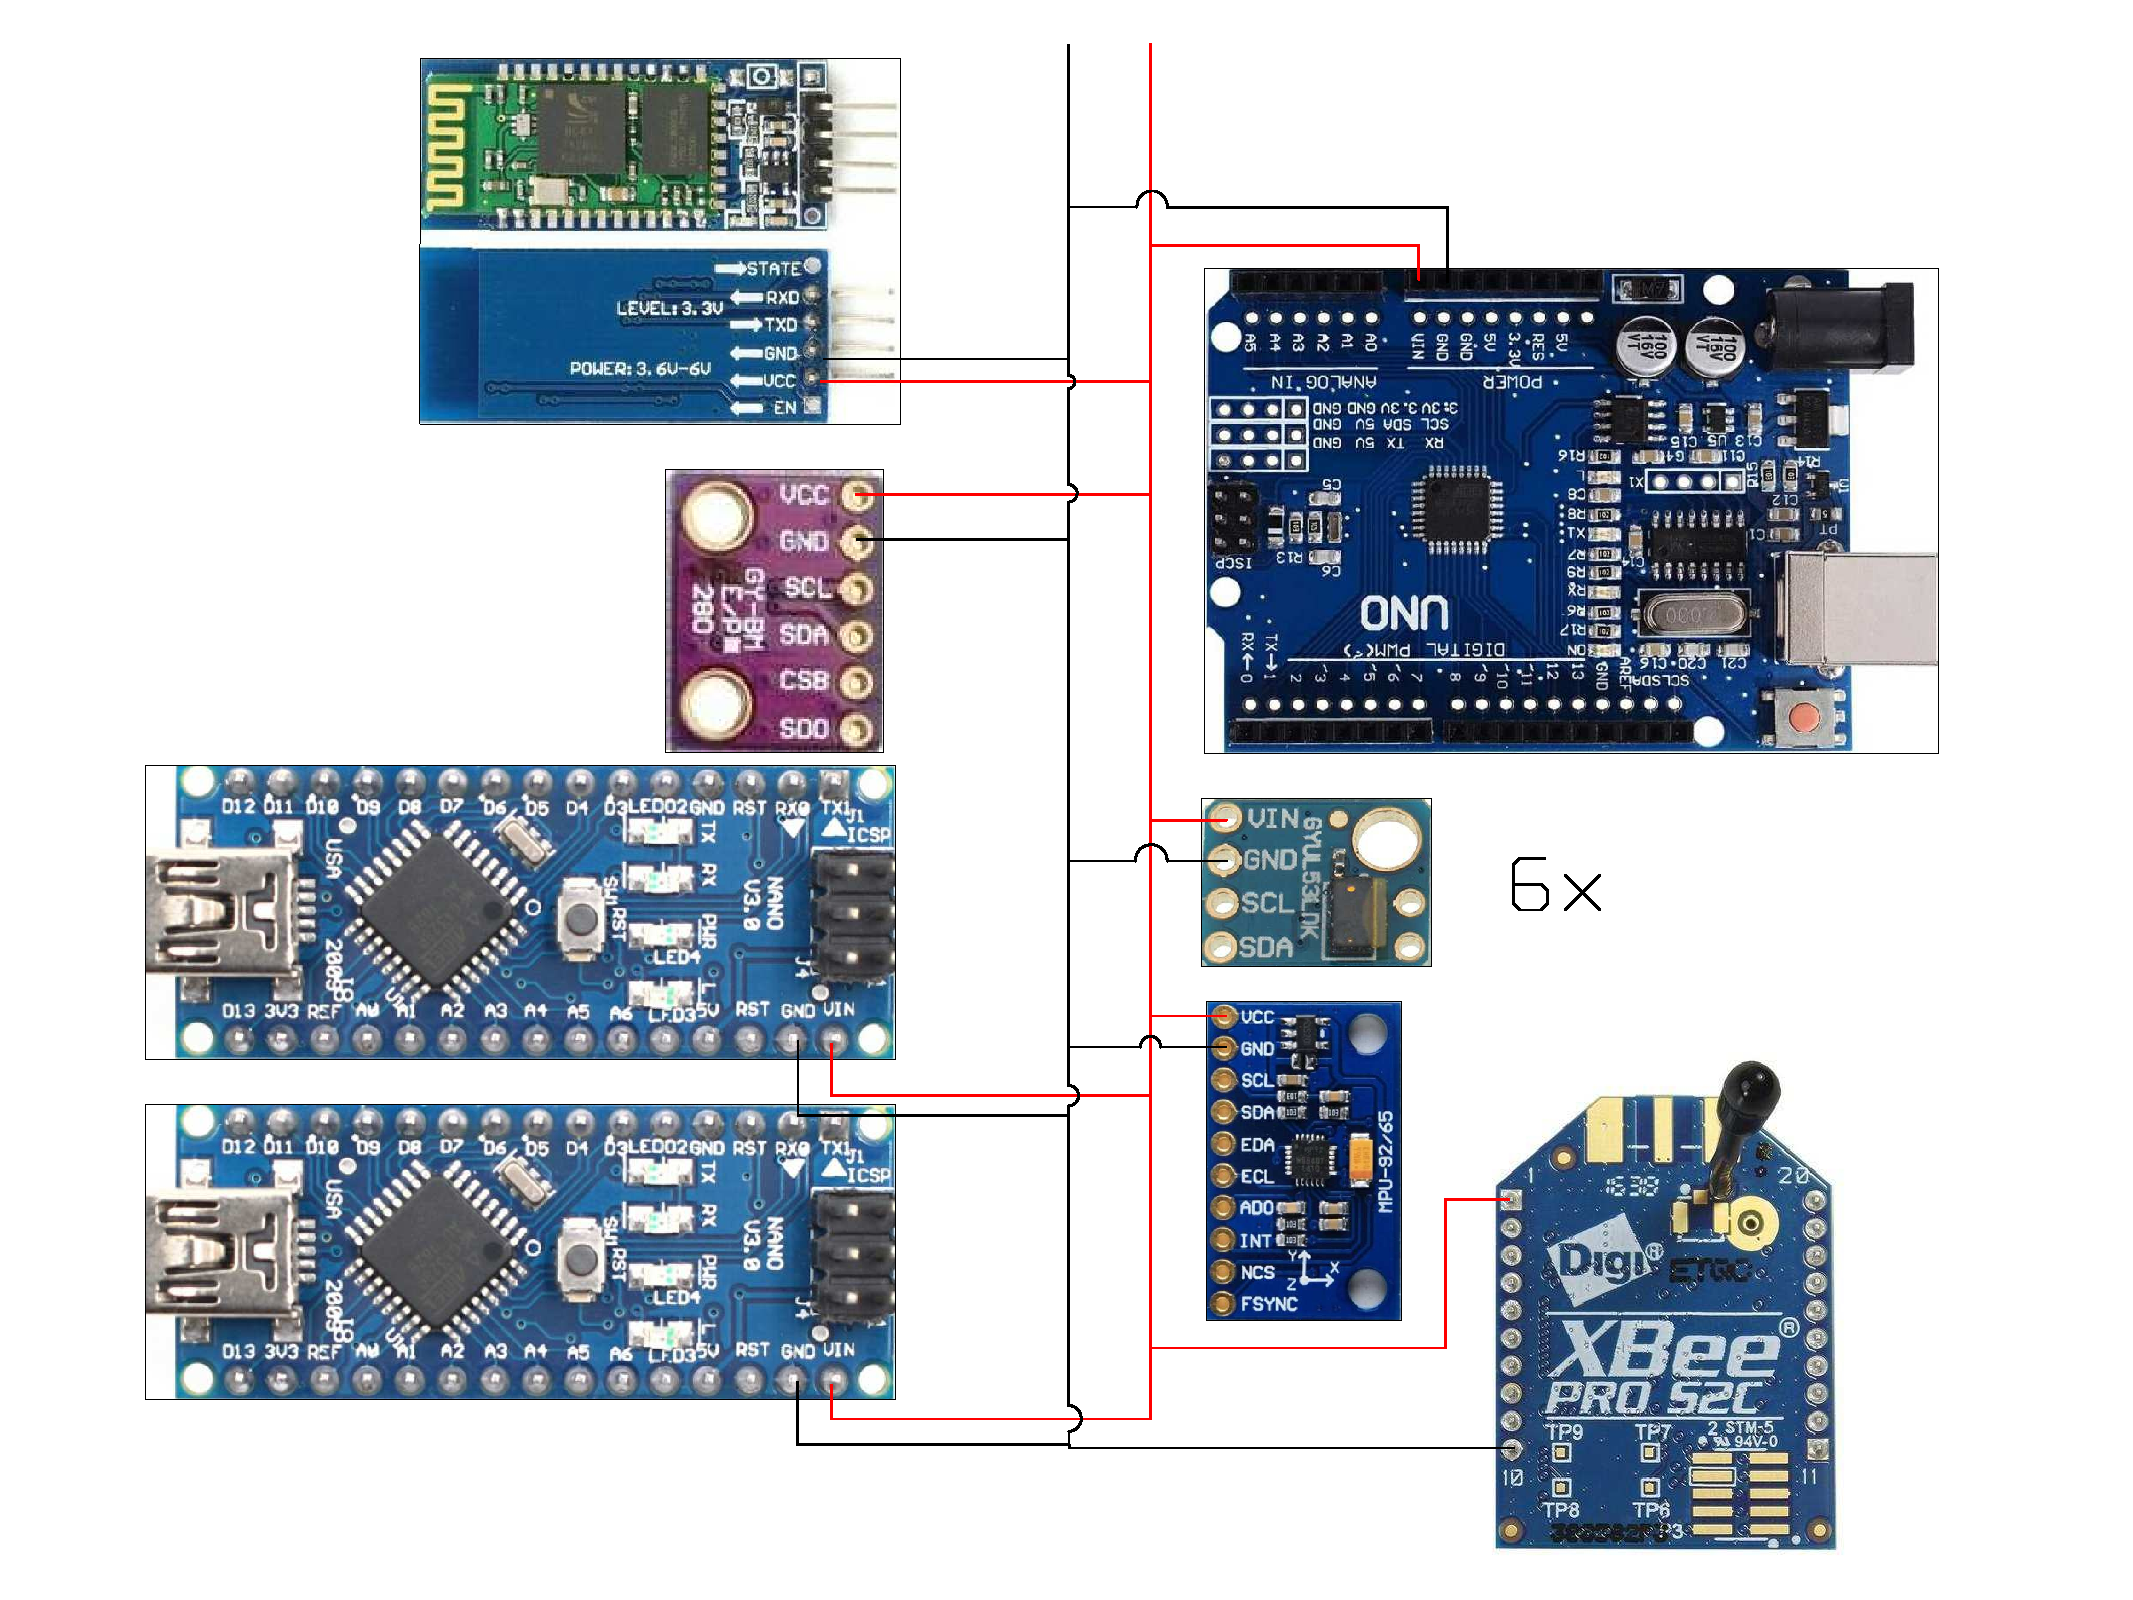
\includegraphics[width=10cm]{pictures/pdb_ardu.pdf}
	\caption{Schéma zapojení napájení Arduina a modulů}
\end{figure}
\begin{figure}[H]
	\centering
	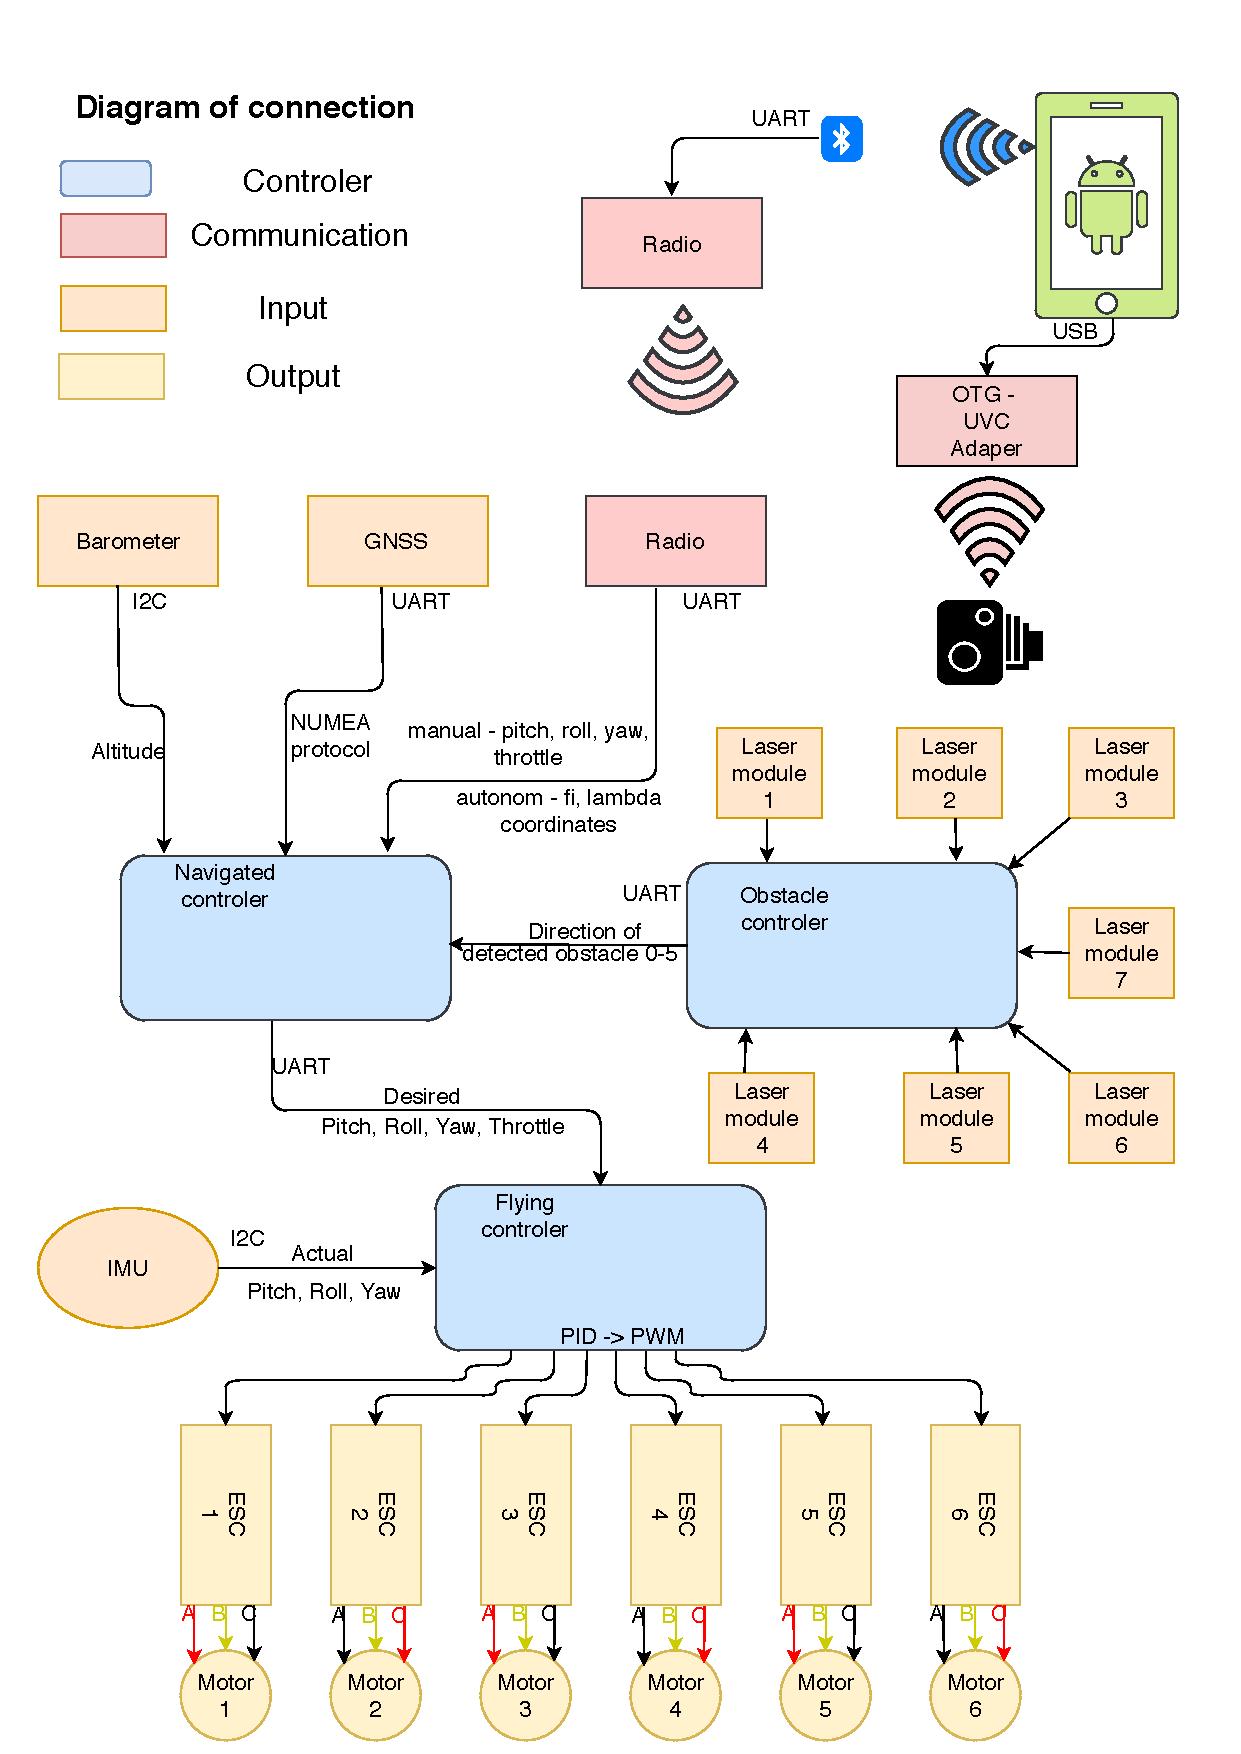
\includegraphics[width=15cm]{pictures/DroneDiagram.pdf}
	\caption{Diagram komponent}
\end{figure}
\begin{figure}[h]
	\centering
	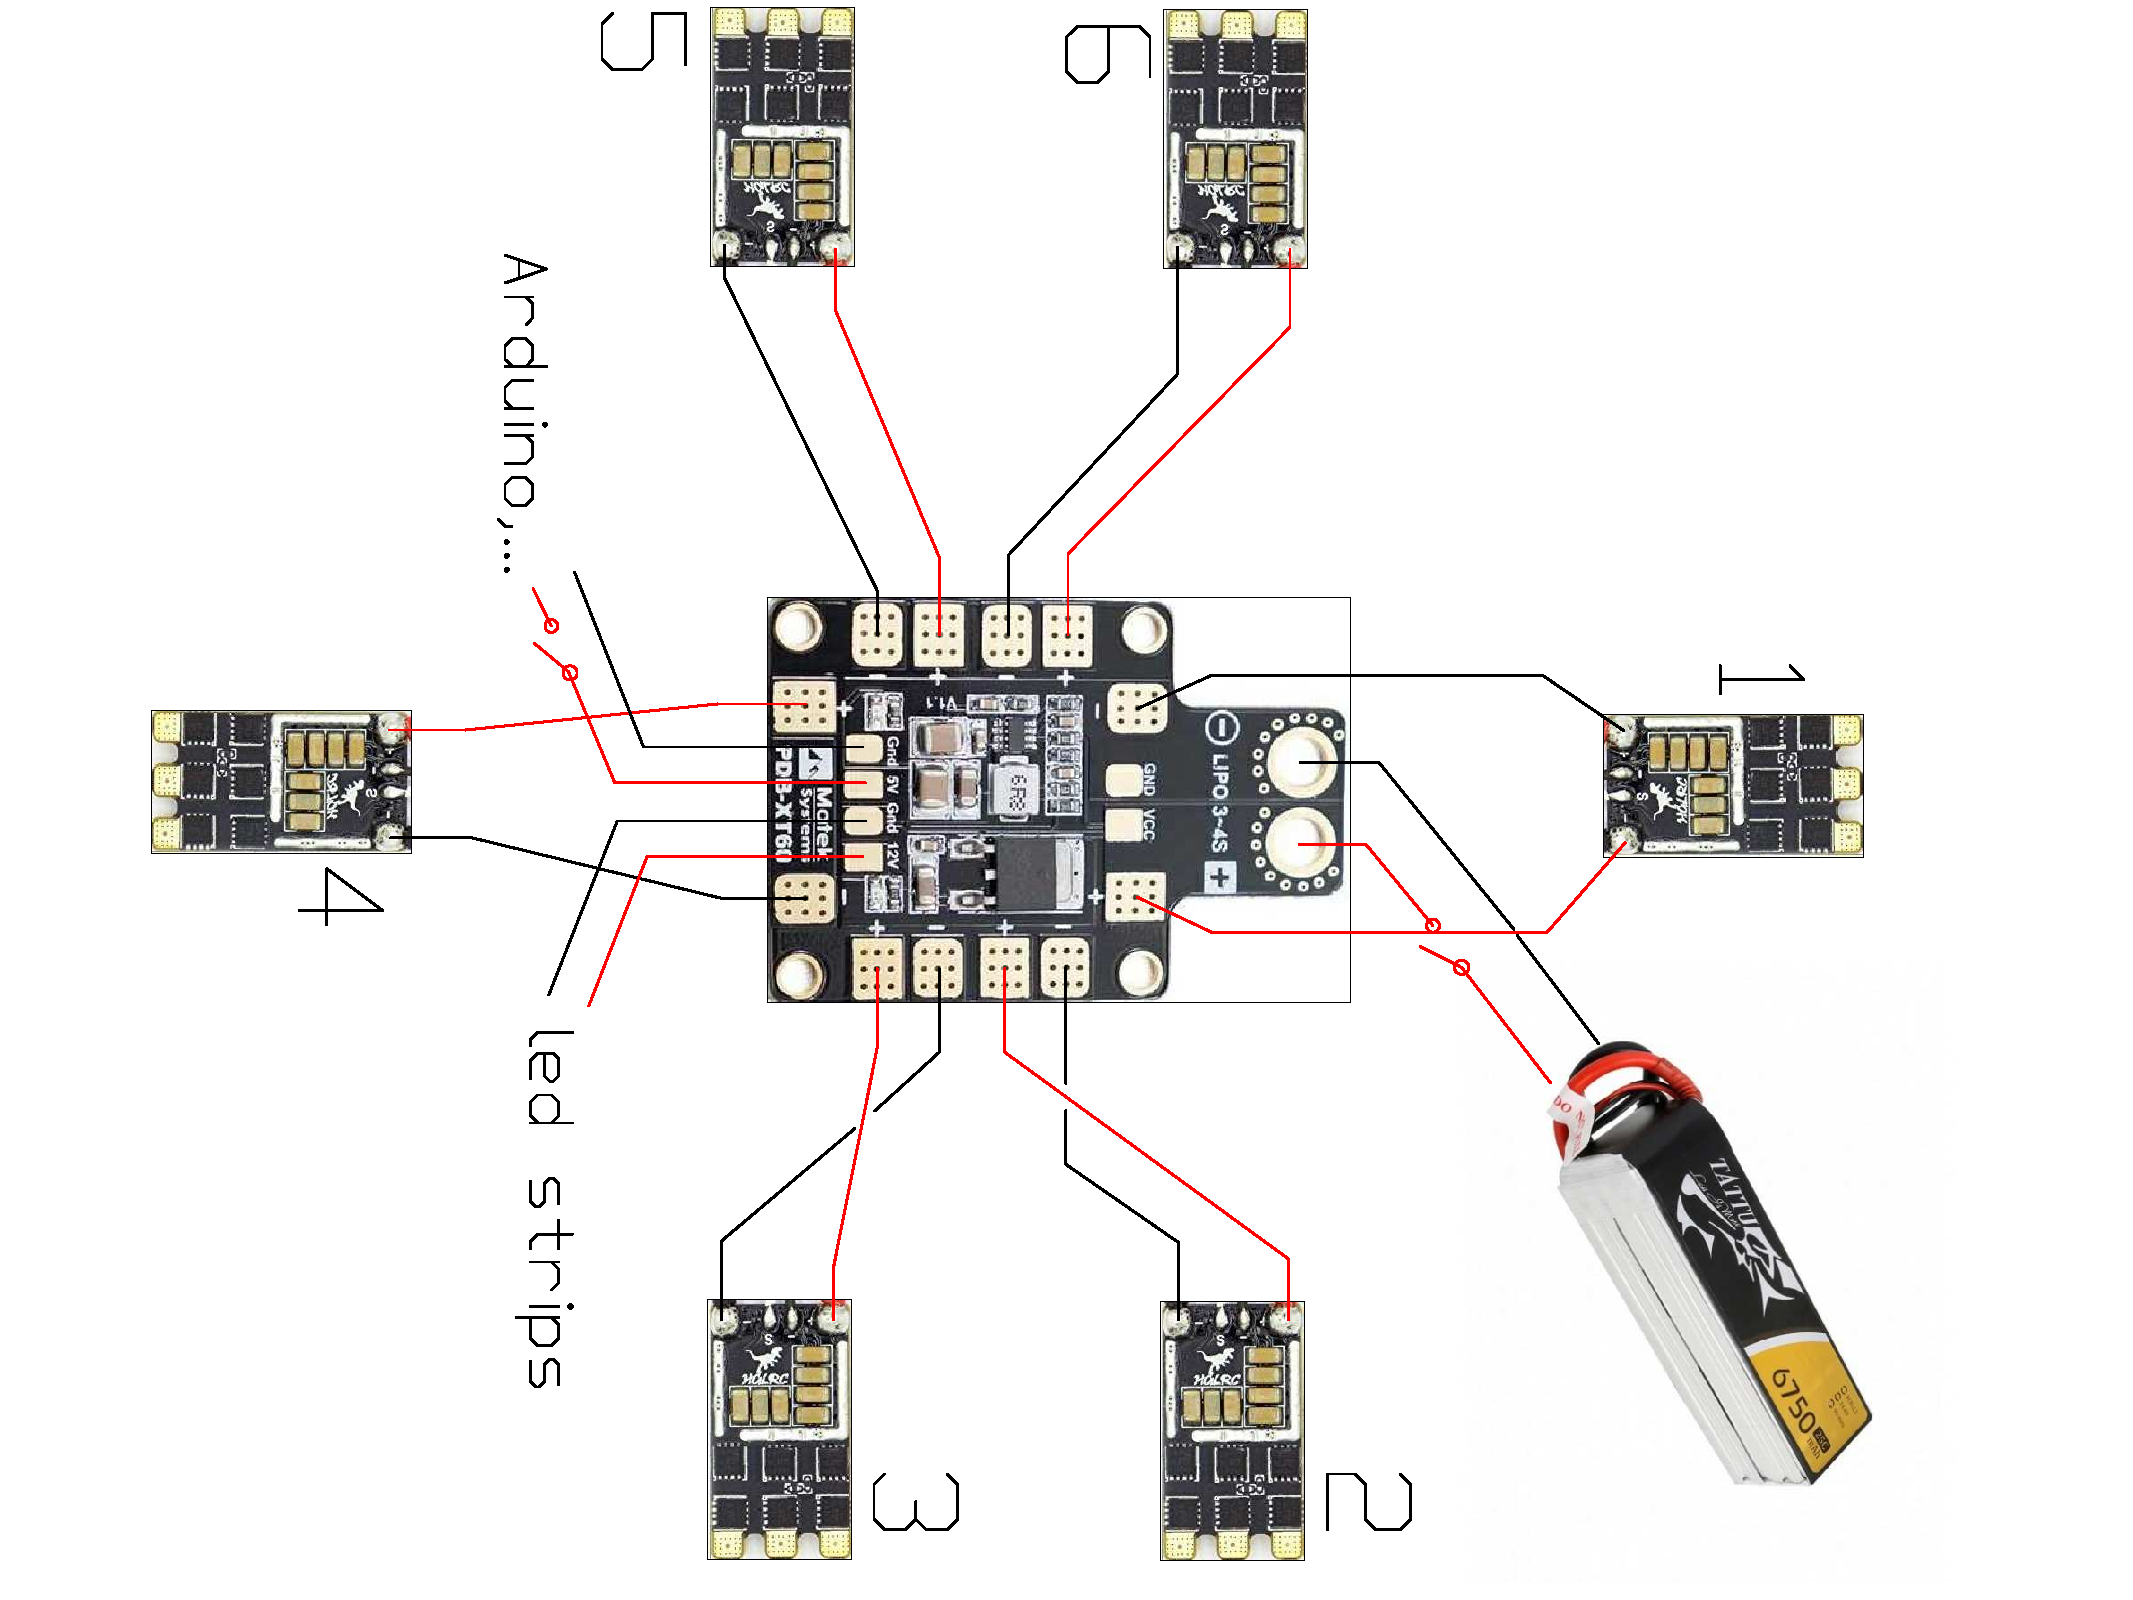
\includegraphics[width=10cm]{pictures/pdb_com.pdf}
	\caption{Schéma zapojení napájení motorů}
\end{figure}
\chapter{Testování}
\label{6-testovani}

\section{IMU filtry}
Pro použítí ovládání drona byly uvažovány dvy filtry Mahonyho a komplementární. Jednotlivé filtry byly testovány, jak obrazově tak i numericky.\\
Obrazově byla testována reakce na pohyb a ustálení polohy.
Po reakční stránce a ustálení  polohy byl lepší komplementární filtr. Vzhledem k jednoduchosti filtru, reakční doba IMU jednotky je minimální. Výsledky jsou patrné z grafů.\\
Numericky byl testován rozptyl střední hodnoty. Byla použita data po ustálení polohy v časovém intervalu čtyř minut. Výsledky byly rovnocené, oba filtry měli rozptyl střední hodnoty v řádek setin stupně.\\
Pro ovládání drona je potřebná rychlá reakce IMU, proto byl použit komplementární filtr.\\
\begin{figure}[h]
	\centering
	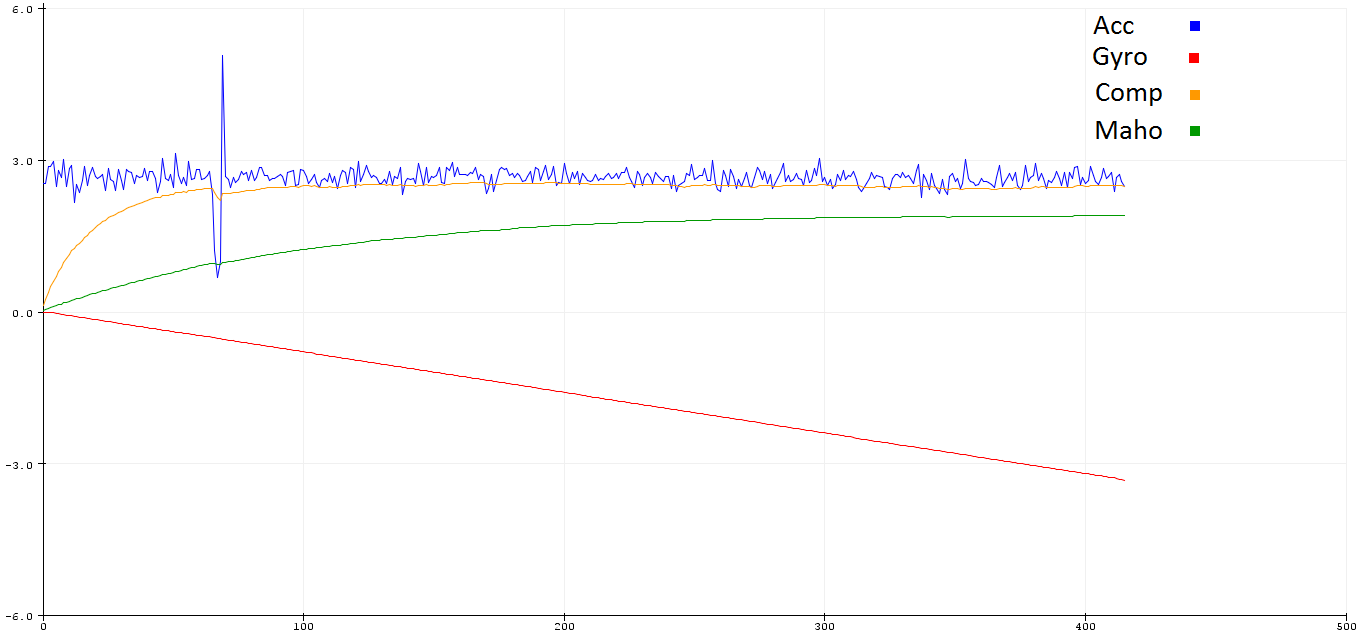
\includegraphics[width=14cm]{pictures/testRoll}
	\caption{Inicializace IMU}
\end{figure}

\begin{figure}[h]
	\centering
	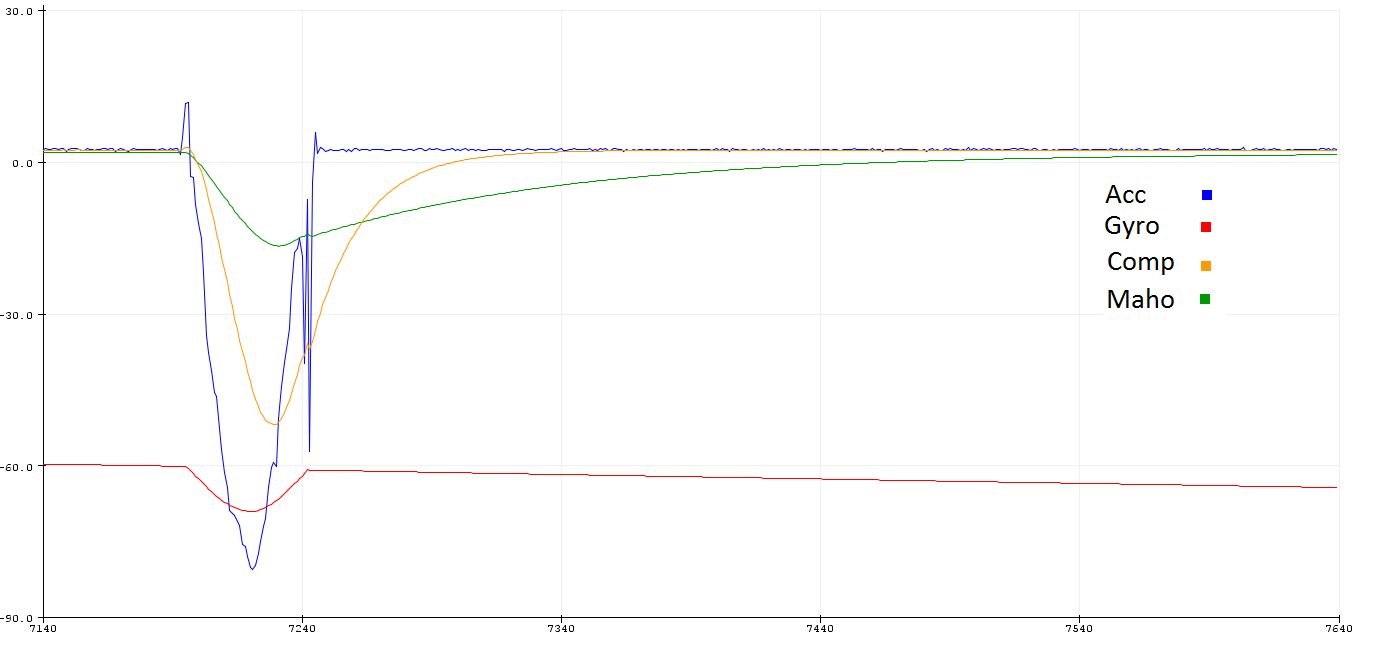
\includegraphics[width=14cm]{pictures/testRoll1}
	\caption{Náklon IMU jednotky}
\end{figure}

\section{Létající kontrolér}
Testování algoritmu létajícího kontorléru bylo prováněno na vyrobené konstrukci. Konstrukce se skládá ze čtyř latěk, které tvoří rám. Uprostřed je upevněná kovová trubka, na které se pohybuje dron. Dron je pevně připevněn k trubce tak, aby pohyboval po obvodu trubky. Na stranách trubky jsou umístěny molitanové pruhy kvůli tlumení nárazu stojánku drona. Konstukcí je docíleno simulování stavu letu s jedním stupněm volnosti. \\
Na konstrukci byla prováděna kalibrace PID regulátoru pro úhly pitch a roll. Kalibrace byla úspěšná při dostažení stabilizace drona na trubce. Kalibrace byla prováděna pro úhel pitch, výsledky kalibrace se použijí i pro úhel roll.\\
Prvně byl zjištován koeficient pro proporcionální složku. Koeficient bal navyšován do doby, než výkon vrtule dokázal drona srovnat z nakloněné polohy do vodorovné. Derivační koeficient byl zvyšován do doby, kdy PD regulátor dokázal drona stabilizovat ve vodorovné poloze. Integrační koeficient pouze doladil průběh PID regulátoru.\\


\begin{figure}[h]
	\centering
	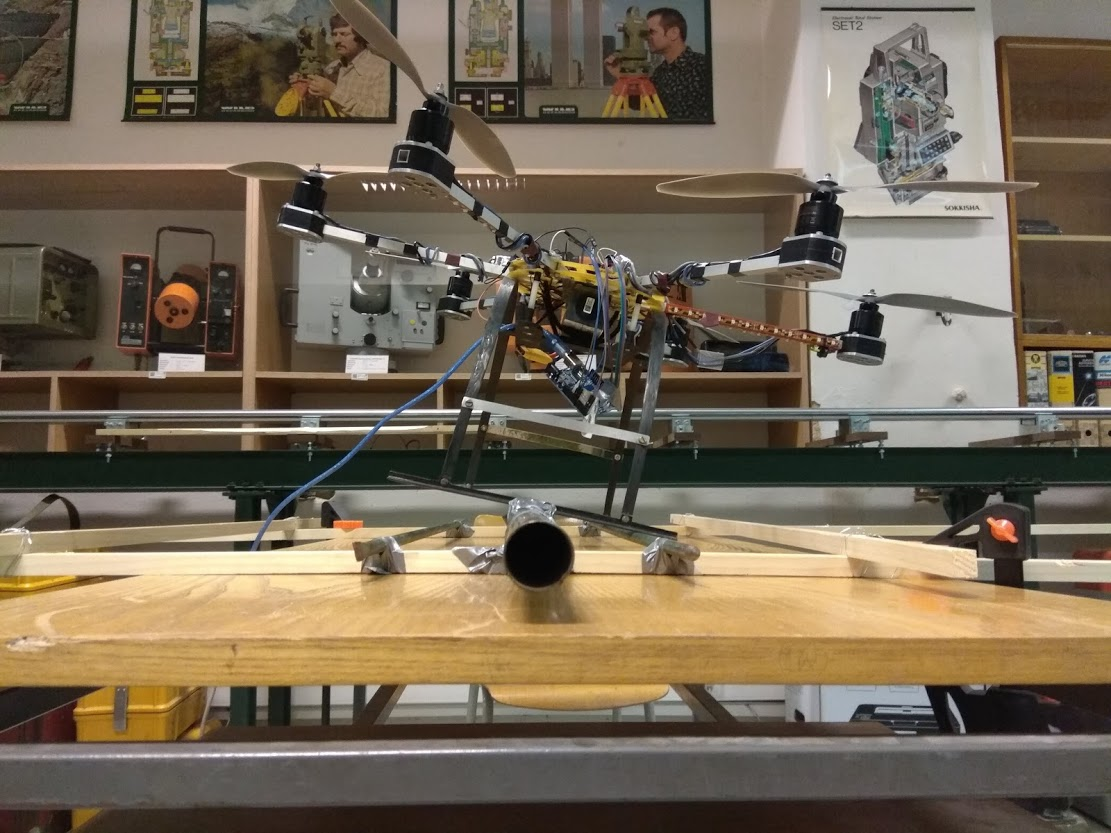
\includegraphics[width=10cm]{pictures/pidtest.jpg}
	\caption{Testování v konstrukci}
\end{figure}
\chapter{Ovládání}
\label{7-aplikace}
Pro ovládání dronu byla vytvořena aplikace pro mobilní operační systém Android. Aplikace byla napsána v programovacím jazyku Java a programovacím prostředí Android studio.\cite{android} \cite{codemitch}\\
Aplikace využívá Bluetooth a GNSS mobilu. Přes bluetooth modul probíhá přenos dat pro ovládání dronu, GNSS slouží pro zjištování polohy uživatele a zobrazení na okně s Google Maps.\\

\section{Hlavní obrazovka}
Při otevření aplikace se na display zobrazí hlavní obrazovka. Zde má uživatel na výběr zda využije manuální či autonomní ovládání. Po rozkliknutí jednoho ze spárovaných bluetooth zařízení, aplikace otevře okno pro ovládání.\\
\begin{figure}[H]
	\centering
	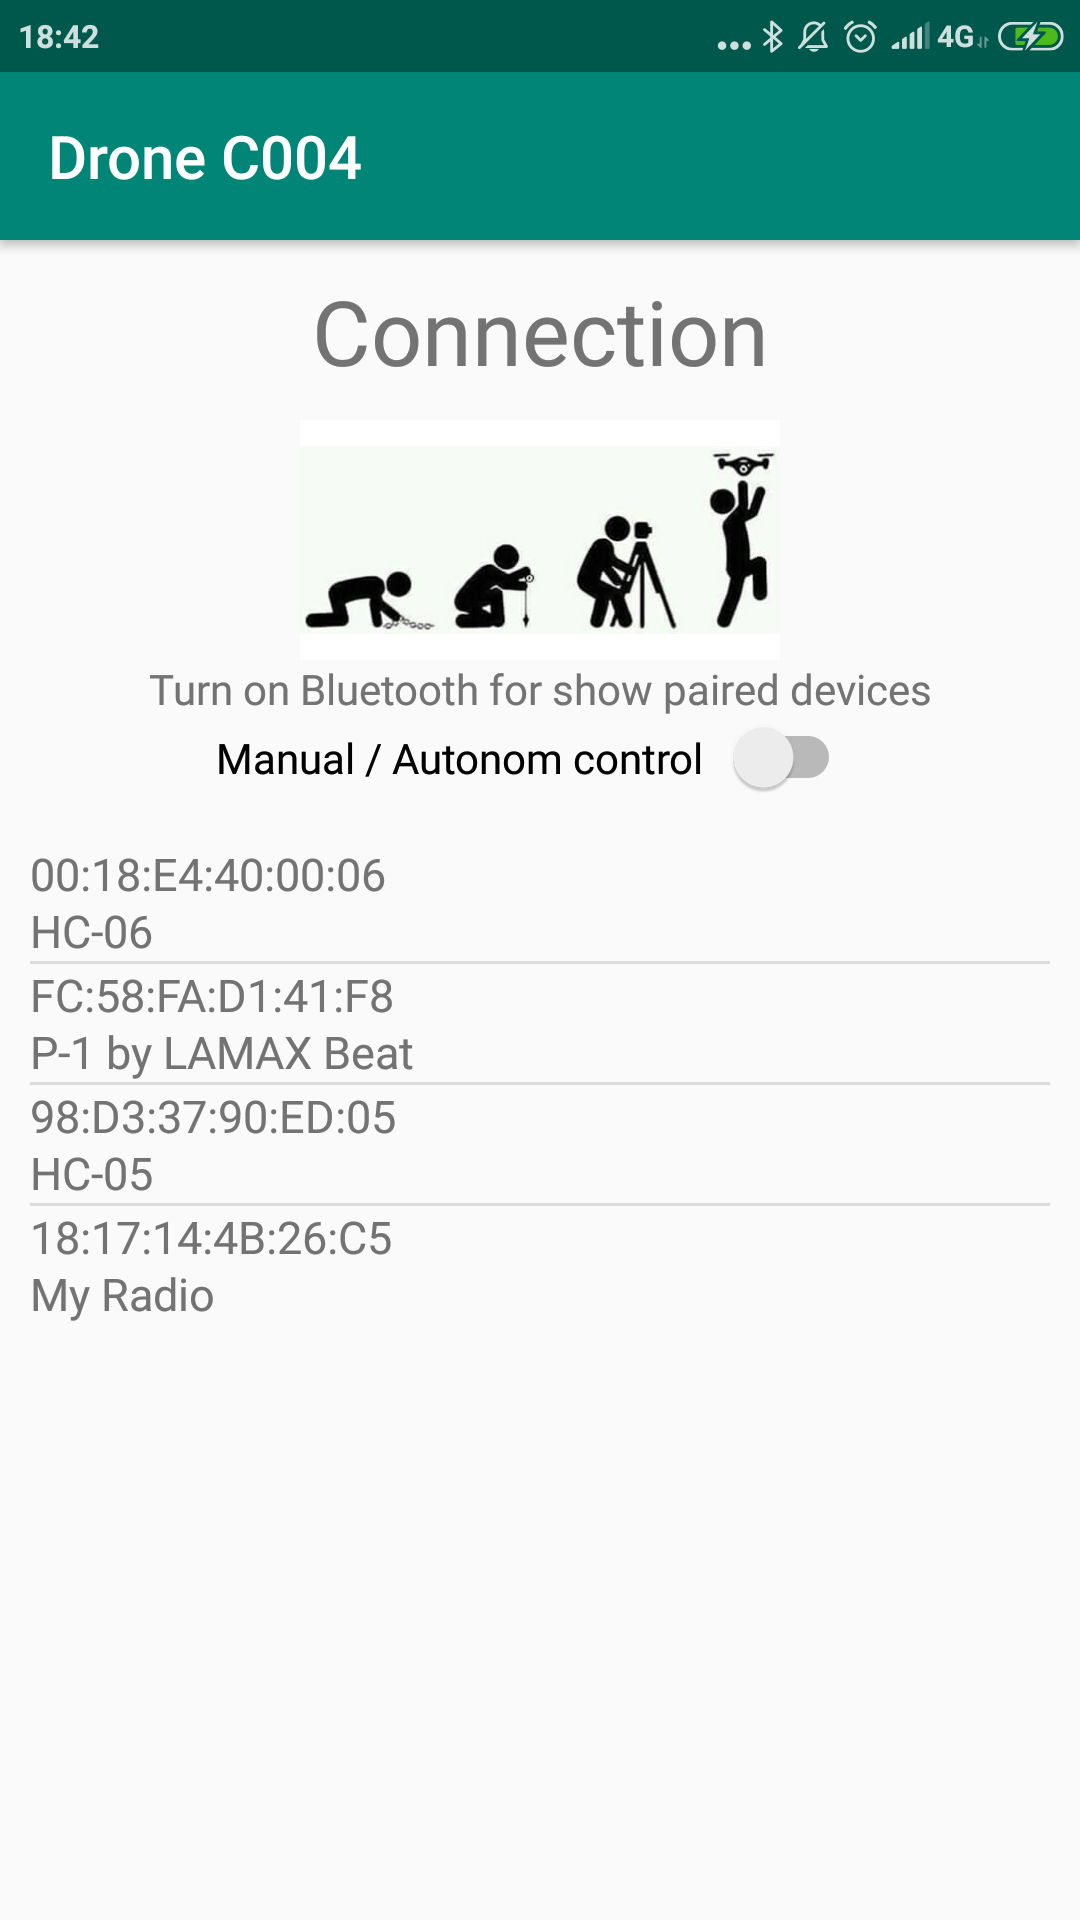
\includegraphics[width=6cm]{pictures/app1.png}
	\caption{Screenshot hlavní obrazovky}
\end{figure}

\section{Manuální ovládání} 
Manuální ovladání funguje totožně jako RC soustava. Levý joystick slouží k ovládání náklonů pitch a roll, pravý joystick slouží k ovládání throttle a yaw. Informace o poloze joystiků jsou posílány přes bluetooth komunikaci do uzlového zařízení. Typ zprávy je popsán v kapitole komunikační protokol.\\
Při tvorbě joysticků byla použita knihovna Virtuální joystick, u kterého byl upraven rozsah snímaných souřadnic ukazatele a definování jiných předávaných parametrů. Předávácí parametry byly polární souřadnice, po změně jsou předávány kartézské souřadnice joysticku. \cite{joystick}\\\\

\begin{figure}[H]
	\centering
	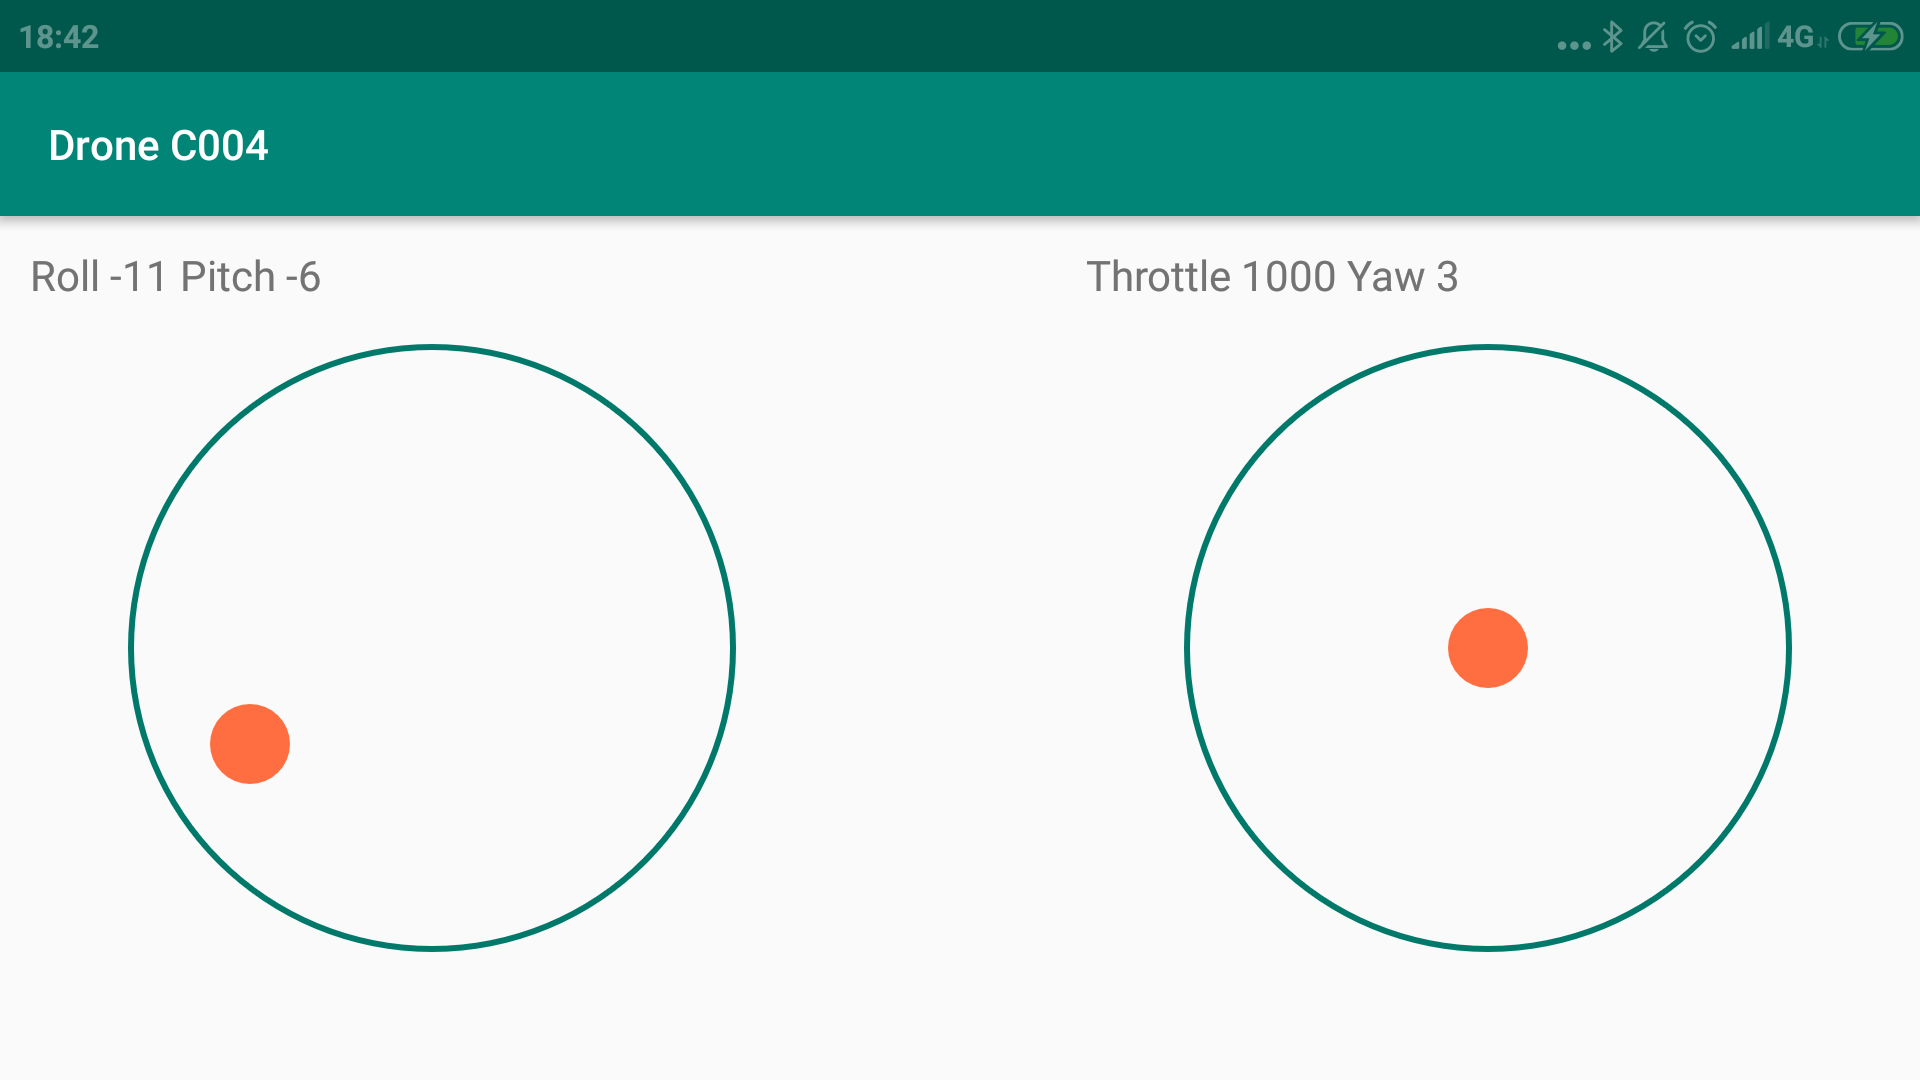
\includegraphics[width=10cm]{pictures/app.png}
	\caption{Schreenshot obrazovky pro manuální ovládání}
\end{figure}

\begin{figure}[H]
	\centering
	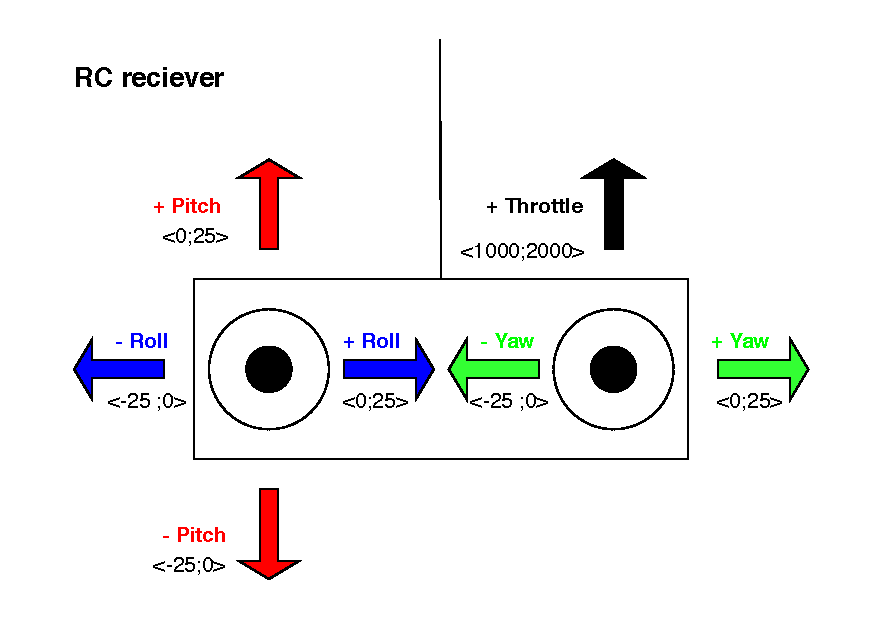
\includegraphics[width=14cm]{pictures/rcDiagram.pdf}
	\caption{Diagram RC soustavy}
\end{figure}

\section{Autonomní ovládání} 
Pro autonomní ovládání stačí zadat souřadnice v systému WGS-84. Přes tlačítko SEND je zaslat dronu a uživatel může na mapě sledovat, kde se dron nachází. Spodní tlačítko Home slouží k návratu dronu a startovní místo. Autonomní ovládání je též ve vývoji, zprovoznění bude možné až po dokončení navigačního kontroléru.\\
Mapa je generována ze serverů Google Maps přes API. API je možné používat po registraci pro google vývojáře a nastavení API pro aplikaci.\\

\begin{figure}[H]
	\centering
	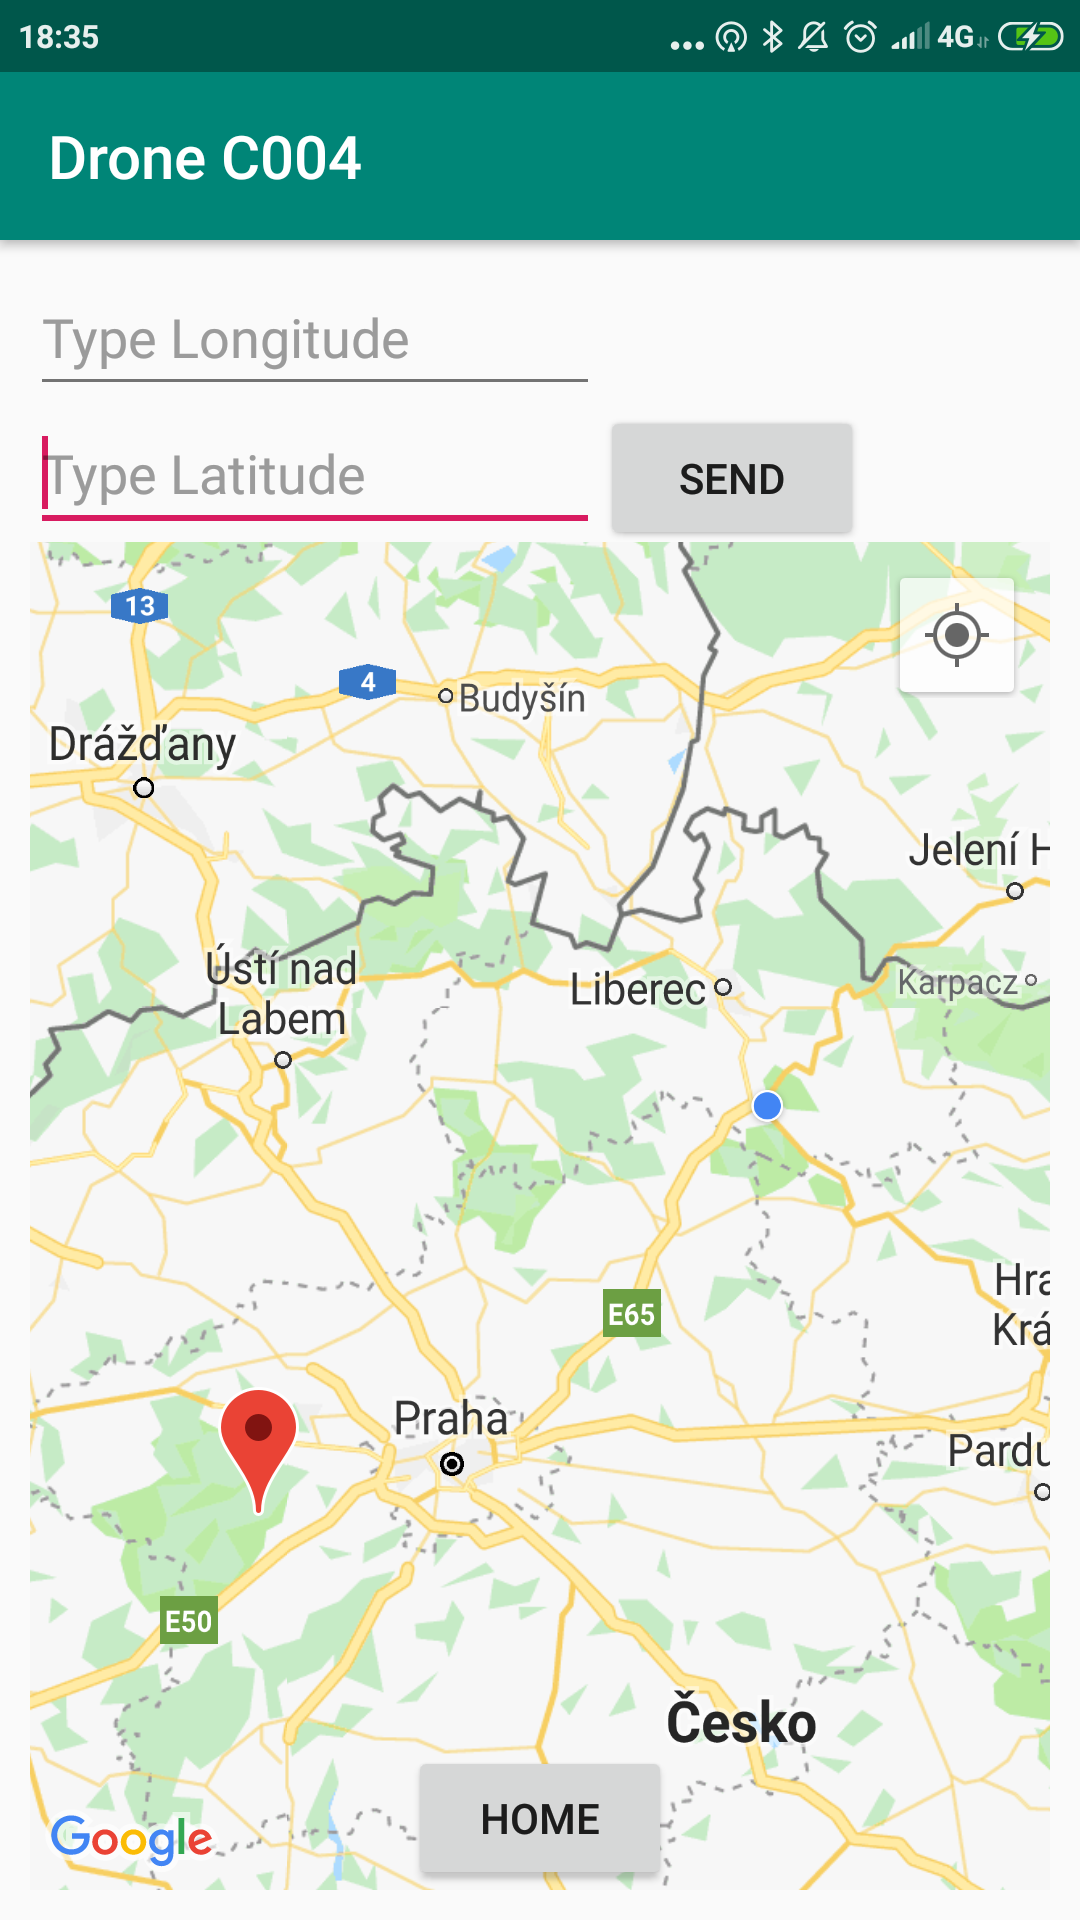
\includegraphics[width=6cm]{pictures/app2.png}
	\caption{Schreenshot obrazovky pro autonomní ovládání}
\end{figure}

\section{Kamera}
Bylo v plánu implementovat obraz z kamery z dronu do mobilní aplikace. Bohužel pro nedostatek času a málo zkušeností s Android studiem je tato část pouze rozpracovaná. Pro zobrazení obrazu v aplikaci byla použita více platformová knihovna libusb a libuvc.\\
Obraz z kamery lze sledovat přes mobilní aplikaci FPViewer. Po zapojení přijímače obrazového signálu se aplikace automaticky zapne.\\

\begin{figure}[H]
	\centering
	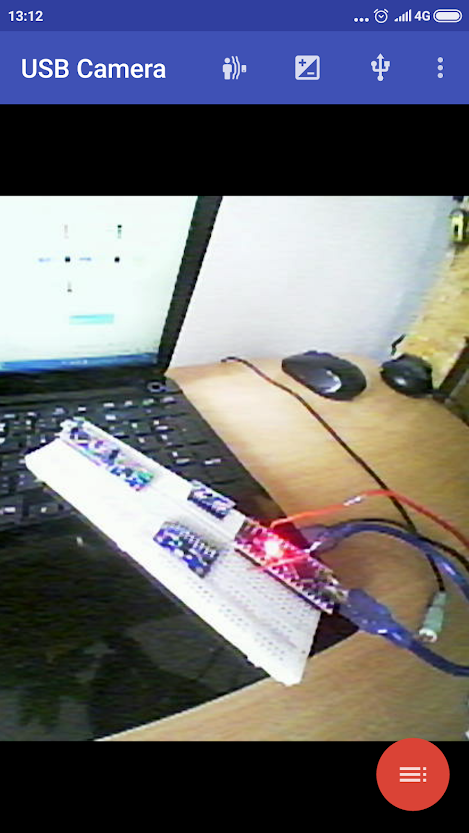
\includegraphics[width=6cm]{pictures/fpvscreenshot.png}
	\caption{Schreenshot aplikace FPViewer}
\end{figure}


\chapter{Závěr}
\label{8-zaver}
Stavba dronu není lehký úkol, zvlášť pro někoho, kdo neumí elektrotechniku, ale pokud existuje nápad, jak dál rozvíjet geodezii, je potřeba se ho chytit. Postupným studováním problematiky dronů se zvětšovalo množství potřebných informací. Jednoduše, čím více jsem informací věděl, tím více jsem zjišťoval, že vlastně nic nevím.\\
Prvně se práce měla věnovat nadstavbovým geodetickým úlohám nad dronem od firmy Microkopter. U zapůjčeného dronu pouze nefungovala radiová komunikace. Chtěl jsem vyměnit komunikační zařízení a s dronem začít létat, bohužel ovládací prvky se nedaly přeprogramovat a ani nefungovala komunikace prvků s počítačem. Z dronu se odebraly kontroléry a zůstala kostra s motory a regulátory otáček. Po pár testování jeden z regulátorů zkratoval a jelikož byl regulátor od firmy Microkopter drahý, byl nahrazen jiným (uvedený v komponentách).\\
Tím začala stavba dronu od nuly. Nové regulátory měly odlišný způsob komunikace a jiný způsob zapojení. Bohužel i zapůjčené baterie byly poškozené, z důvodu dlouhodobého nepoužívání.\\
Pro komunikaci kontroléru s regulátory byla prvně použita knihovna Servo. Spousta článků a projektů používaly Servo knihovnu pro komunikaci s regulátory. Po pár neúspěšných testech letového kontroléru, jsem zjistil, kde spočívá problém. Knihovna servo dokáže komunikovat s regulátory, ale pouze s frekvencí 50Hz. Pro let dronu musí být frekvence výpočtu a ovládání regulátorů větší než 100Hz. Proto jsem musel implementovat standartní PWM komunikační protokol pro regulátory. Komunikační protokol je závislý na době trvání výpočtu. S použitím platformy Arduino byla docílená frekvence ovládání regulátorů 250Hz.\\
S IMU jednotkou byly tež problémi. Při použití knihovny pro modul MPU9250, bylo čtení dat z modulu pomalé. Proto byl nastudován popis modulu a modul byl ovládán přes komunikaci I2C za použití registrů.\\
Pro ovládání byla vytvořena aplikace pro operační systém Android a v programovacím jazyku Java. Jedná se o první aplikaci, kterou jsem kdy dělal. Na internetu je spousta návodů podle, kterých se dá naučit programovat aplikaci, i dokumentace Android Developers mi hodně pomohla. Bohužel se nepodařilo do aplikace implementovat obraz z kamery. Pro zprovoznění kamery bylo potřeba importovat knihovny v jiných programovacích jazycích, nastavit jejich sestavení. Nynější stav je, že kamera je připojená k aplikaci, ale nic nezobrazuje.\\
Jak bylo zmíněno na začátku, stavba dronu není lehký úkol. Proto práce se zabývá pouze stavbou a už ne geodetickými nadstavbami. S konstrukcí dronu bych chtěl pokračovat a zrealizovat nápady uvedené v úvodu.\\

\include{9-dokumentace}

% Vysázení seznamu zkratek

\begin{seznamzkratek}{ABCDE}  
	
      \novazkratka{CCW}
			{CCW}
			{údaj o směru otáčení proti směru hodinových ručiček  (counter clockwise)}
	
	 \novazkratka{CW}	
			{CW}
			{údaj o směru otáčení po směru hodinových ručiček (clockwise)}    
	      
	 \novazkratka{I2C}
	      {I2C}
	      {počítačová sériová sběrnice (Inter-Integrated Circuit)}
	      
	\novazkratka{LiPo}
		  {LiPo}
	      {Lithium-polymerový akumulátor}
	      
	      
	\novazkratka{SCL}
	      {SCL}
	      {vodič pro přenos hodinové signálu (Serial Clock)}
	      
	\novazkratka{SDA}
	      {SDA}
	      {vodič pro přenos datového signálu (Serial Data)}
	      
	\novazkratka{SPI}
	      {SPI}
	      {sériové periferní rozhraní (Serial Peripheral Interface)}
	      
	\novazkratka{SCLK}
		  {SCLK}
		  {vodič pro přenos hodinové signálu (Serial Clock)}
		  
	\novazkratka{MOSI}
		  {MOSI}
		  {vodič pro jednosměrnou komunikaci hlavního do vedlejšího zařízení (Master Out, Slave In)}
		  
	\novazkratka{MISO}
		  {MISO}
		  {vodič pro jednosměrnou komunikaci vedlejšího do hlavního zařízení (Master In, Slave Out)}
		  
	\novazkratka{SS}
		  {SS}
		  {vodič pro určení vedlejšího zařízení (Slave Select)}
      
	\novazkratka{PDB}
	      {PDB}
	      {distribuční deska  (Power Distribution Board)}

	  \novazkratka{BLDC}	
	      {BLDC}
	      {Bezkartáčové stejnosměrné motory (brush less direct curent)}
	      
	  \novazkratka{ESC}	
	      {ESC}
	      {Regulátor otáček (Electronic speed control)}	      
	    
	   \novazkratka{VCC}	
	      {VCC}
	      {Napětí na společném kolektoru (Voltage at the Common Collector)} 
  
  	   \novazkratka{GND}	
  		  {GND}
          {Zem (Ground)} 
          
       \novazkratka{S}	
          {S}
          {Ovládací pin (Signal pin)} 

       \novazkratka{IMU}	
		  {IMU}
          {Inerciální měřící jednotka (Inertial Measurement Unit)} 
          
       \novazkratka{GNSS}	
          {GNSS}
          {Globální družicový polohový systém (Global Navigation Satellite System)} 
          
       \novazkratka{PWM}	
          {PWM}
          {Pulzně šířková modulace (Pulse Width Modulation)}
          
       \novazkratka{PPM}	
          {PPM}
          {Pulzně polohová modulace (Pulse position Modulation)}
          
          
       \novazkratka{RTK}	
          {RTK}
          {Metoda GNSS (Real Time Kinematic)}
          
       \novazkratka{USB}	
          {USB}
          {Univerzální seriový konektor (Universal Serial Bus)}
          
       \novazkratka{FPV}	
          {FPV}
          {Pohled z první osoby (First person view)}
          
       \novazkratka{PRPM}	
          {RPM}
          {otáčky za minutu (revolutions per minute)}
          
       \novazkratka{bps}	
          {bps}
          {bity za sekundu (bit per second)}
          
       \novazkratka{OTG}	
          {OTG}
          {funkce USB (On The Go)}
          
        \novazkratka{API}	
          {API}
          {Rozhraní pro programování aplikací (Application Programming Interface)}

\end{seznamzkratek}


% Literatura
\nocite{*}
\def\refname{Literatura}
\bibliographystyle{mystyle}
\bibliography{literatura}


% Začátek příloh
\def\figurename{Figure}%
\prilohy

% Vysázení seznamu příloh
%\seznampriloh

% Vložení souboru s přílohami
%%%%%%%%%%%%%%%%%%%%%%%%%%%%%%%%%%%%%%%%%%%%%%%%%%%%%%%%%%%%%%%%%%%%%%%%%%%%%%%%%%%
%%                 PŘÍLOHA - UŽIVATELSKÁ PŘÍRUČKA                                %%
%%%%%%%%%%%%%%%%%%%%%%%%%%%%%%%%%%%%%%%%%%%%%%%%%%%%%%%%%%%%%%%%%%%%%%%%%%%%%%%%%%%
\chapter{Dokumentace}
\label{user-guide}


\section{Flying Control}
\label{installation-manual}


\section{Obstacle Control}

\section{Navi Control}

% Konec dokumentu
\end{document}
